\documentclass[10pt,UKenglish, leqno, xcolor = dvipsnames]{beamer}

\usetheme{UiB}

% Font choice:
\usefonttheme{default}

\usepackage{cite}
\usepackage{amsmath, amsthm, mathtools, color, setspace}
\usepackage{fancyhdr, braket, etoolbox,booktabs,multirow}
\usepackage{xfrac, lmodern, ifsym, bm, multicol, booktabs, pdflscape}
\usepackage[utf8]{inputenx} % For æ, ø, å
\usepackage{csquotes}       % Quotation marks
\usepackage{microtype}      % Improved typography
\usepackage{amssymb}        % Mathematical symbols
\usepackage{mathtools,physics,centernot,tensor}      % Mathematical symbols
\usepackage[absolute, overlay]{textpos} % Arbitrary placement
\setlength{\TPHorizModule}{\paperwidth} % Textpos units
\setlength{\TPVertModule}{\paperheight} % Textpos units
\usepackage[dvipsnames]{xcolor}
\usepackage{tikz}
\usetikzlibrary{tikzmark,calc,overlay-beamer-styles,arrows,shapes}  % Overlay effects for TikZ
\newenvironment{proenv}{\only{\setbeamercolor{local structure}{fg=RoyalBlue}}}{}
\newenvironment{conenv}{\only{\setbeamercolor{local structure}{fg=Maroon}}}{}
\newenvironment{bibbianoenv}{\only{\setbeamercolor{local structure}{fg=Green}}}{}
\DeclarePairedDelimiter{\insieme}{\{}{\}}
\newcommand{\numberset}{\mathbb}
\newcommand{\alg}{\mathfrak}
\newcommand{\Z}{\numberset{Z}}
\newcommand{\R}{\numberset{R}}
\newcommand{\N}{\numberset{N}}
\newcommand{\C}{\numberset{C}}
\newcommand{\A}{\alpha}




\author{Pietro Daniele}
\title{\large Search for resonances in the 105 to 200 GeV diphoton invariant mass range using 140 fb$^{-1}$ of pp collisions collected at $\sqrt{s}$=13 TeV with the ATLAS detector}

\begin{document}
	\tikzstyle{na} = [baseline=-.5ex]
	\tikzstyle{every picture}+=[remember picture]
	
	\begin{frame}{Project description}
		\vfill
		A search for new spin-0 resonances:
		\begin{itemize}
			\item a blind search in [110,170] GeV $m_{X}$ range;
			\item fitting in [105,200] GeV $m_{\gamma\gamma}$ range;
			\item Use SM Higgs boson samples at different masses to model the signal;
			\item a production mode independent model:
			\begin{itemize}
				\item only \textit{ggF} production mode is considered, the others are used to create a systematic uncertainty of efficiency;
				\item the signal model is a function of $m_H$;
			\end{itemize} 
			\item the events selected are pairs of high-pt and isolated photons; 
			\item the events are classified into mutually exclusive categories;
			\item the signal is modeled fitting simulated \textit{ggF} MC samples in each category;
			\item the background is fitted from data.
		\end{itemize}
		\vfill
	\end{frame}
	
	\begin{frame}{MC samples}
		\vfill
		\textit{h026} MC samples are obtained by merging and weighting the three flavours (mc16a, mc16d, mc16e):
		\begin{itemize}
			\item Signal $\to$ \textit{ggF} MC samples using different $m_H$ resonance masses (110, 125, 130, 140 GeV);
			\item Background $\to$ 3 slices \textit{Sherpa2\_diphoton}  [50,90], [90,175], [175,2000] GeV.
			\item Other production modes $\to$ \textit{VBFH, ttH, WmH, WpH, ZH} MC samples using different $m_H$ resonance masses (110, 125, 130, 140 GeV);
		\end{itemize}
		\vfill
	\end{frame}
	

	

	
	\begin{frame}{Events selection}
		\vfill
		Events selected:
		\begin{itemize}
			\item $|\eta_{S2}|$ < 2.37 excluding the crack region 1.37 < $|\eta_{S2}|$ < 1.52.
			\item at least two \textit{FixedCutLoose} isolated $\gamma$ with \textit{Tight} identification;
			\item leading photon $\rightarrow$ $p_T/m_{\gamma\gamma} > 0.35$;
			\item sub-leading photon $\rightarrow$ $p_T/m_{\gamma\gamma} > 0.25$;
		\end{itemize}
		
		\vspace{0.5cm}
		%$\Longrightarrow$ The events the \texttt{cutFlow} greater than 13 are selected.
		\vfill
	\end{frame}

	\begin{frame}{Fiducial events}
		\vfill
		Fiducial events are used in the signal model $\to$ yield, xs, systs and limits
		\begin{itemize}
			\item events $\to$ \texttt{isFiducialLowMyy = true}:
			\begin{itemize}
				\item $|\eta|<2.43$;
				\item $p_T^{\gamma_1}$ > 22 GeV;
				\item $p_T^{\gamma_2}$ > 22 GeV;
				\item $E_{T}^{cone20\ \gamma_*}/(p_T^{\gamma_*})$ < 0.065;
			\end{itemize} 
			\item eff(m$_H$) = $C_X\cdot A_X$
			\item $\sigma$ $\to$ $\sigma^{fid} = \sigma\cdot A_X$
		\end{itemize}
		\vfill
	\end{frame}
	
	\begin{frame}{Categories}
		\vfill
		The chosen categorisation (\texttt{catConvEta}) is the simplest one and it is based on the photon conversion and $|\eta_{S2}|$.\\
		$\Rightarrow$ Mass categories without the $p^{\gamma\gamma}$ selections
		
		\begin{itemize}
			\item \textbf{2 phs unconv}:
			\begin{itemize}
				\item 2 $\gamma$s with $|\eta_{s2}| < 0.75$ $\rightarrow$ \textcolor{red}{1};
				\item 2 $\gamma$s with $|\eta_{s2}|$ no central and no trans regions $\rightarrow$ \textcolor{red}{2};
				\item at least one $|\eta_{s2}|\ \epsilon\ [1.3,1.75]$ $\rightarrow$ \textcolor{red}{3};
			\end{itemize}
			\item \textbf{at least 1 ph conv}:
			\begin{itemize}
				\item 2 $\gamma$s with $|\eta_{s2}| < 0.75$ $\rightarrow$ \textcolor{red}{4};
				\item 2 $\gamma$s with $|\eta_{s2}|$ no central and no trans regions $\rightarrow$ \textcolor{red}{5};
				\item at least one $|\eta_{s2}|\ \epsilon\ [1.3,1.75]$ $\rightarrow$ \textcolor{red}{6};
			\end{itemize}
			
			\begin{textblock}{1}(0.175,0.725)
				\centering
				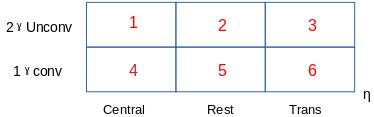
\includegraphics[width=.5\textwidth]{Pres_Images/HGam/cat_tab.png}
			\end{textblock}
		\end{itemize}
		\begin{textblock}{1}(0.42,0.84)
			\small
			$\geq$
		\end{textblock}
		\vfill
		
	\end{frame}
	
	
	
	\begin{frame}{Signal model}
		\vfill
		\begin{itemize}
			\item The signal in each category is modeled using simulated MC $H^{SM}_{spin0}\to\gamma\gamma$ as a function of the mass of the resonance;
			\item a simultaneous fit is performed on all \textit{ggF} MC samples with different $m_H$ mass, with DSCB parameters as functions of $m_H$.
		\end{itemize}
		\centering
		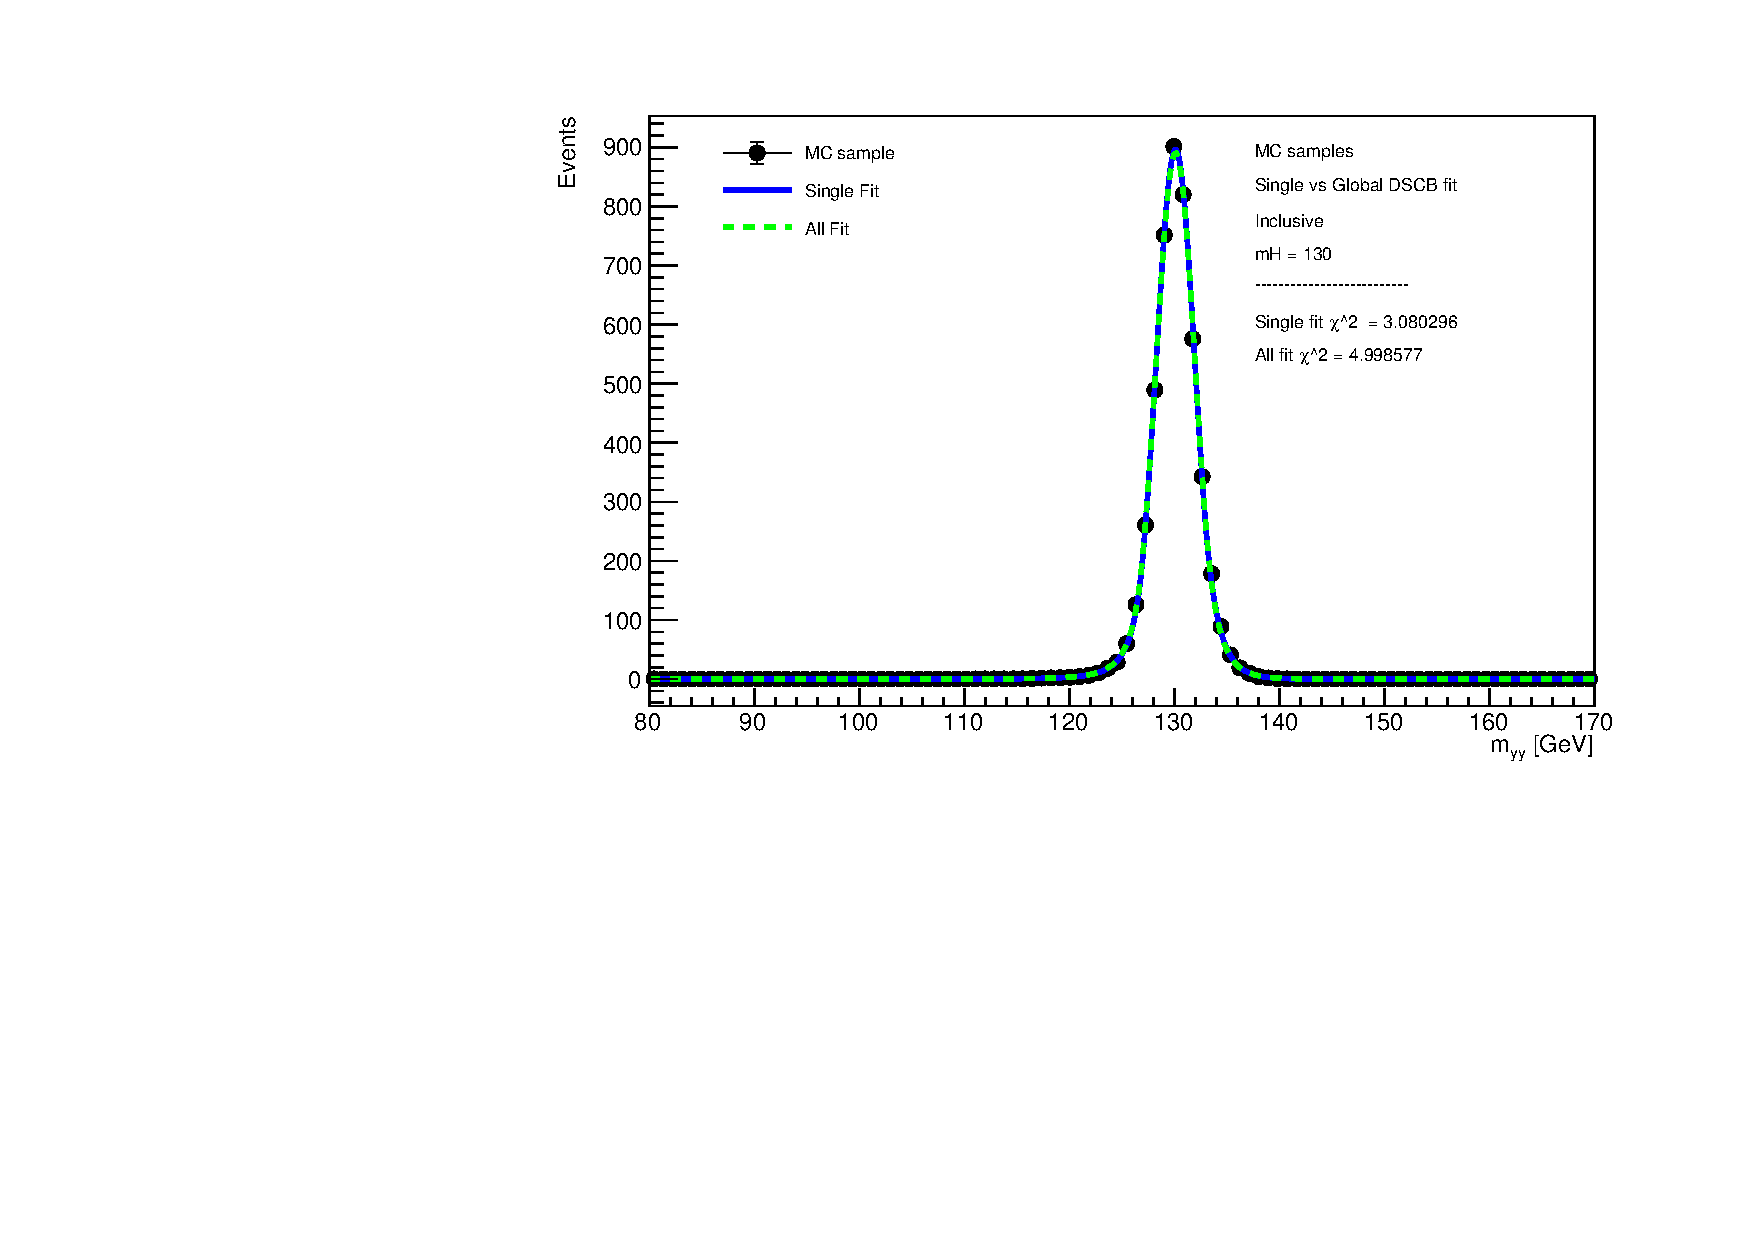
\includegraphics[width=.4\textwidth]{Pres_Images/HGam/comp_plot_130GeV.pdf}
		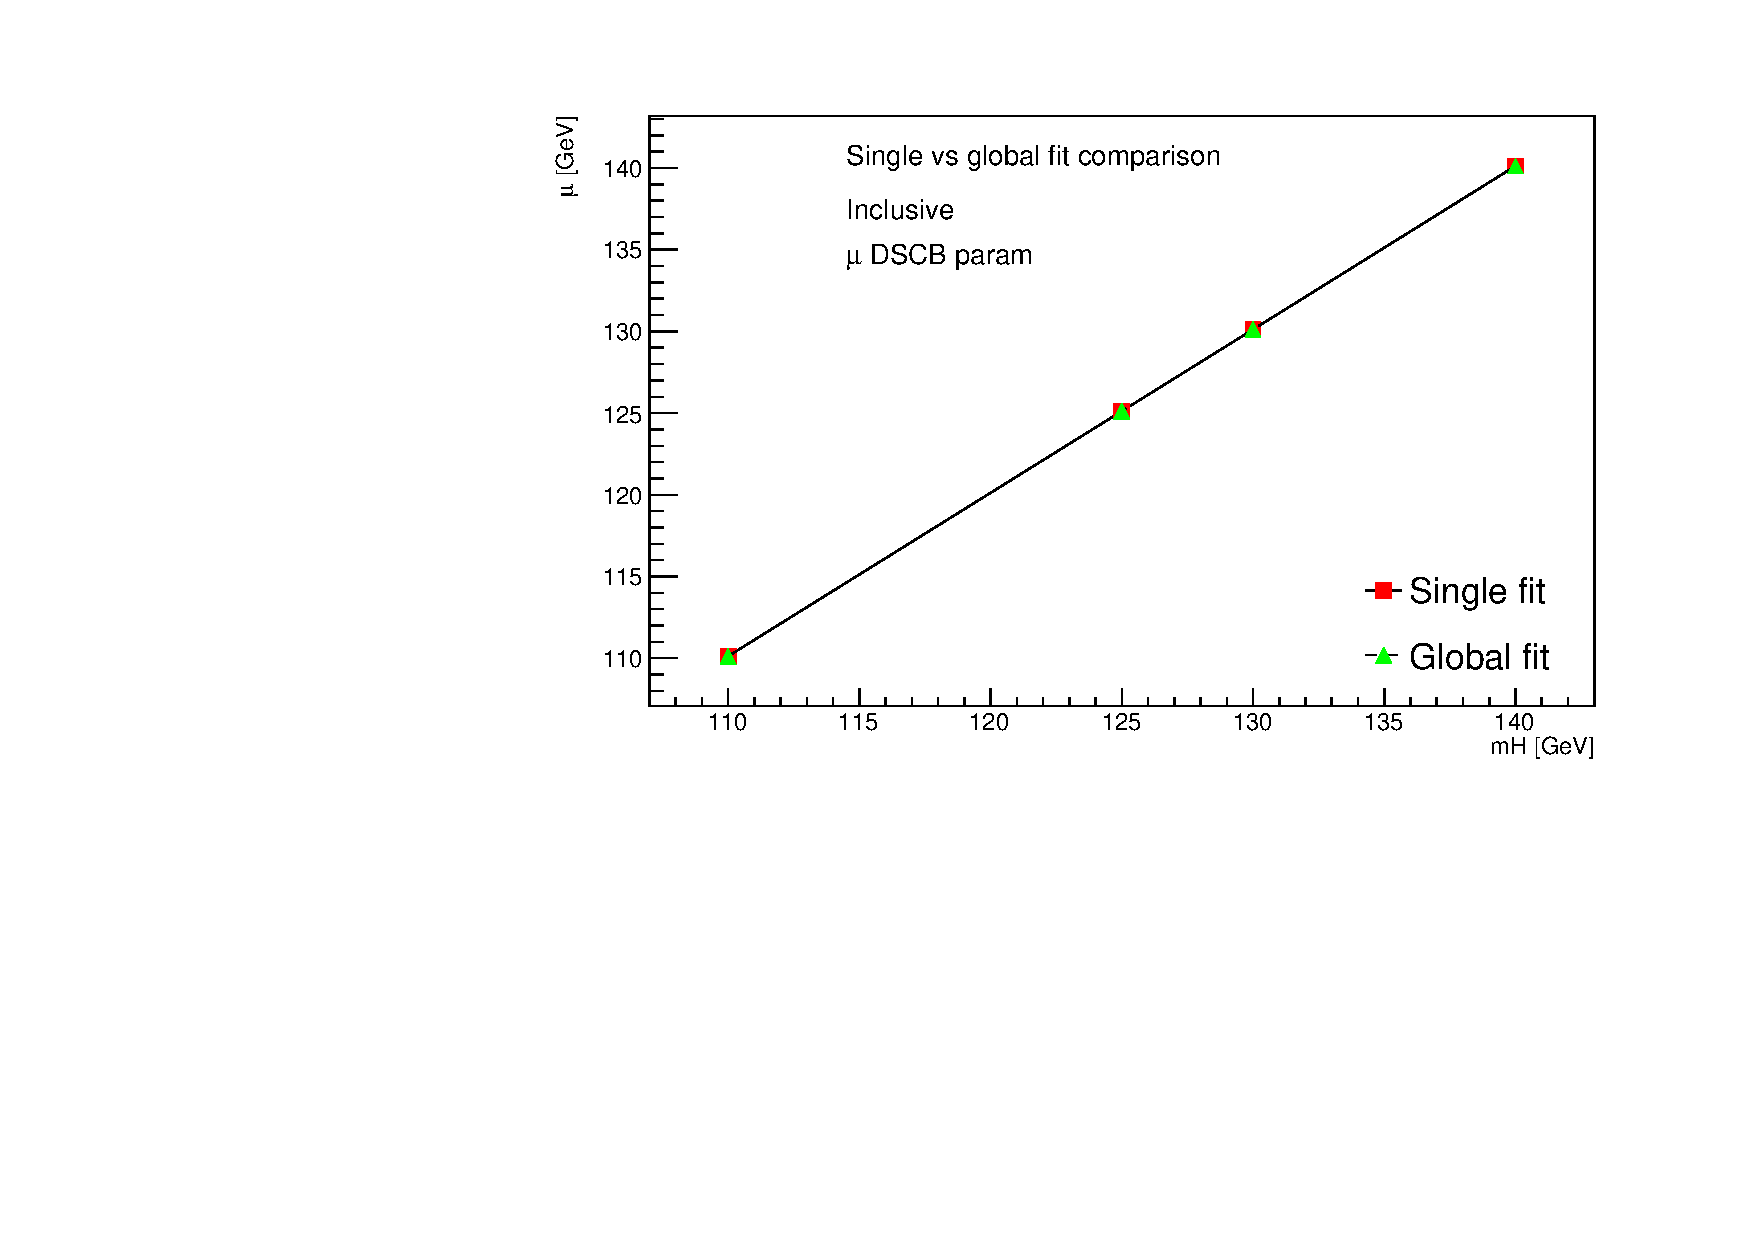
\includegraphics[width=.4\textwidth]{Pres_Images/HGam/mu_comp.pdf}\\
		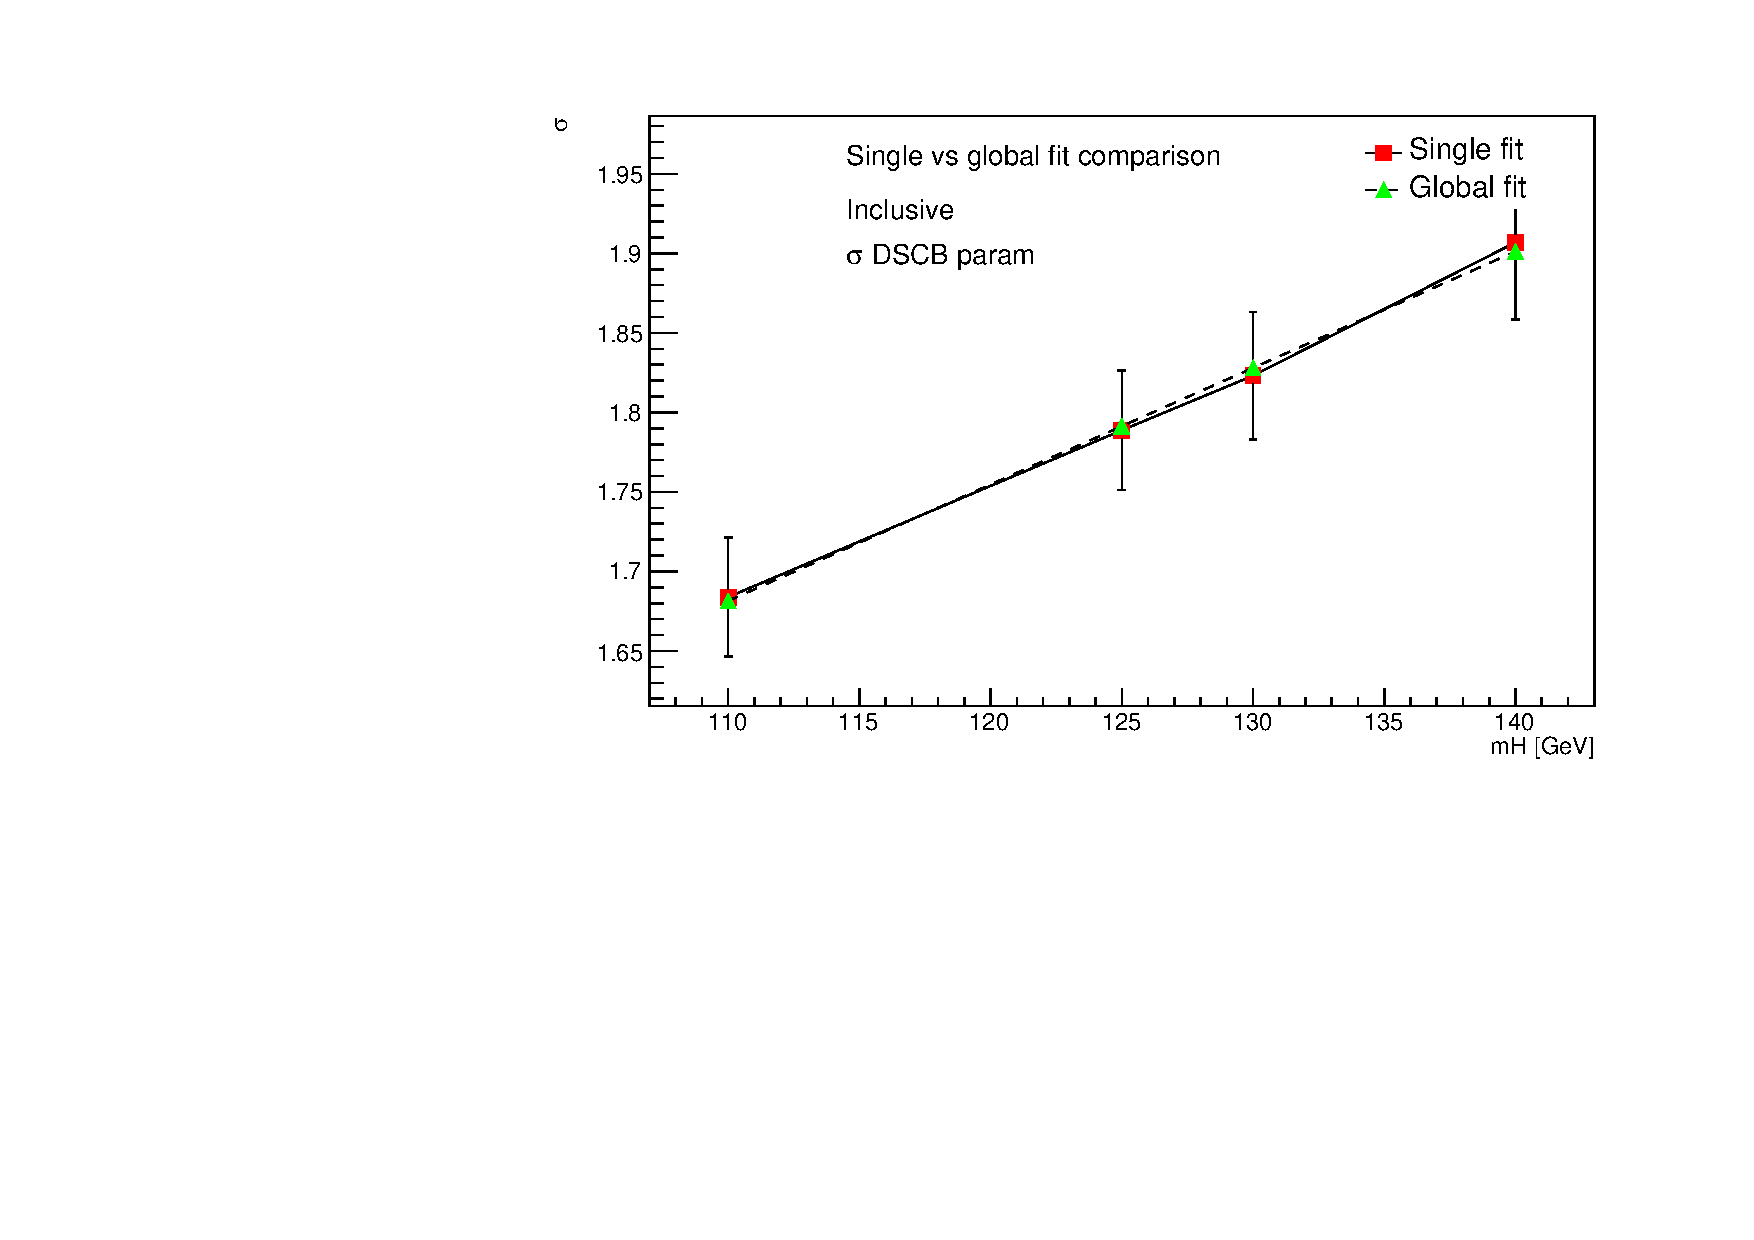
\includegraphics[width=.4\textwidth]{Pres_Images/HGam/sigma_comp.pdf}\\
		\vfill
	\end{frame}
	
	\begin{frame}{Test signal model}
		\vfill
		The signal model as a function of resonant mass is tested:
		\begin{itemize}
			\item the simultaneous fit is performed on only \textit{ggF} 110, 130 and 140 GeV MC samples;
			\item then the model is applied to the MC 125 GeV sample;
		\end{itemize}
		
		\vspace{.5cm}
		\begin{center}
			$\Rightarrow$ the model is able to fit correctly the MC 125 GeV sample
			
			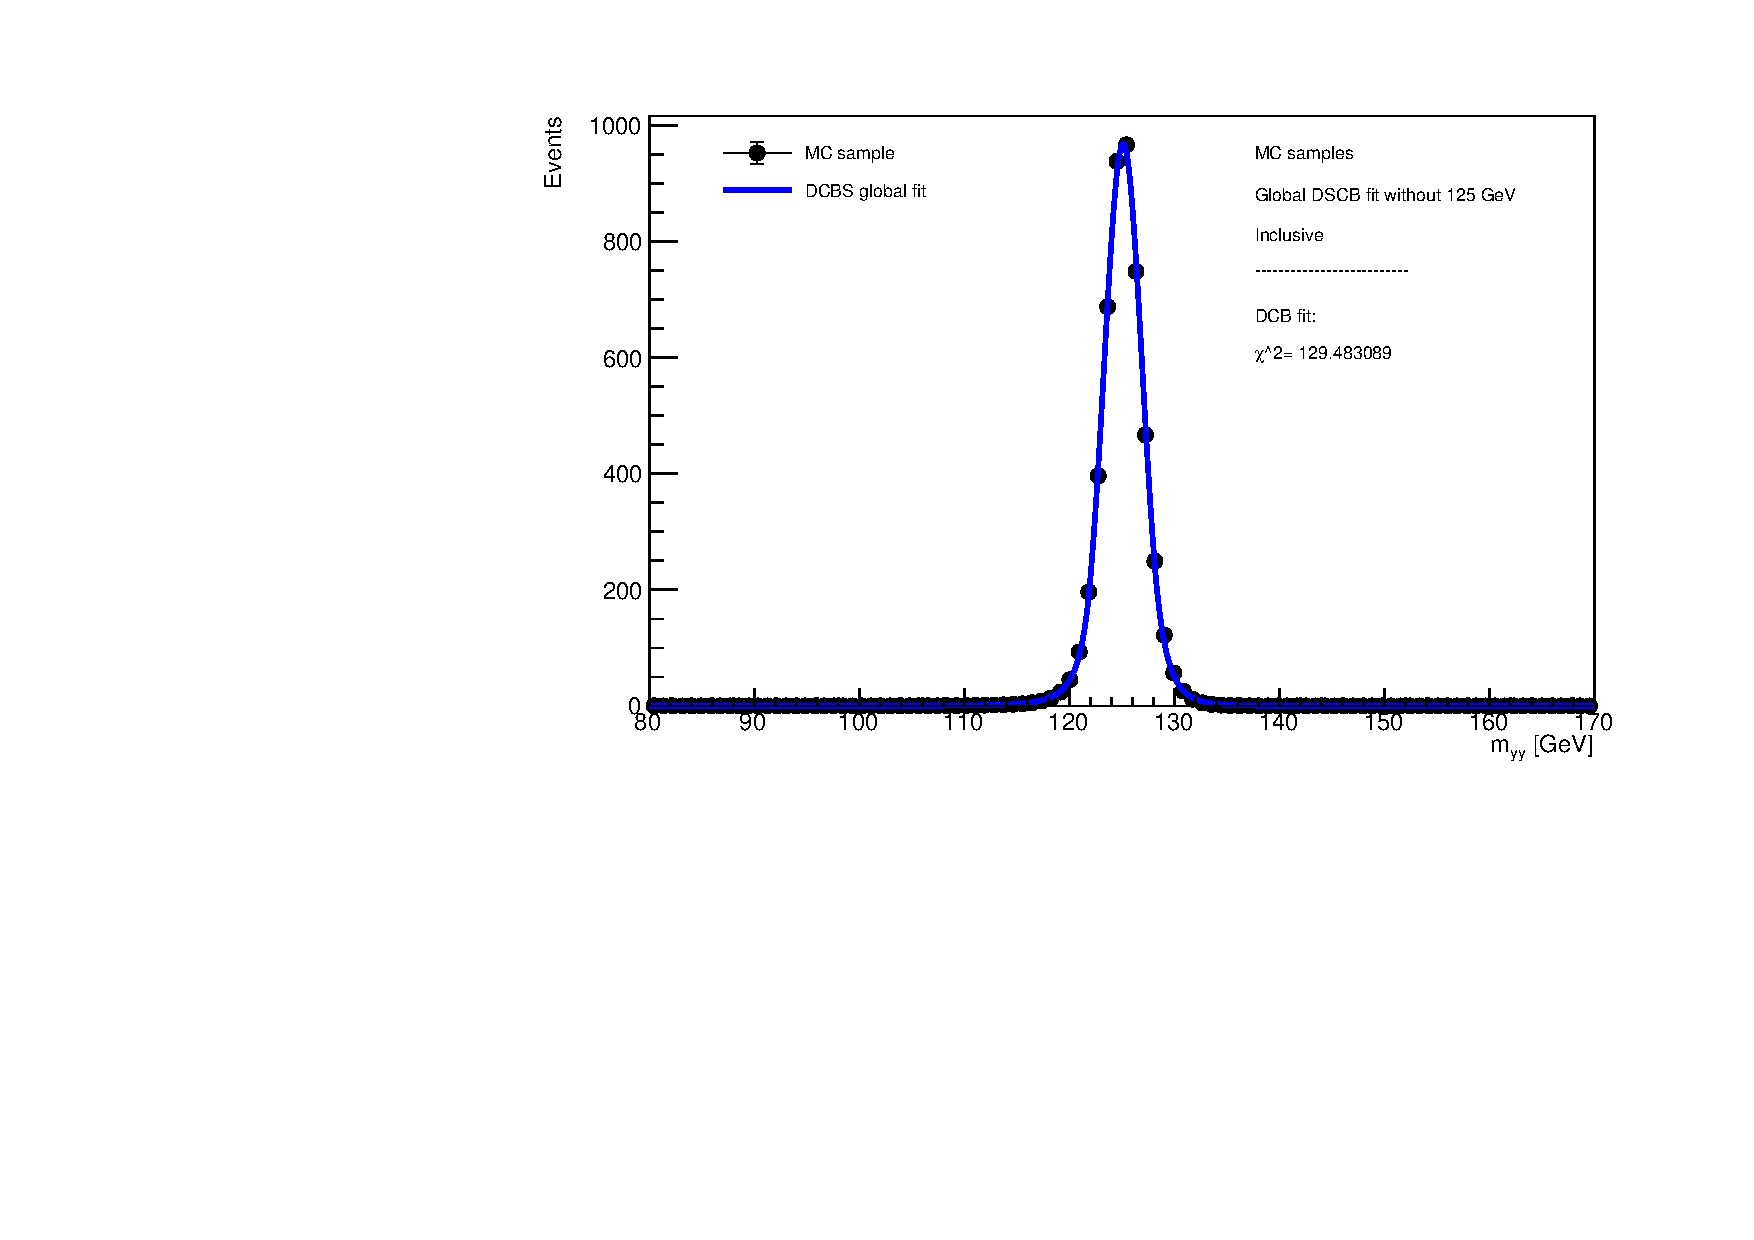
\includegraphics[width=.7\textwidth]{Pres_Images/HGam/myy_125GeV_DCBfit_cutFlow_no125.pdf}
		\end{center}
		\vfill
		\begin{textblock}{}(0.55,0.575)
			
\includegraphics[width=.2\textwidth]{Pres_Images/HGam/white.jpeg}
		\end{textblock}
	\end{frame}
	
	\begin{frame}{Signal yield}
		\vfill
		\begin{scriptsize}
			The signal yield in each category is defined as:
			\begin{center}
				%$yield(mH) = xs^{fit}(mH) \cdot eff^{fit}_{cat}(mH) \cdot br^{fit}(mH) \cdot LumiRun2$
				$yield(mH) = xs_{fid}^{fit}(mH) \cdot C_{X\ \ cat}^{fit}(mH) \cdot br^{fit}(mH) \cdot LumiRun2$
			\end{center}
			\begin{itemize}
				\item $xs_{fid}^{fit}(mH) = 501.988751\cdot\exp(-0.025130\cdot m_{H} + 0.000043\cdot m_{H}^2) \cdot A_X^{fit}(mH)$;
				\item $A_X^{fit}(mH) = 0.264211 + 0.001712\cdot m_H$ 
				\item $br^{fit}(mH) = 0.000120\cdot\exp(64.543706\cdot m_{H} + 806.563546\cdot m_{H}^2)$;
				\item $C^{fit}_{X\ cat}(mH) = A^{cat} + B^{cat}\cdot m_{H}$ $\Leftarrow$ Using only \textit{ggF} MC samples.
				
			\end{itemize}
		\end{scriptsize}
		
		\vspace{.1cm}
		\centering
		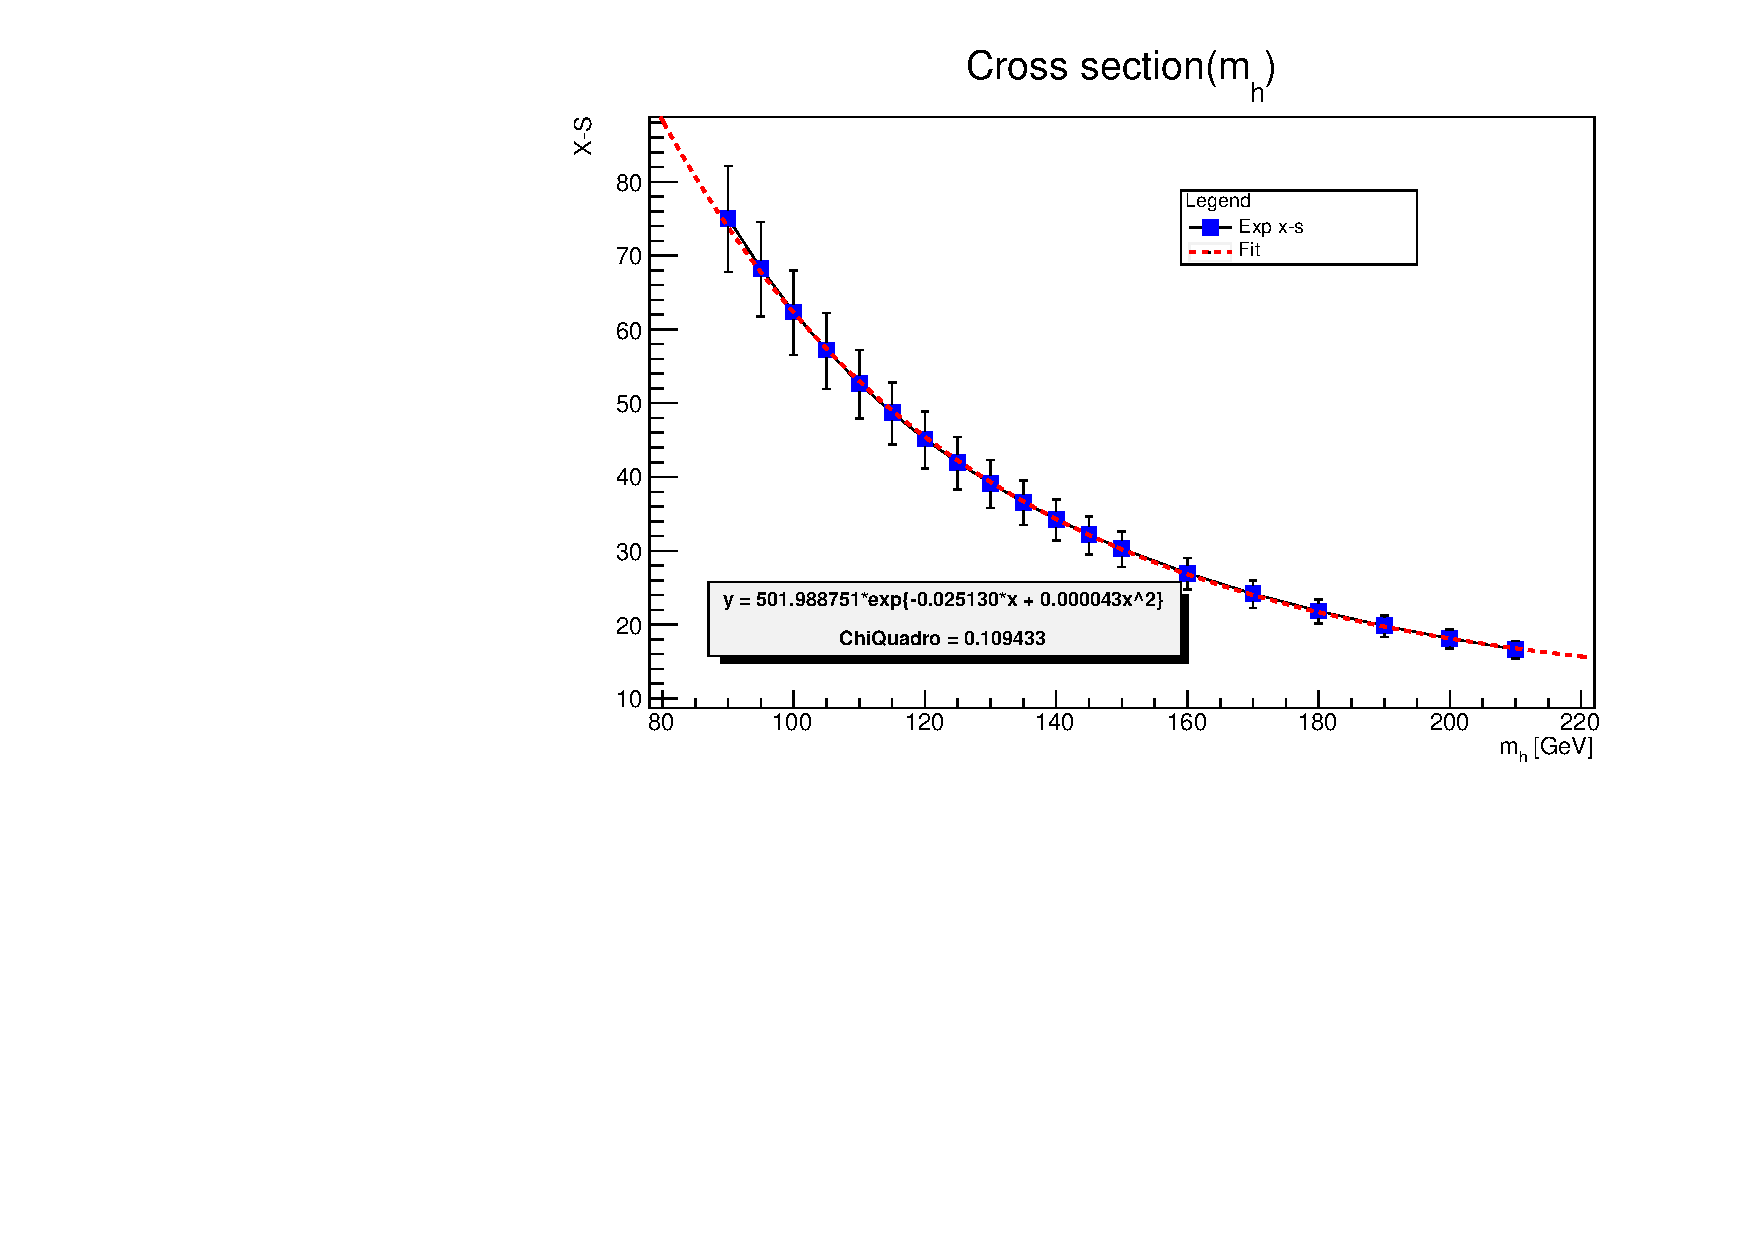
\includegraphics[width=.3\textwidth]{Pres_Images/HGam/x_section_fit.pdf}
		\includegraphics[width=.3\textwidth]{Pres_Images/HGam/ax_linear_fit.pdf}\\
		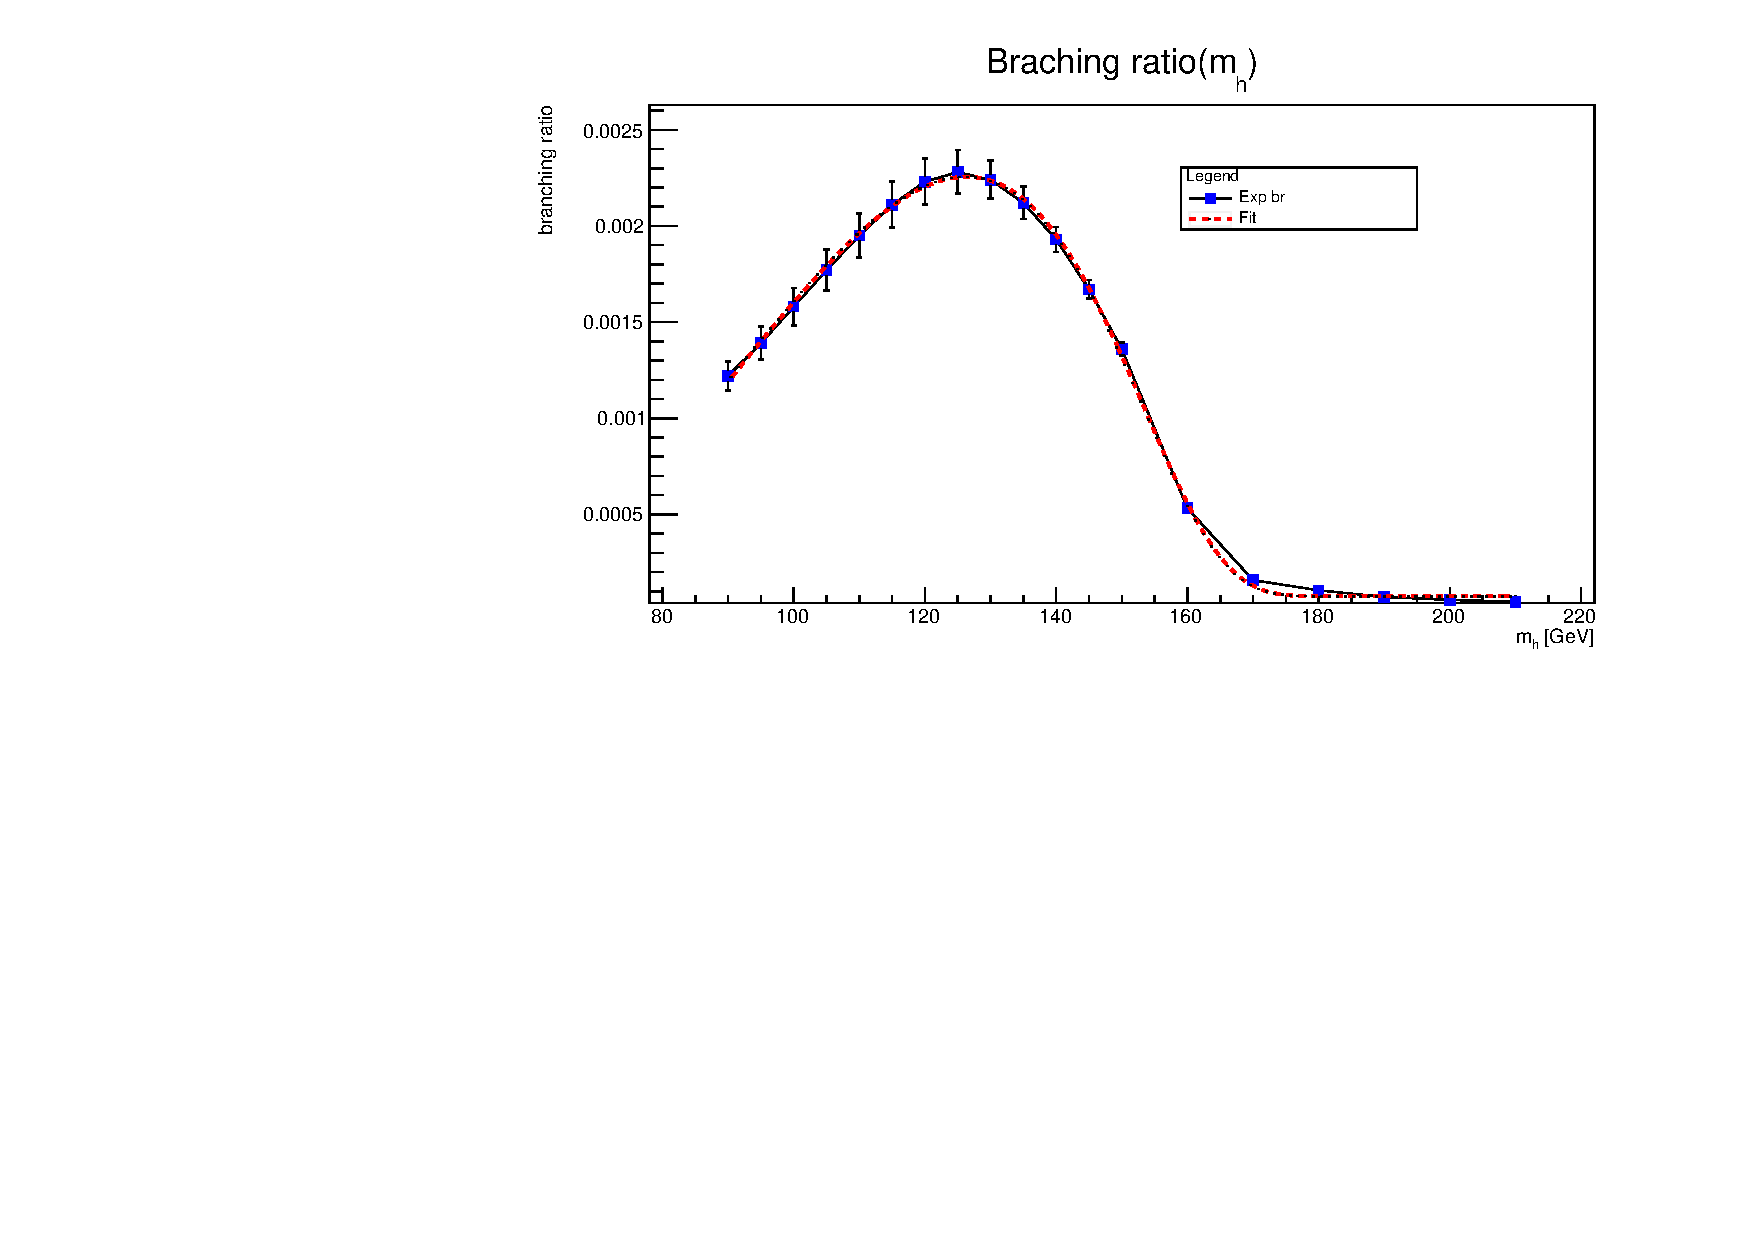
\includegraphics[width=.3\textwidth]{Pres_Images/HGam/br_fit.pdf}
		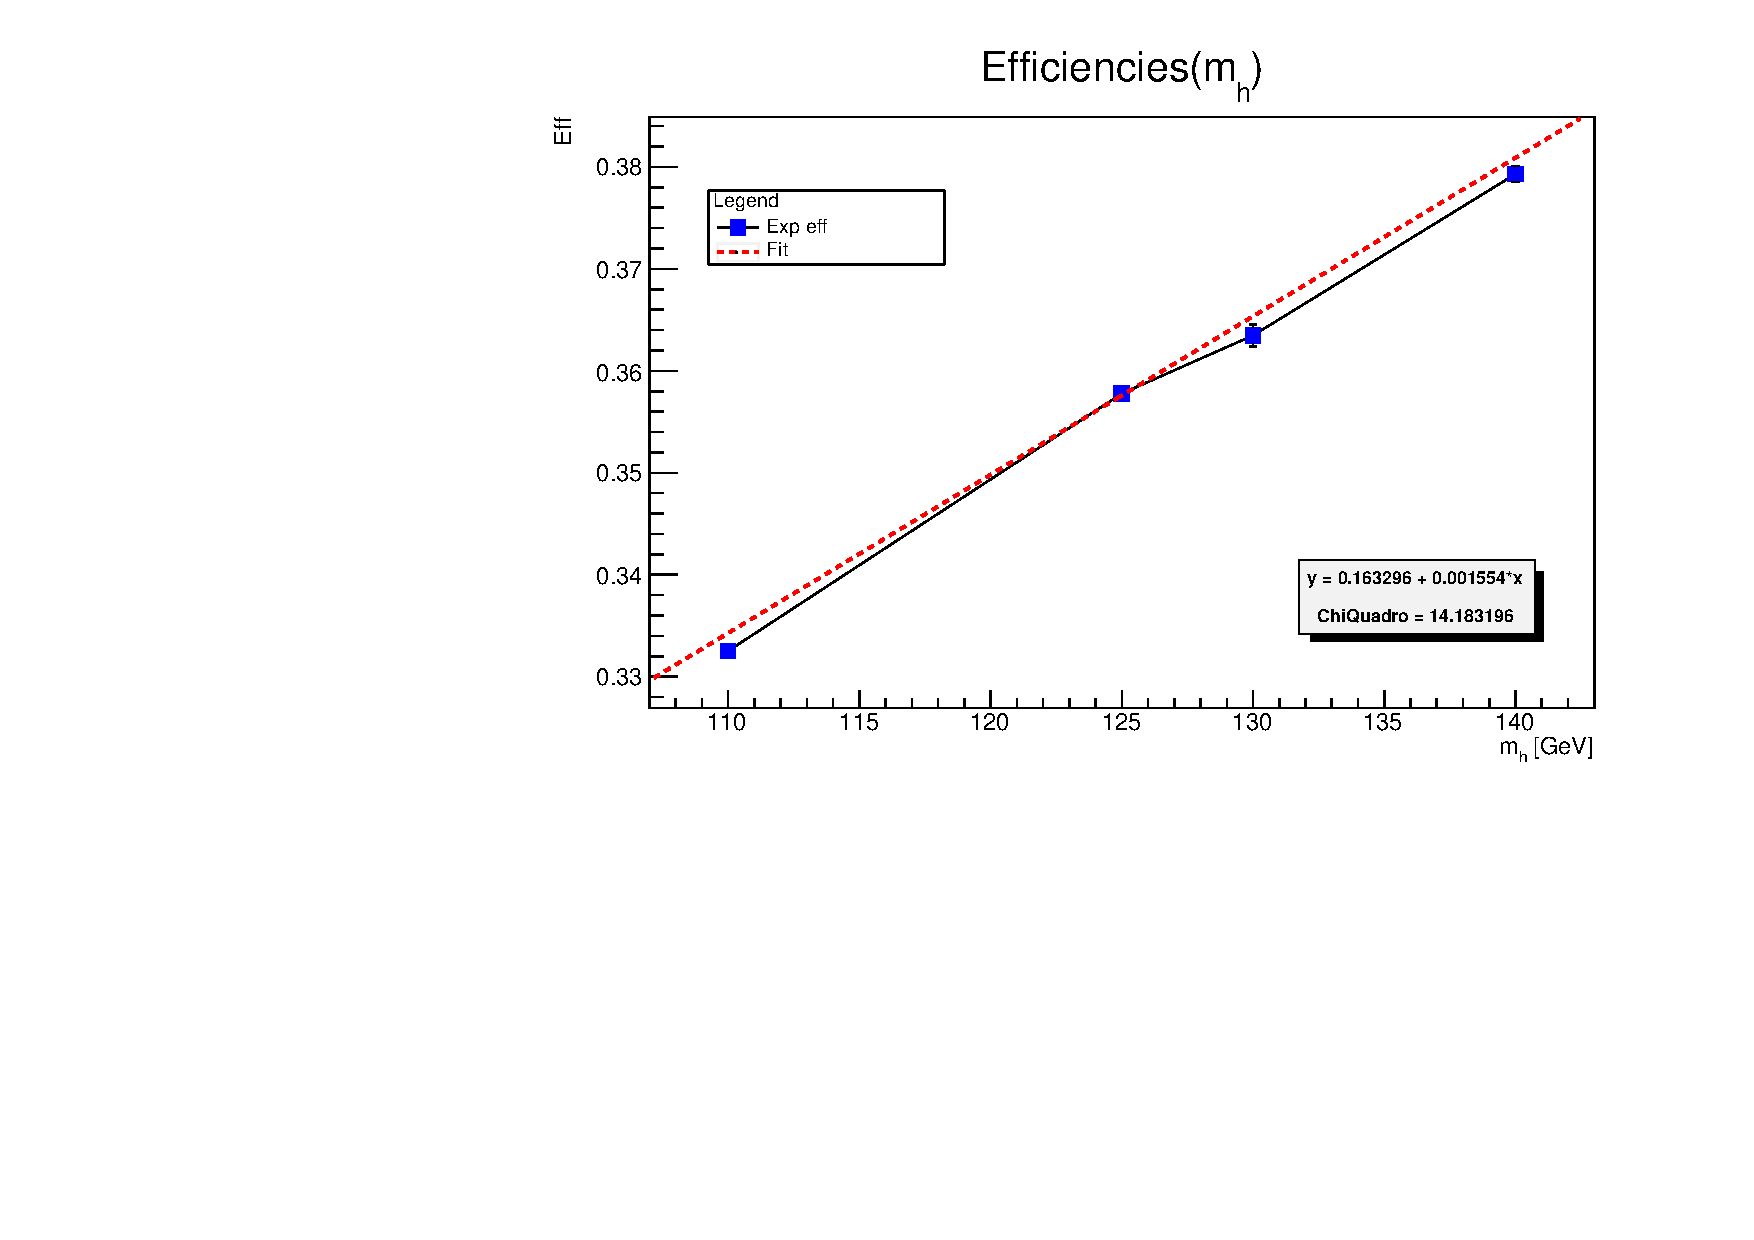
\includegraphics[width=.3\textwidth]{Pres_Images/HGam/efficiencies_fit_1.pdf}
		
		
		\vfill
	\end{frame}
	
	\begin{frame}{Signal yield}
		\vfill
		\begin{center}
			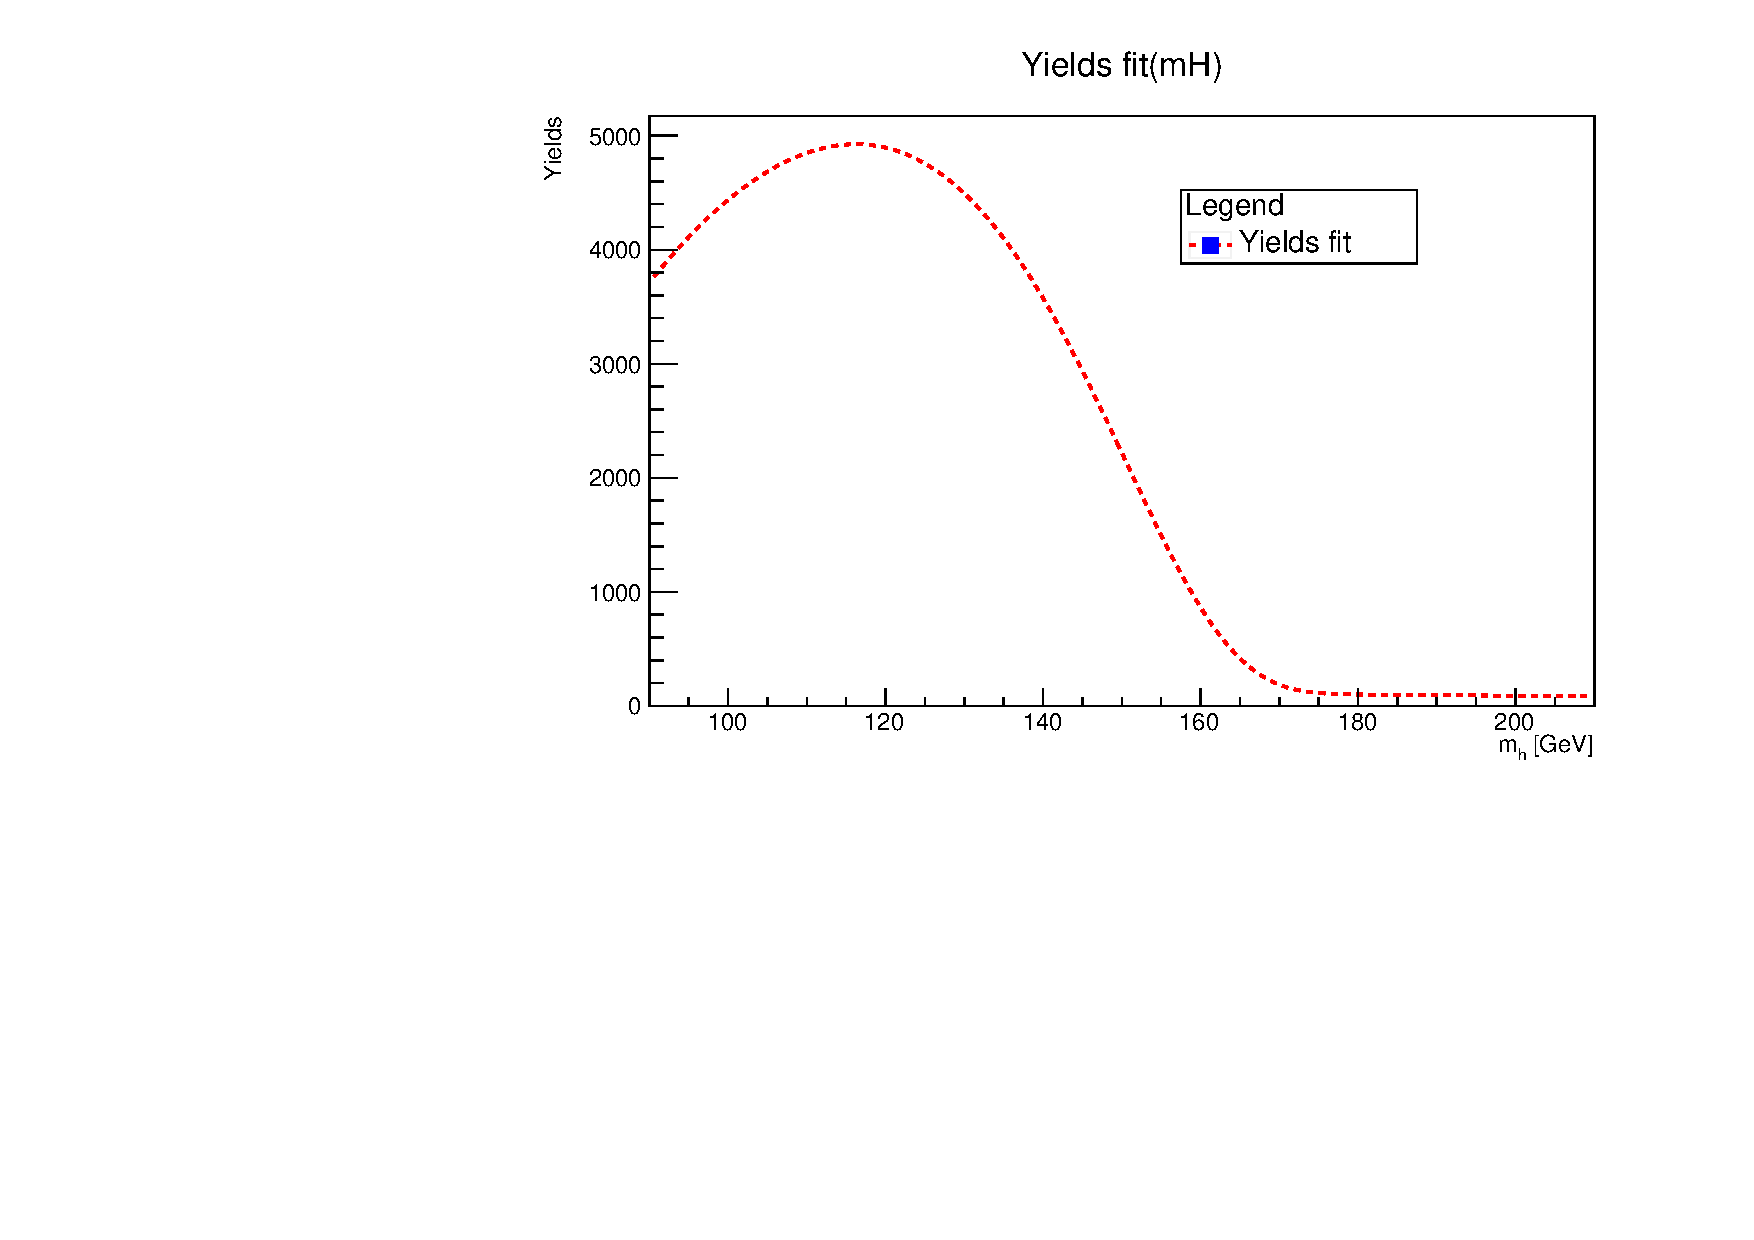
\includegraphics[width=.9\textwidth]{Pres_Images/HGam/check_yields.pdf}
		\end{center}
		\begin{textblock}{1}(0.55,0.45)
			$\int L = 139\ fb^{-1}$\\
			Inclusive
		\end{textblock}
		\vfill
	\end{frame}
	
	\begin{frame}{Background model}
		\vfill
		\begin{itemize}
			\item The background in each category is described by a smoothly falling function whose normalization and shape parameters will be determined from data;
			\item A simple exp(poly2) fit is used for the creation of the background model;
			\item The functional form is tested using MC samples.
		\end{itemize}
		\begin{center}
			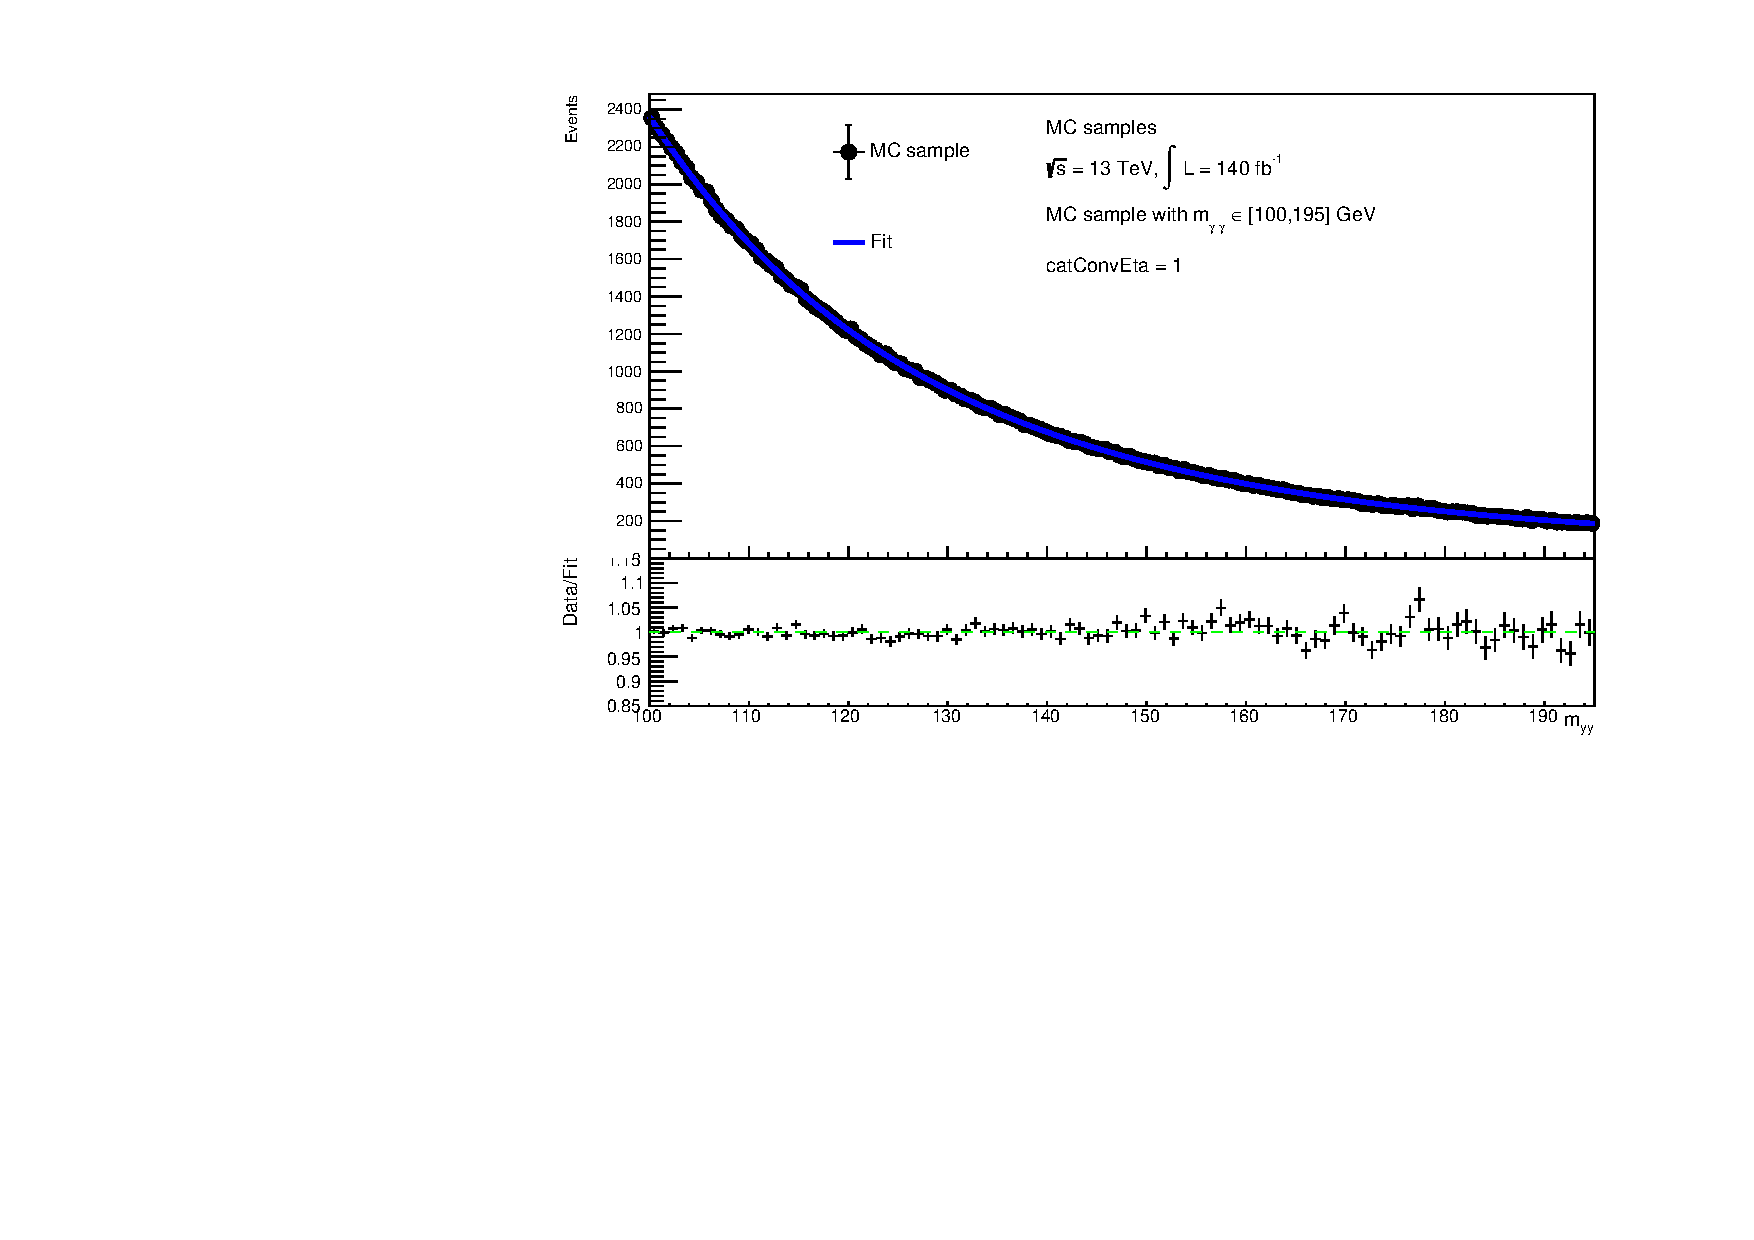
\includegraphics[width=.7\textwidth]{Pres_Images/HGam/bkg_100_195GeV_fit_catConvEta_1.pdf}
		\end{center}
		\vfill
	\end{frame}

		\begin{frame}{Sig/$\sqrt{Bkg}$ comp}
		\vfill
		\begin{table}[tbp]
			\centering
			\begin{tabular}{lcccc}
				\toprule[1.5pt]
				cat & 110 GeV	& 125 GeV	& 130 GeV	& 140 GeV	\\
				\midrule
				inclusive & 9.012 & 11.947 & 11.865 & 9.277 	\\ 
				1 & 4.583 & 6.100 & 6.088 & 4.817 	\\
				2 & 4.572 & 6.006 & 6.052 & 4.714 	\\
				3 & 2.268 & 2.909 & 2.856 & 2.240 	\\
				4 & 3.416 & 4.582 & 4.532 & 3.618 	\\
				5 & 4.354 & 5.788 & 5.724 & 4.513 	\\
				6 & 2.661 & 3.451 & 3.415 & 2.683 	\\
				Sum & 9.207 & 12.171 & 12.117 & 9.544	\\
				\bottomrule[1.5pt]
			\end{tabular}
			\caption{Number of signal and $\sqrt{bkg}$ events ratio in [peak-3$\sigma$,peak+3$\sigma$] GeV interval}
		\end{table}
		\vfill
	\end{frame}

	\begin{frame}{Higgs SM}
		\vfill
		\begin{itemize}
			\item The Higgs SM background component is created merging all 125 GeV SM production modes and fitting this distribution with a DSCB fit;.
		\end{itemize}
		\begin{center}
			\includegraphics[width=.65\textwidth]{Pres_Images/HGam/HSM_fit_catConvEta_1.pdf}
		\end{center}
		\vfill
	\end{frame}
	
	\begin{frame}{Syst unc MC sample}
		\vfill
		Systematic uncertainties are obtained only using h026 MC sample with 125 GeV mass, merging and weighting the three flavours (mc16a, mc16d, mc16e).
		
		\vspace{.5cm}
		\textbf{Folder}:\\ 
		{\small
			/eos/atlas/atlascerngroupdisk/phys-higgs/HSG1/MxAOD/h026/mc16*/PhotonSys/
		}
		
		\vspace{.5cm}
		\textbf{Syst uncertainties}:
		\begin{itemize}
			\item \textcolor{green}{Signal systs} $\to$ used only ggF;
			\item \textcolor{orange}{Higgs SM bkg systs} $\to$ used all prod modes merged;
		\end{itemize} 
		%\begin{itemize}
		%	\item {\scriptsize mc16a.PowhegPy8\_NNLOPS\_ggH125.MxAODPhotonSys.e5607\_s3126\_r9364\_p4180\_h026.root;}
		%	\item {\scriptsize mc16d.PowhegPy8\_NNLOPS\_ggH125.MxAODPhotonSys.e5607\_s3126\_r10201\_p4180\_h026.root;}
		%	\item {\scriptsize mc16e.PowhegPy8\_NNLOPS\_ggH125.MxAODPhotonSys.e5607\_s3126\_r10724\_p4180\_h026.root;}
		%end{itemize}
		\vfill
	\end{frame}
	
	\begin{frame}{Yield systematic uncertainties}
		\vfill 
		The systematic uncertainties inserted in signal model are:
		\begin{itemize}
			\item Yield $\rightarrow$ $\pm1\sigma$ variations:
			\begin{itemize}
				{\small
					\item ATLAS\_EG\_RESOLUTION\_ALL;
					%\item ATLAS\_EG\_SCALE\_AF2;
					\item ATLAS\_EG\_SCALE\_ALL;
					\item ATLAS\_PH\_EFF\_ID\_Uncertainty;
					\item ATLAS\_PH\_EFF\_ISO\_Uncertainty;
					\item ATLAS\_PH\_EFF\_TRIGGER\_Uncertainty;
					\item ATLAS\_PRW\_DATASF;}
			\end{itemize}
		\end{itemize}
		\vfill
	\end{frame}
	
	\begin{frame}{Yield systematic uncertainties (ggF)}
		\vfill
		\centering
		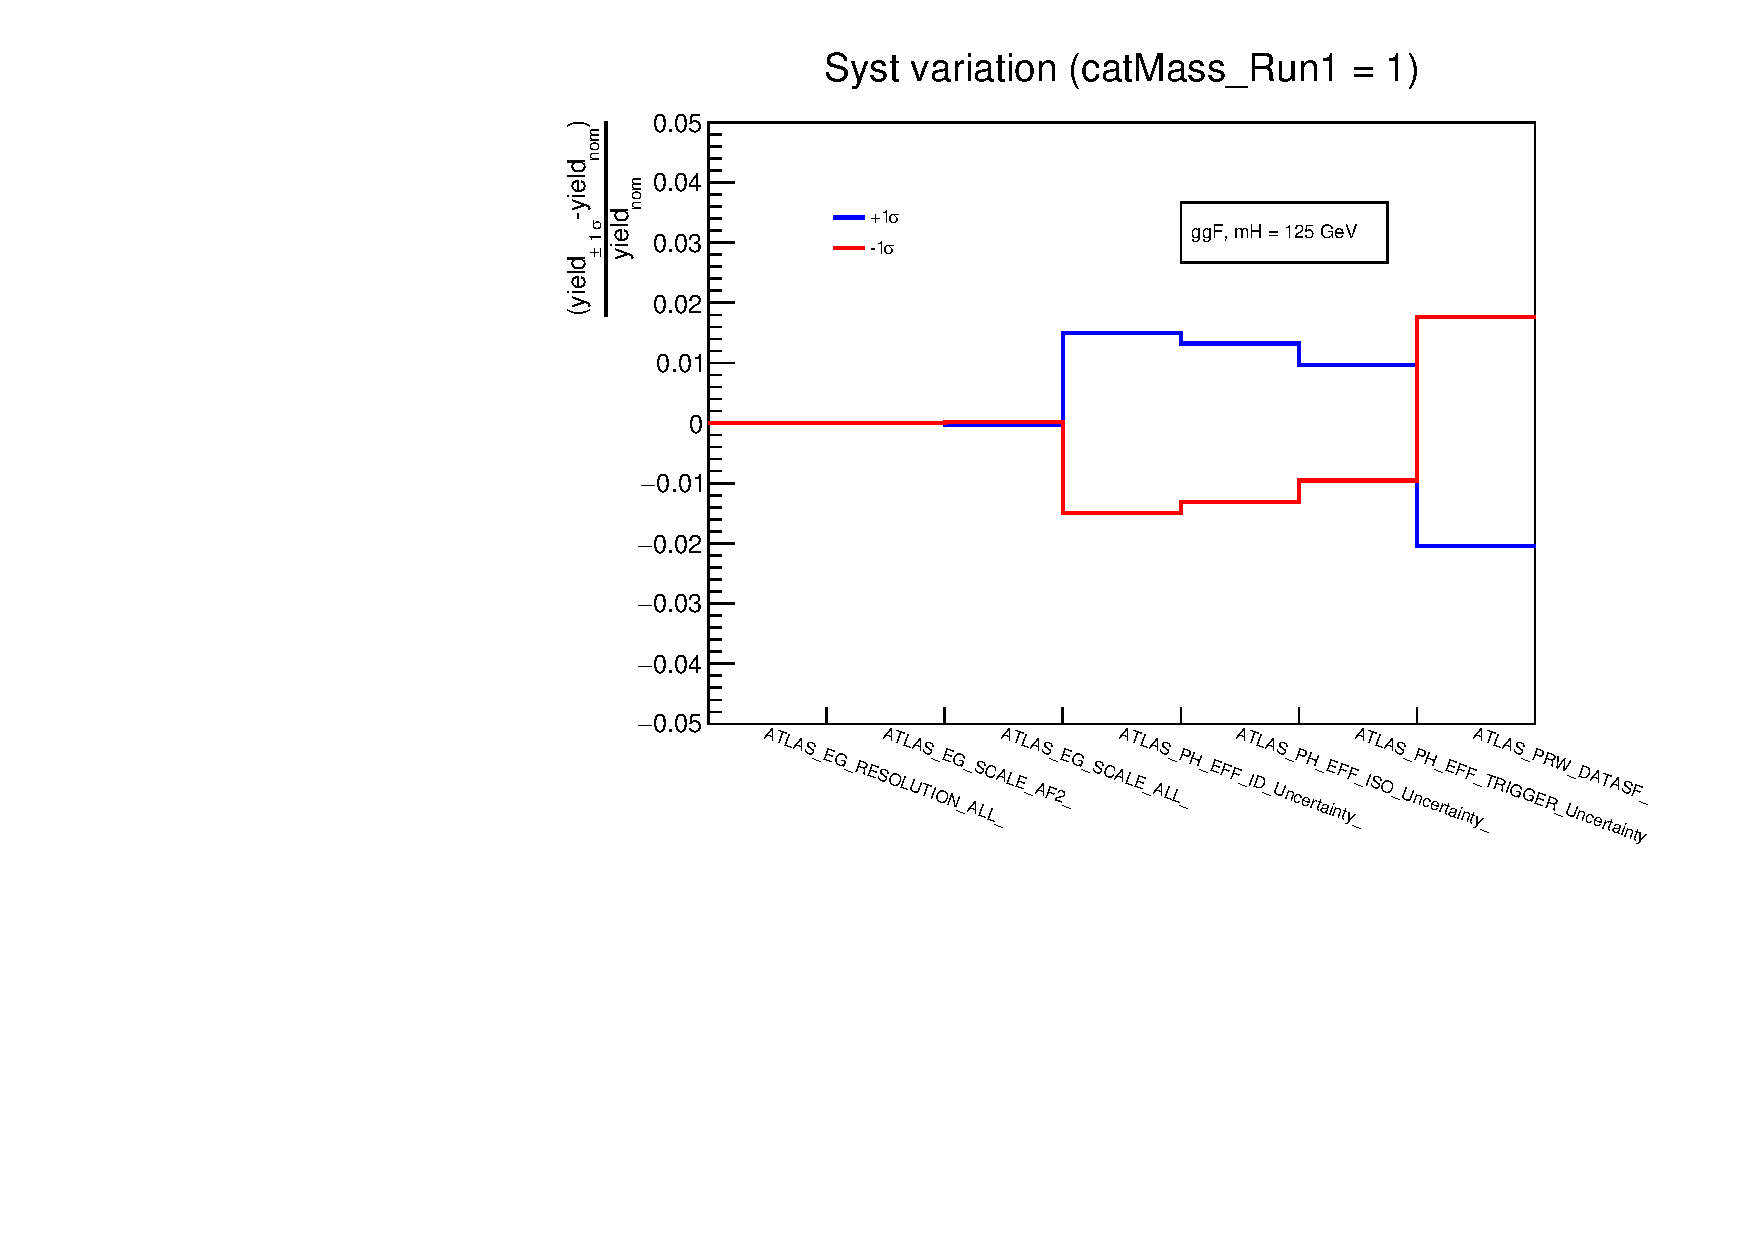
\includegraphics[width=.325\textwidth]{Pres_Images/HGam/Syst/var_cat_1.pdf}
		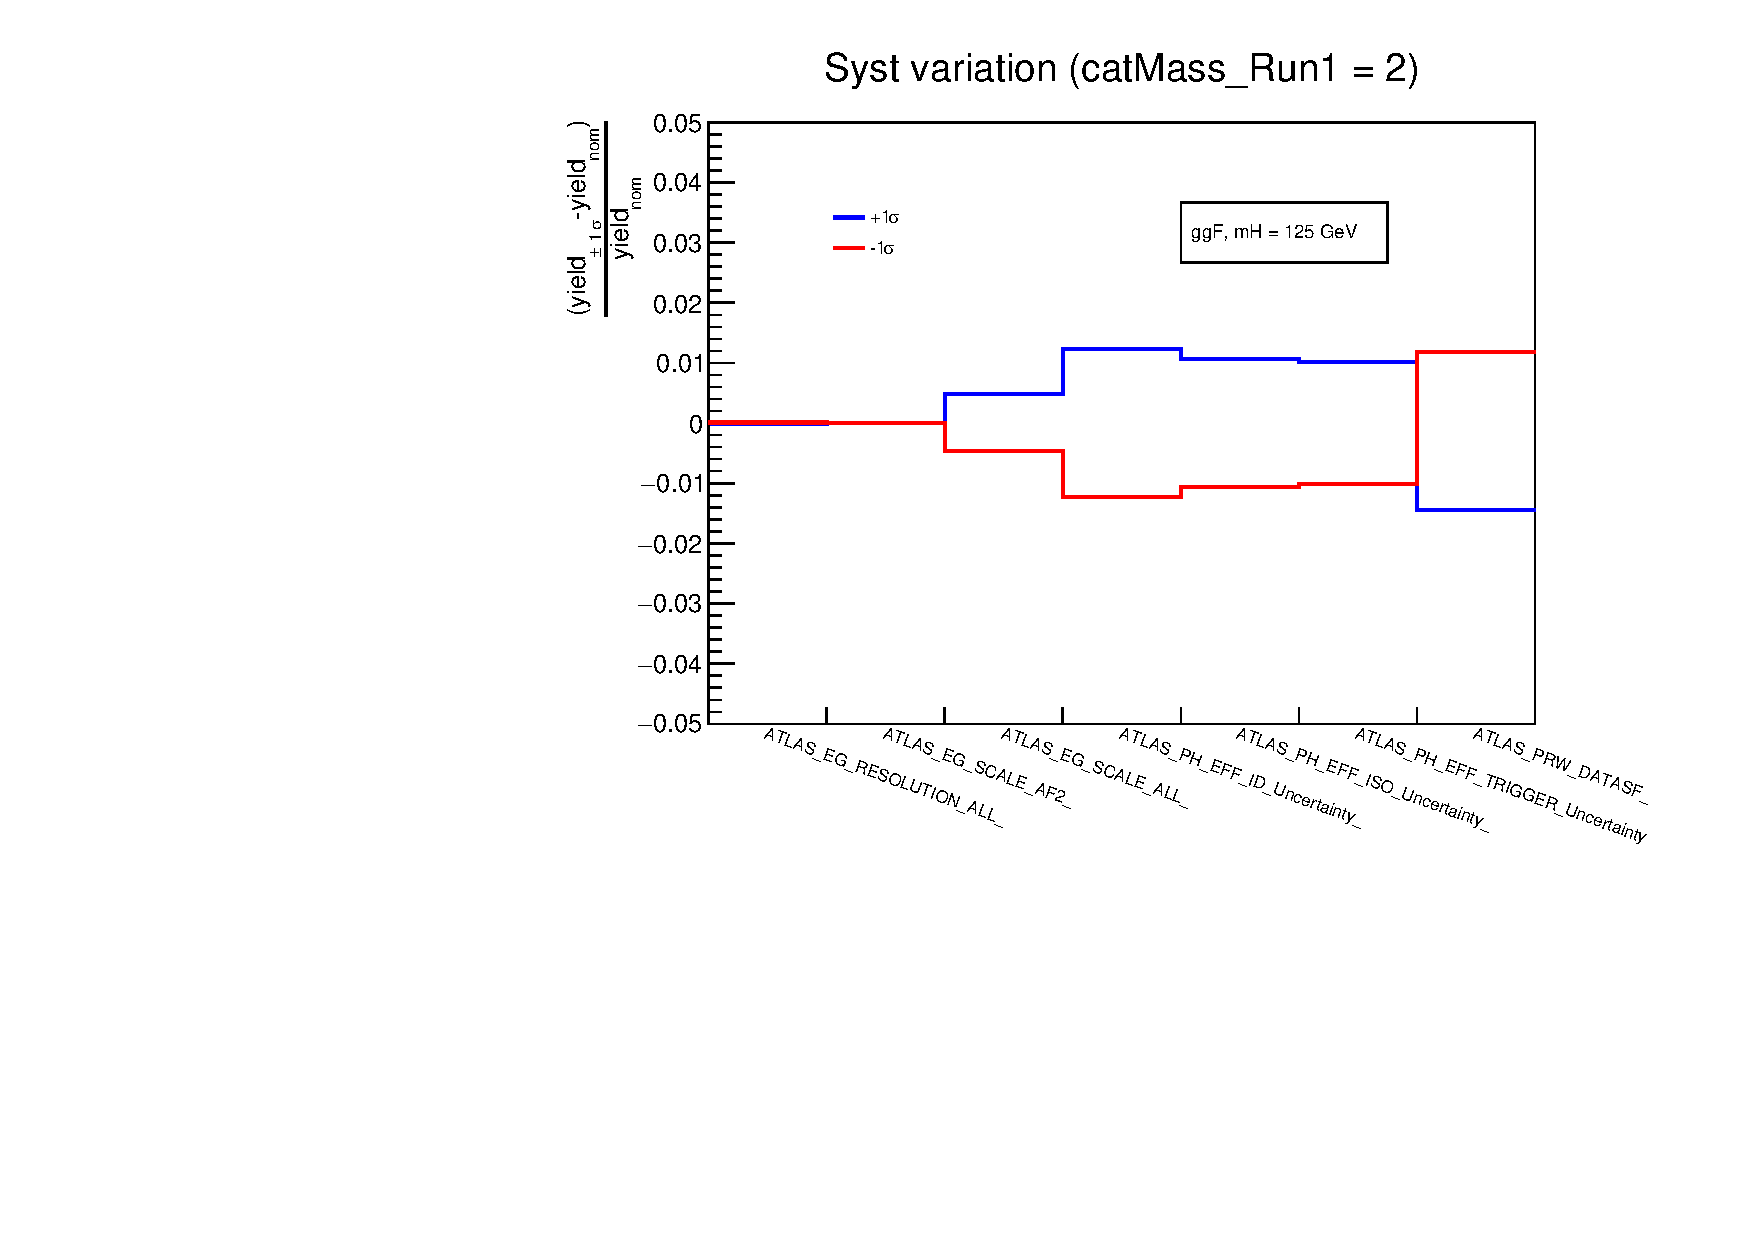
\includegraphics[width=.325\textwidth]{Pres_Images/HGam/Syst/var_cat_2.pdf}
		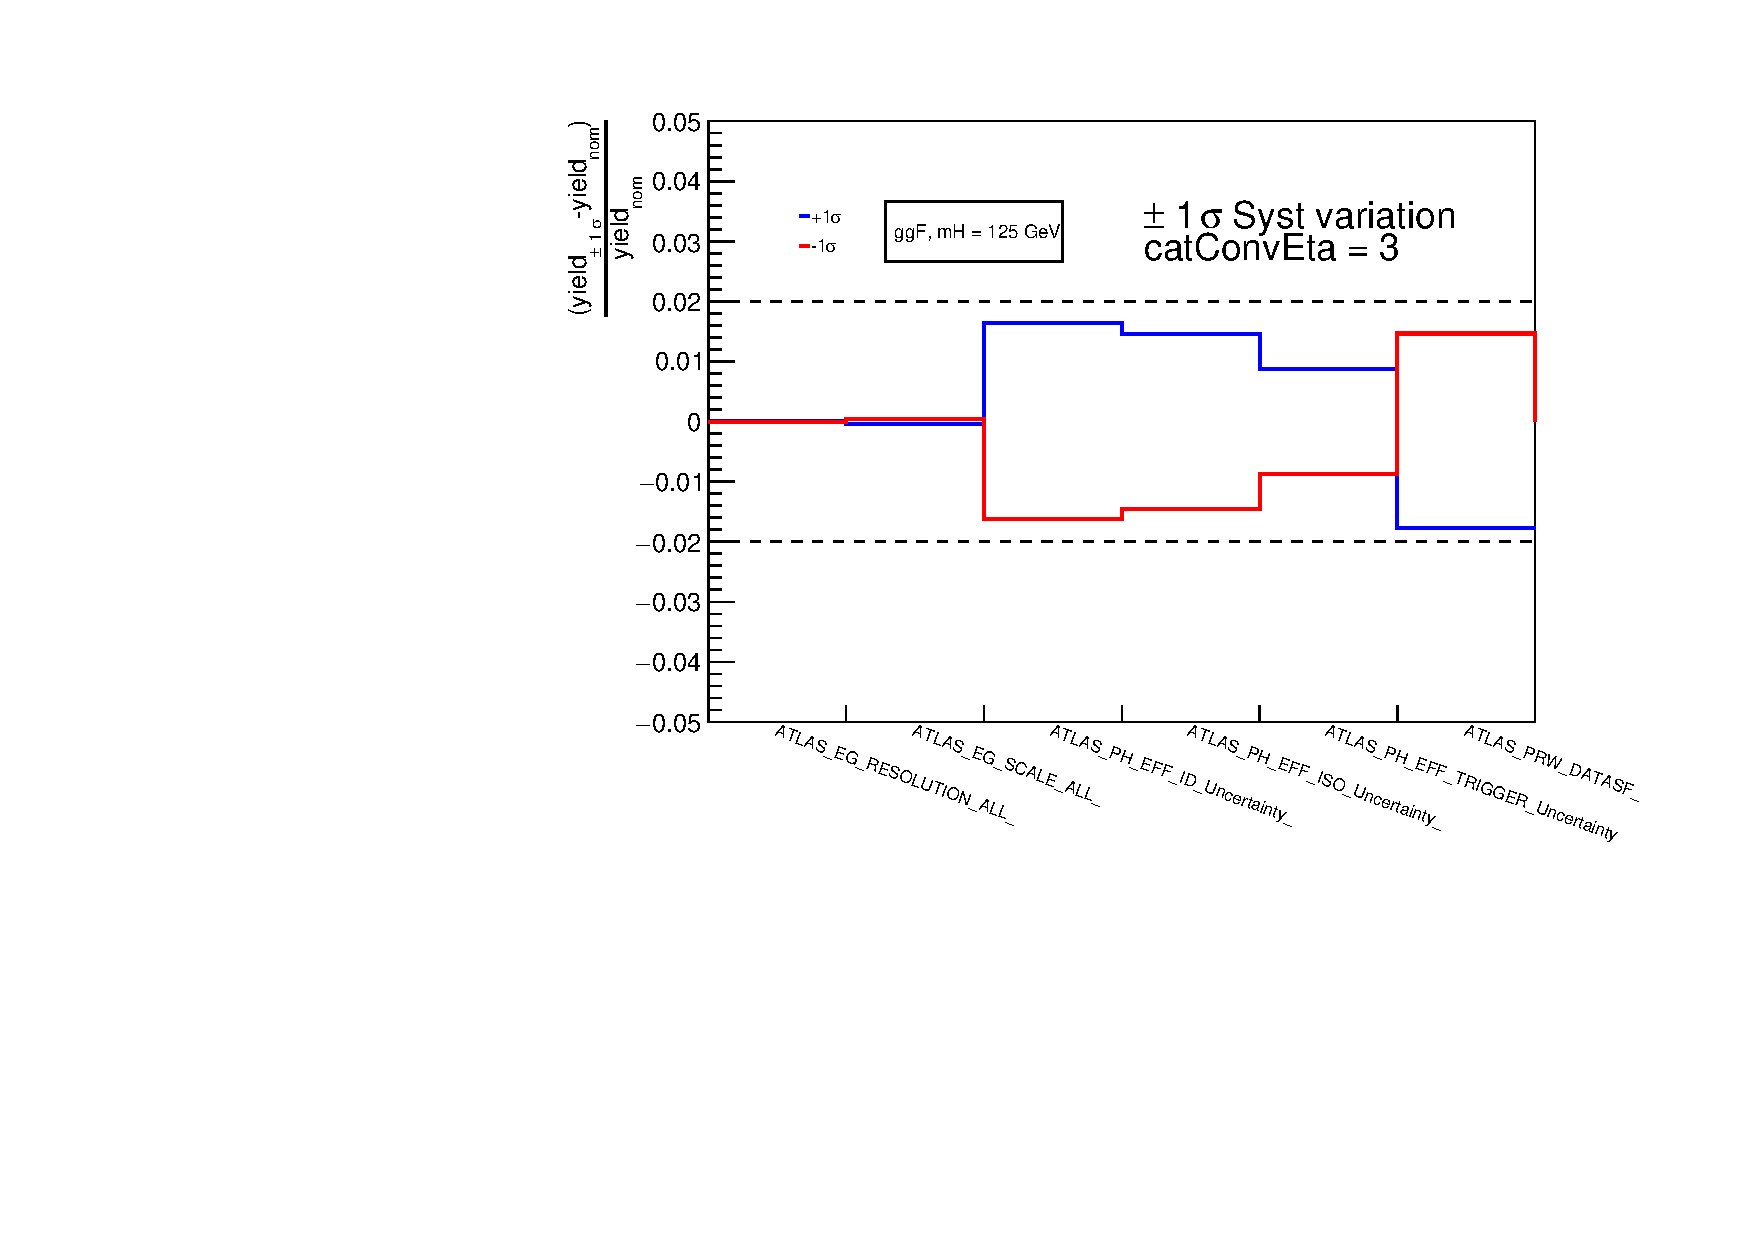
\includegraphics[width=.325\textwidth]{Pres_Images/HGam/Syst/var_cat_3.pdf}
		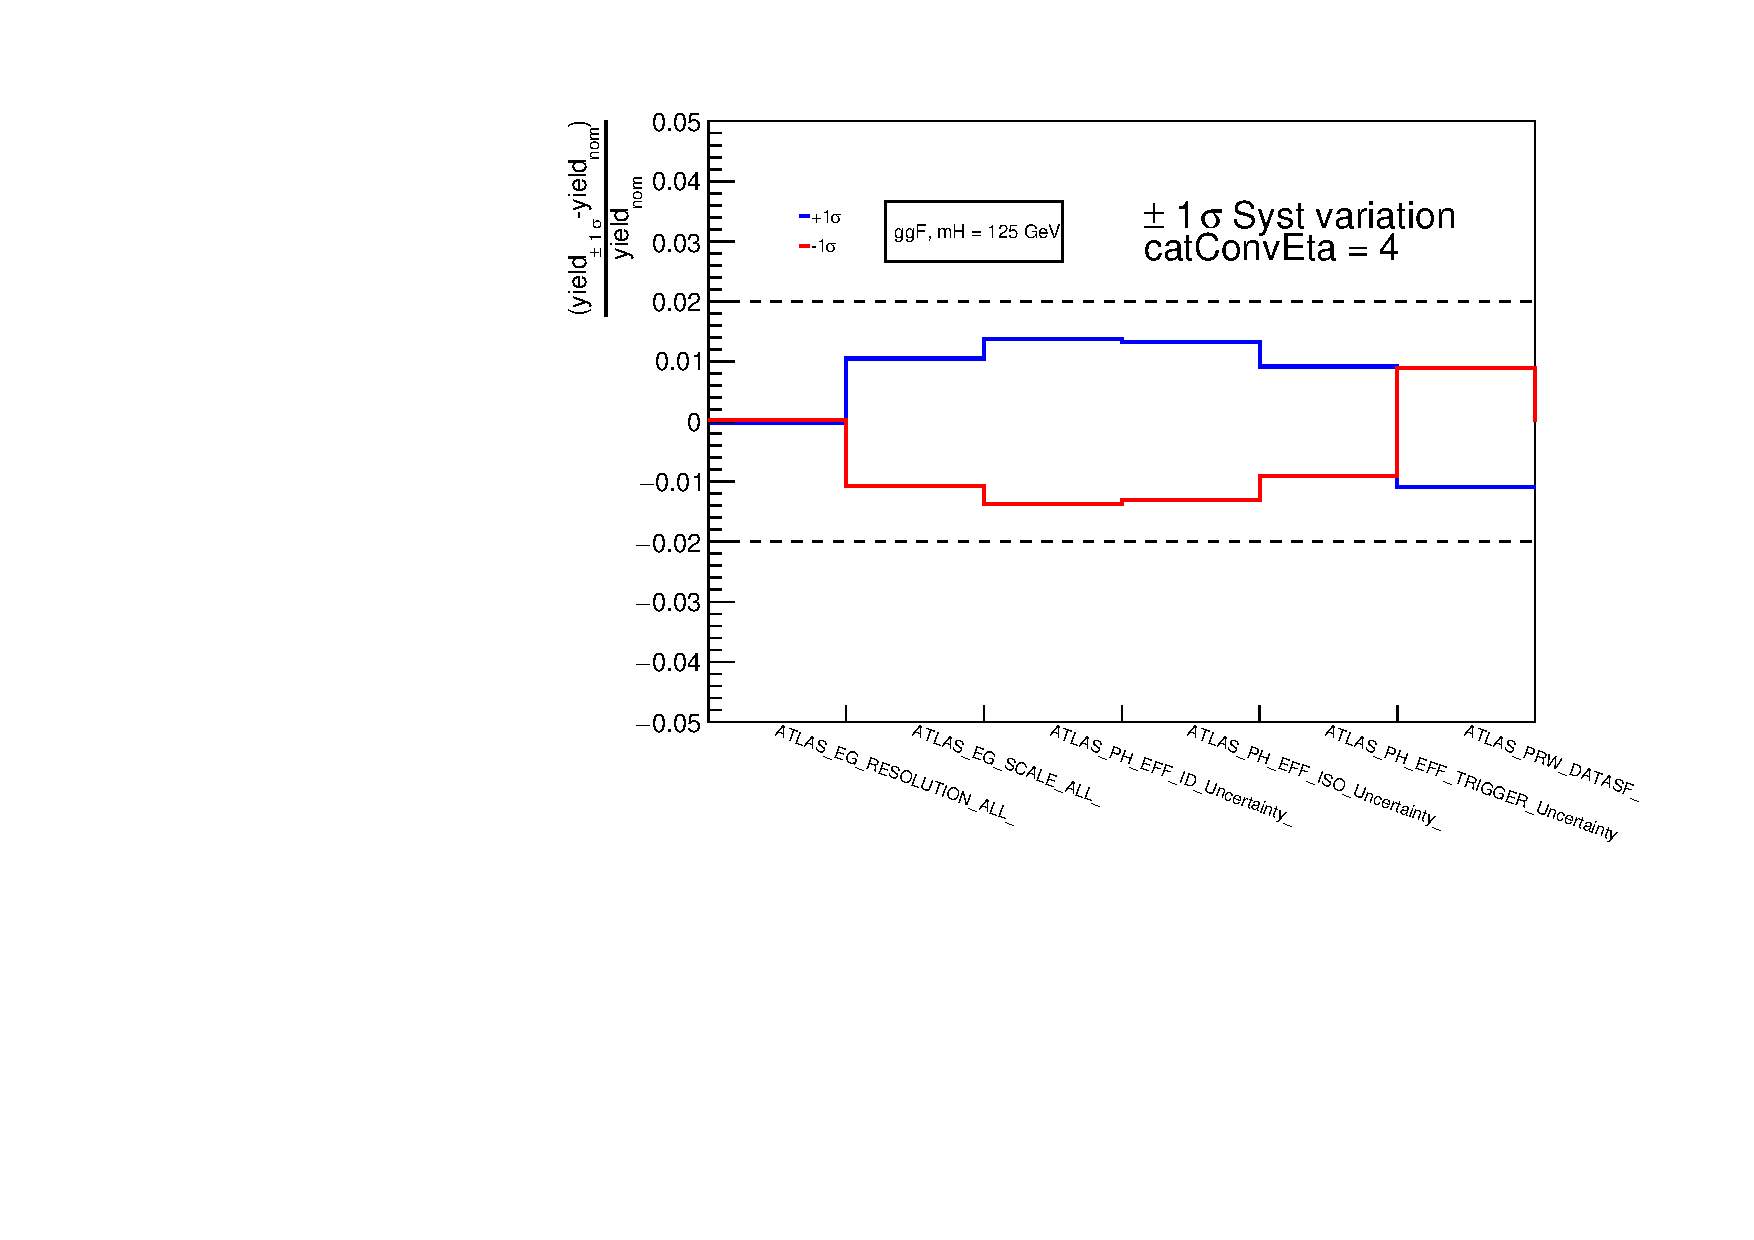
\includegraphics[width=.325\textwidth]{Pres_Images/HGam/Syst/var_cat_4.pdf}
		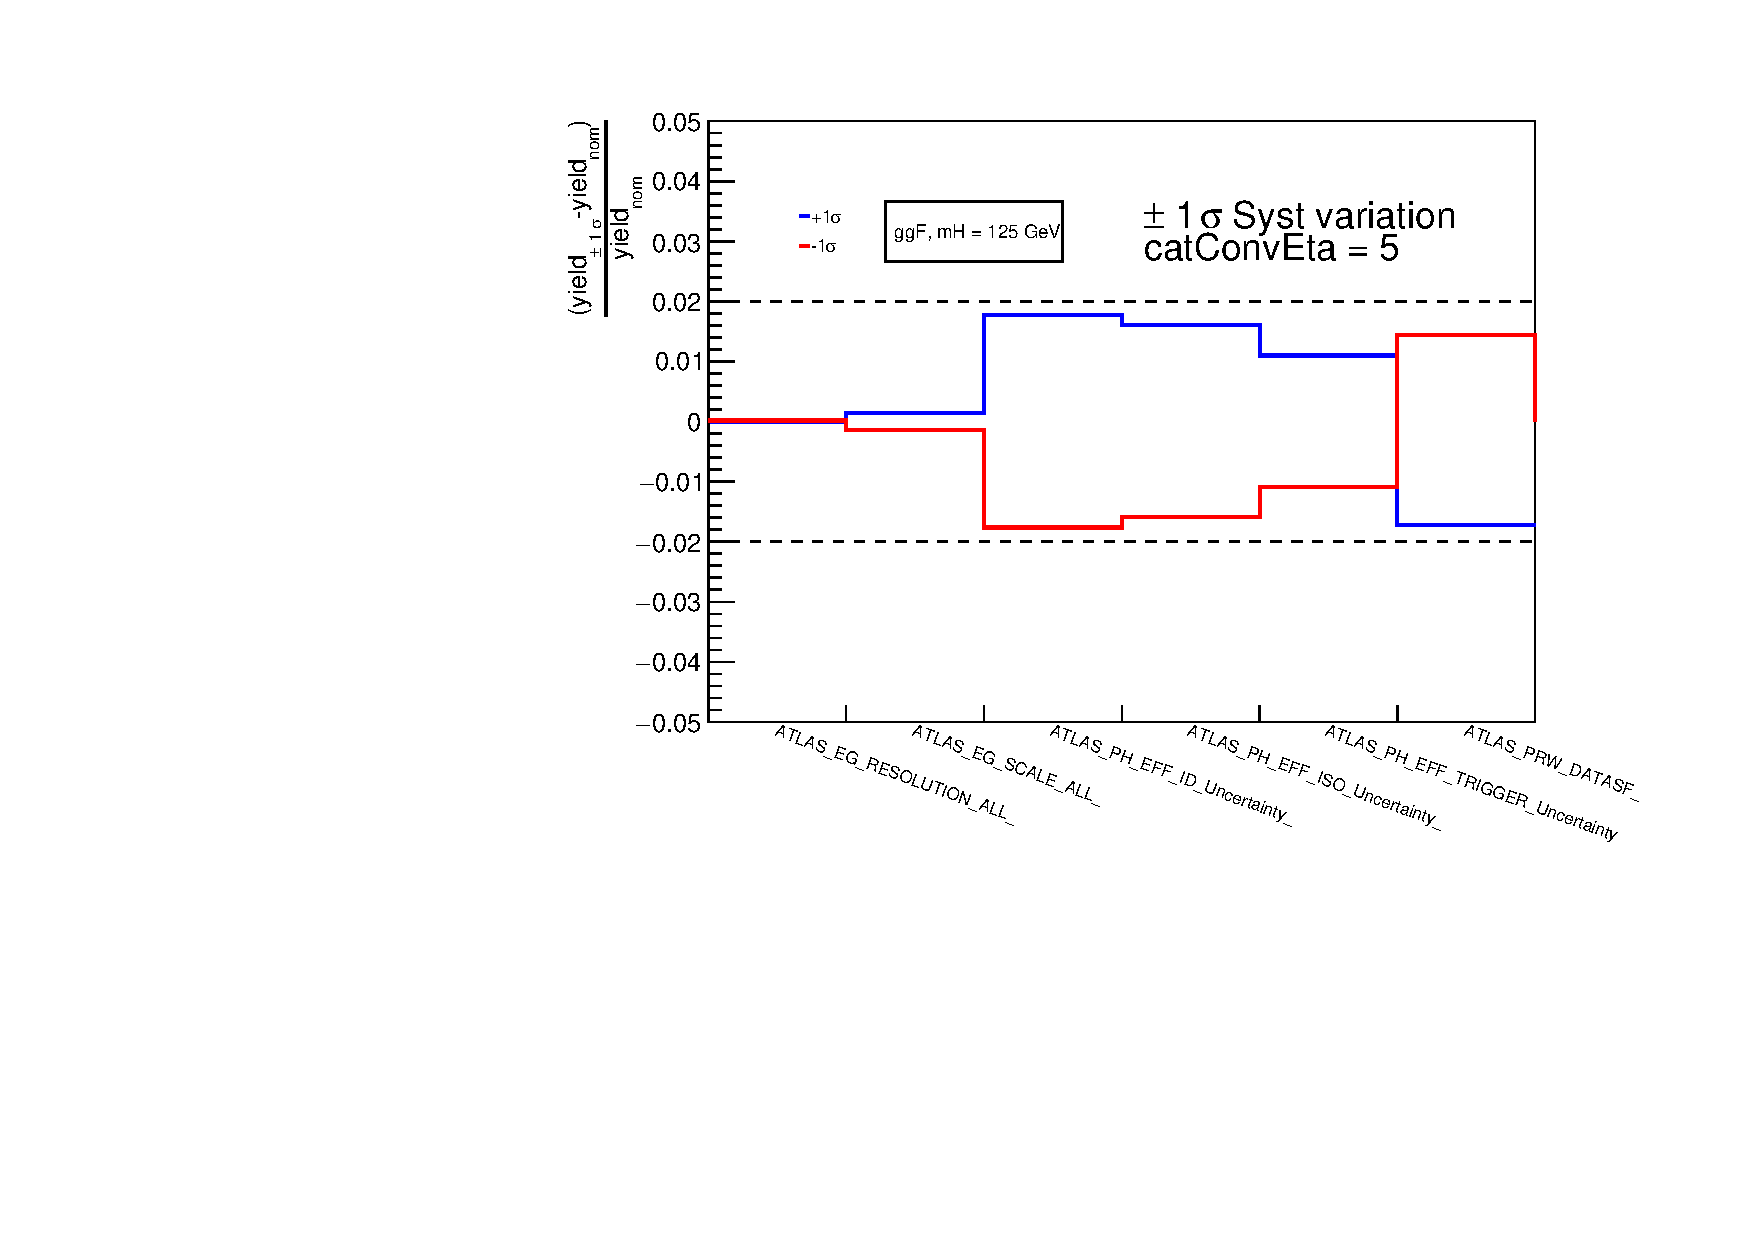
\includegraphics[width=.325\textwidth]{Pres_Images/HGam/Syst/var_cat_5.pdf}
		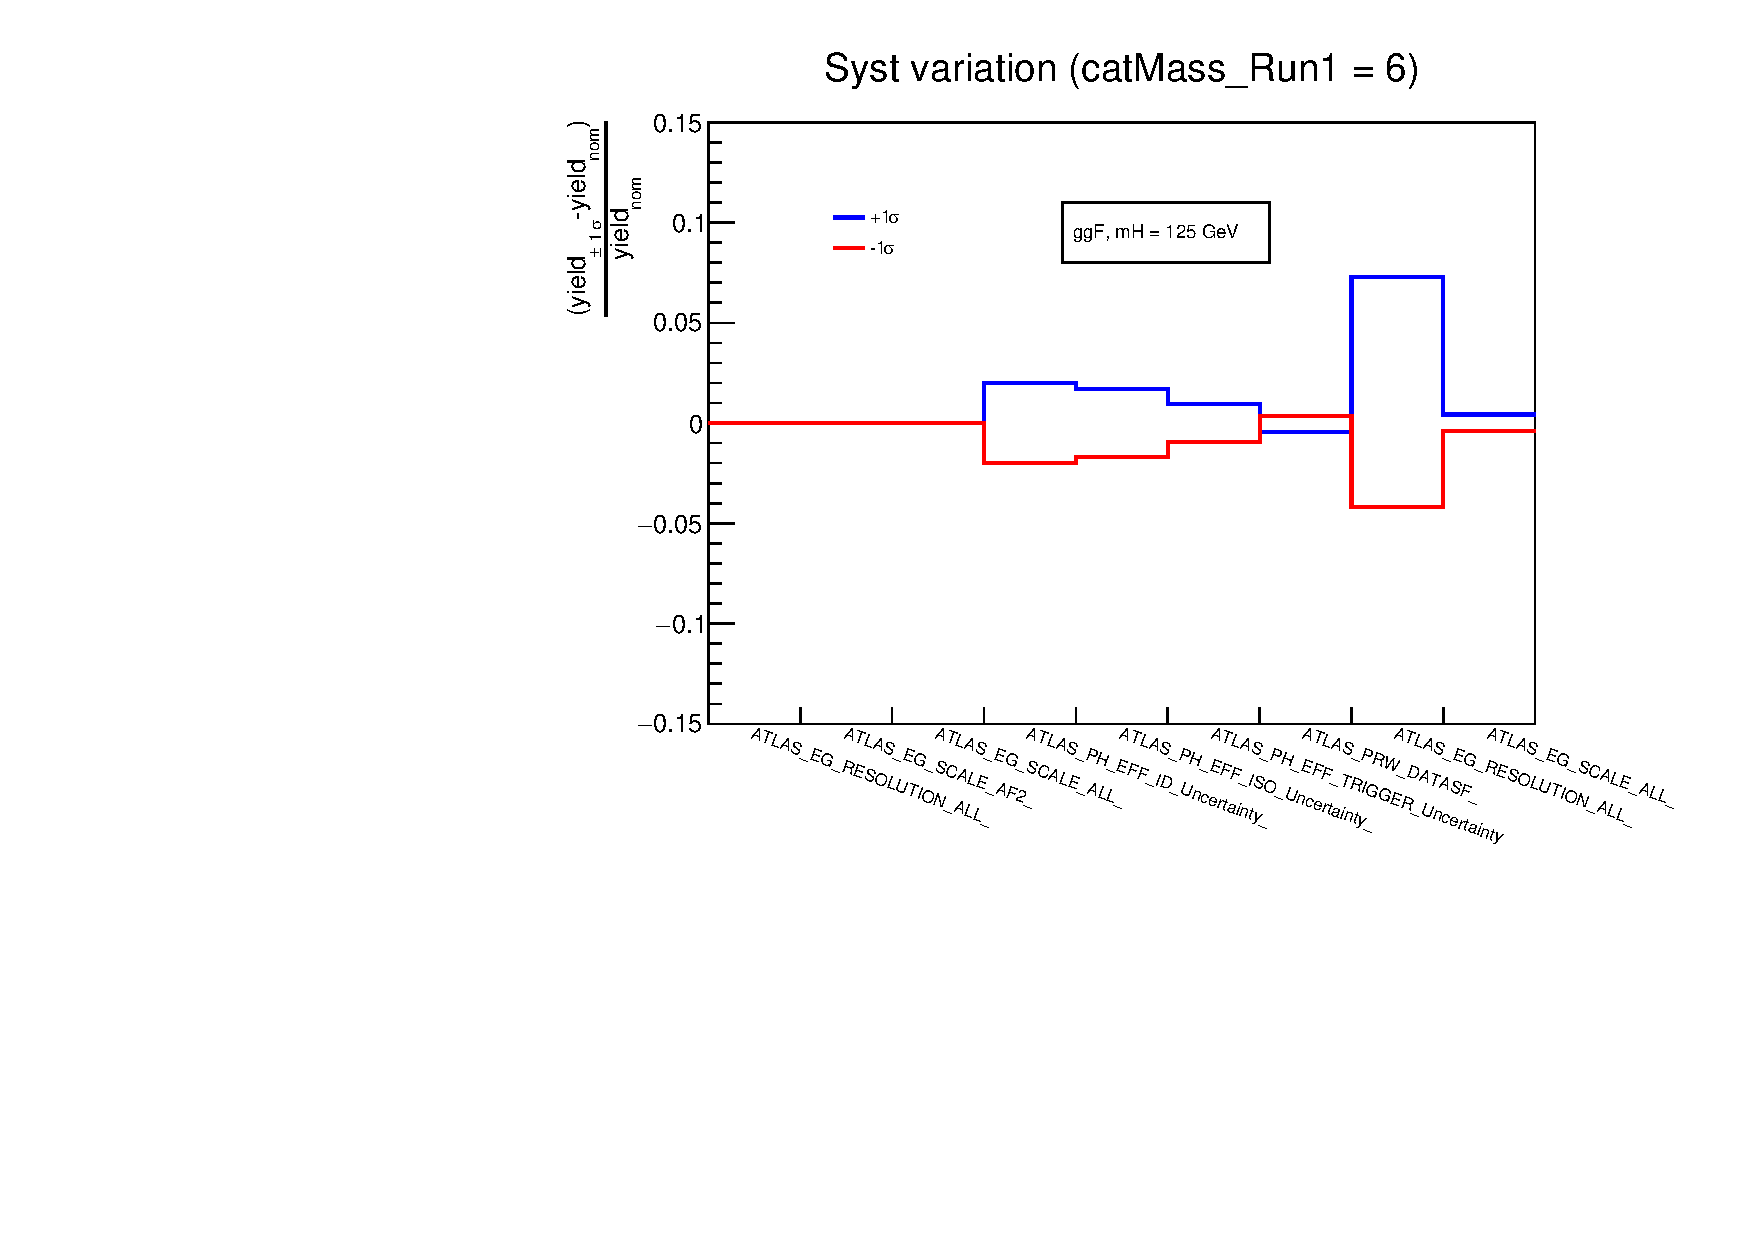
\includegraphics[width=.325\textwidth]{Pres_Images/HGam/Syst/var_cat_6.pdf}
		\vfill
	\end{frame}
	
	\begin{frame}{Shape systematic uncertainties (ggF)}
		\vfill
		The Shape systematic uncertainties inserted in signal model are:
		\begin{itemize}
			\item Shape $\rightarrow$ $\pm1\sigma$ variations:
			\begin{itemize}
				\item ATLAS\_EG\_RESOLUTION\_ALL;
				\item ATLAS\_EG\_SCALE\_ALL;
			\end{itemize}
		\end{itemize}
		\begin{center}
			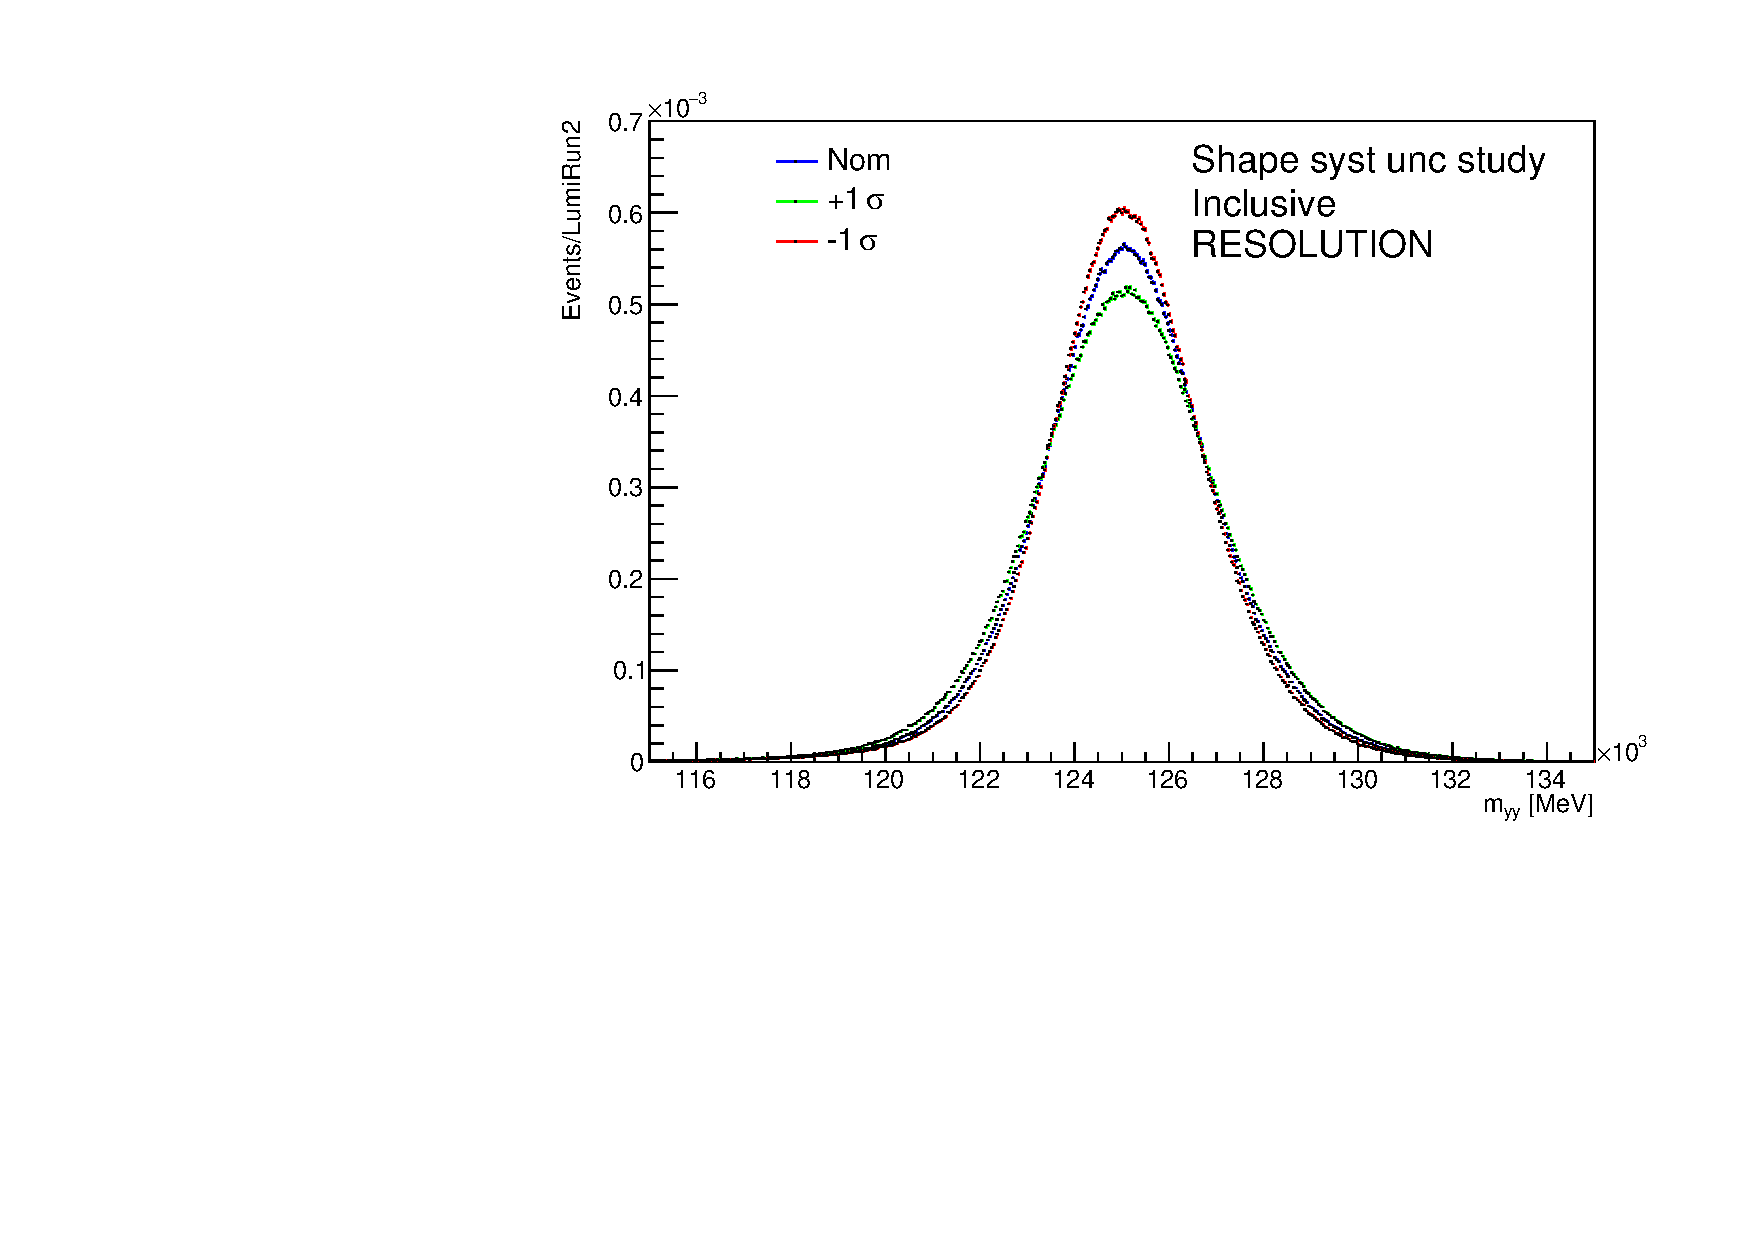
\includegraphics[width=.475\textwidth]{Pres_Images/HGam/Syst/var_shape_scale_no.pdf}
			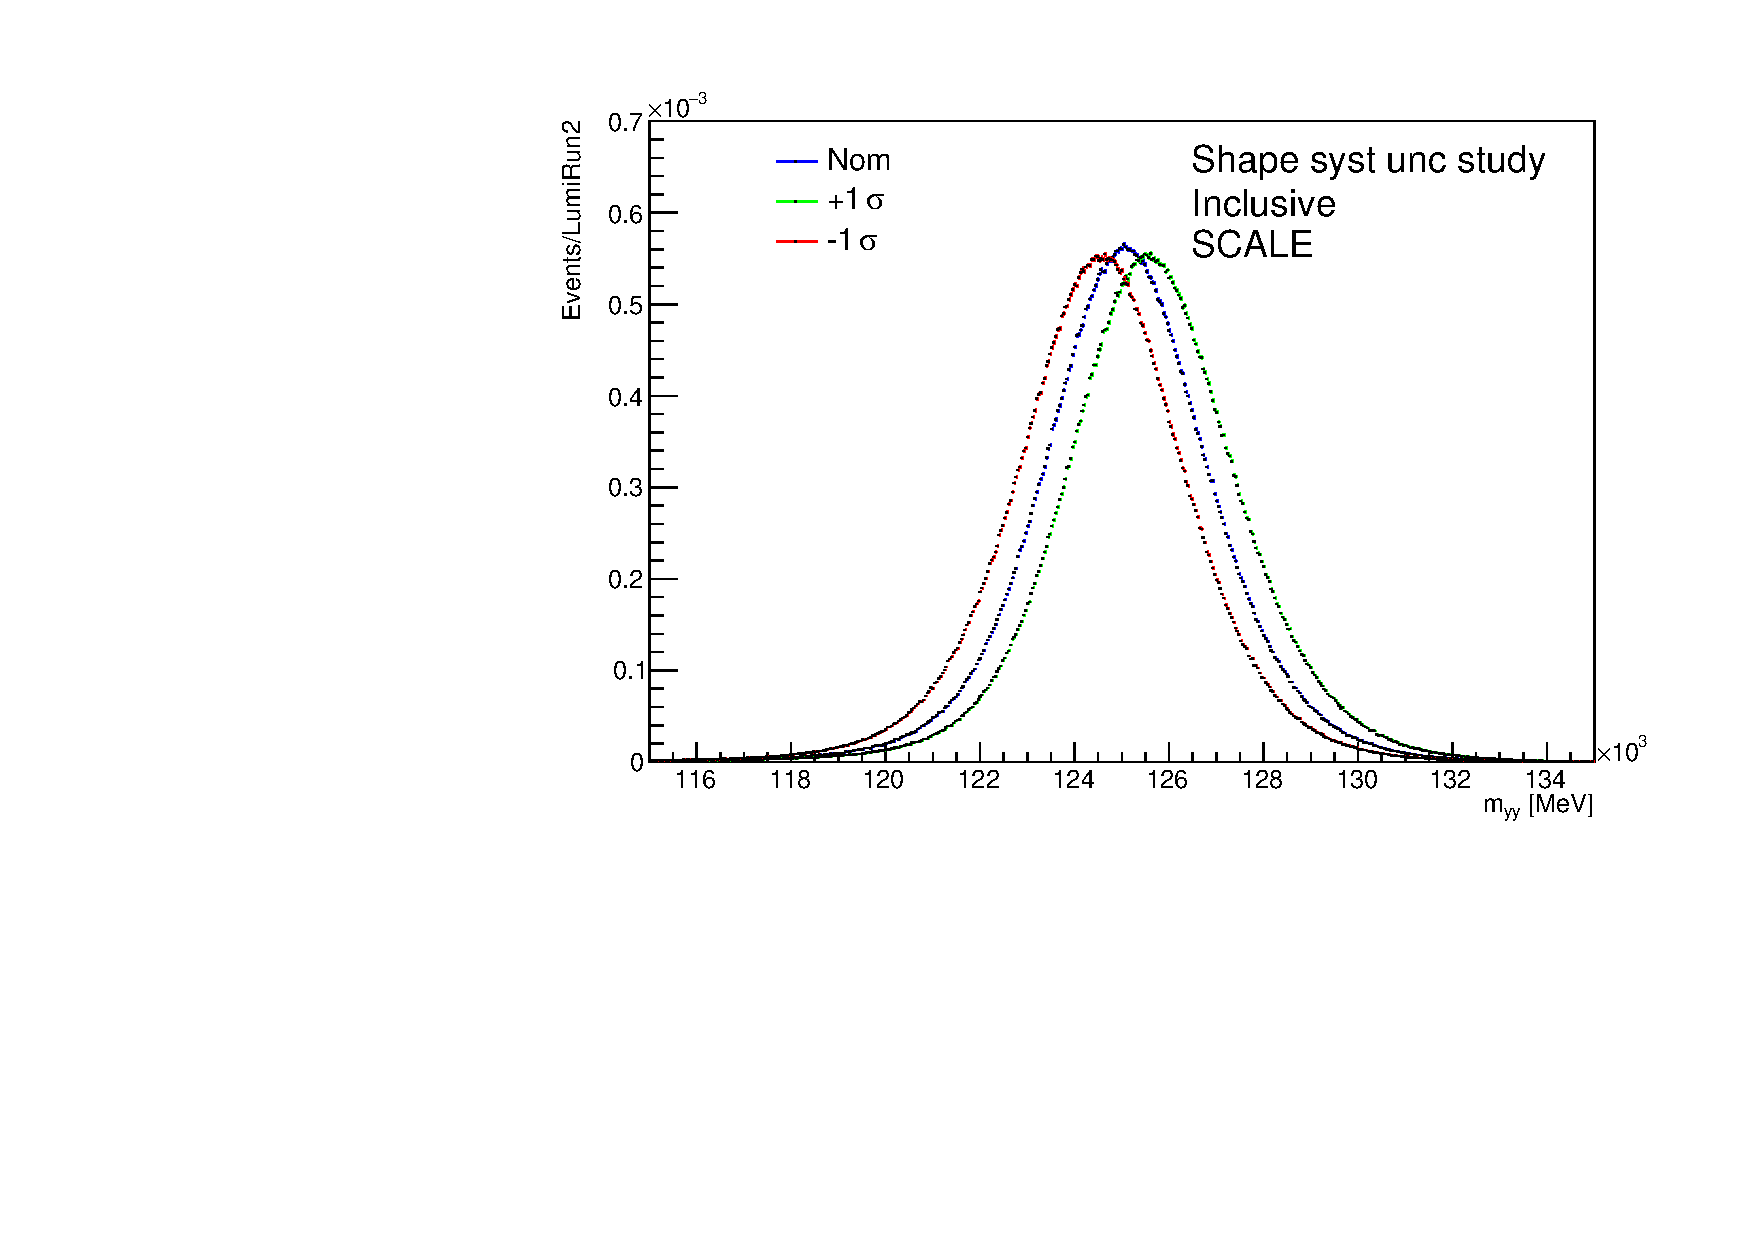
\includegraphics[width=.475\textwidth]{Pres_Images/HGam/Syst/var_shape_res_no.pdf}
		\end{center}
		\vfill
		
		\begin{textblock}{}(0.145,0.8)
			\small
			$\delta\sigma_c(\pm1\sigma)=\frac{IQR_c(\pm1\sigma)}{IQR_c}$
		\end{textblock}
		
		\begin{textblock}{}(0.595,0.8)
			\small
			$\delta\mu_c(\pm1\sigma)=\frac{<m_{\gamma\gamma}>_c(\pm1\sigma)}{<m_{\gamma\gamma}>_c}$
		\end{textblock}
	\end{frame}
	
	\begin{frame}{$\pm1\sigma$ var Shape uncertainties (ggF)}
		\vfill
		\centering
		\begin{table}[tbp]
			\centering
			\begin{tabular}{lcccc}
				\toprule[1.5pt]
				& \multicolumn{2}{c}{ATLAS\_EG\_RESOLUTION\_ALL}	
				& \multicolumn{2}{c}{ATLAS\_EG\_SCALE\_ALL}\\
				\midrule
				& \textbf{+1$\sigma$} & \textbf{-1$\sigma$}
				& \textbf{+1$\sigma$} & \textbf{-1$\sigma$}\\
				\cmidrule(lr){2-3} \cmidrule(lr){4-5}
				no& 0.0870621 & -0.0673568  & 0.00442256 & -0.00442571 \\
				1 & 0.0878635 & -0.0483741 	& 0.00261243 & -0.00261395 \\
				2 & 0.144179  & -0.0783765 	& 0.00319399 & -0.00318967 \\
				3 & 0.0847722 & -0.0719211  & 0.00489874 & -0.00490499 \\
				4 & 0.130348  & -0.106281   & 0.00581507 & -0.00581681 \\
				5 & 0.118665  & -0.116413   & 0.00935759 & -0.00937977 \\
				6 & 0.0728903 & -0.0417185  & 0.00280711 & -0.00280223 \\
				\bottomrule[1.5pt]
			\end{tabular}
			\caption{$\pm1\sigma$ var Resolution and Scale shape systematic uncertainties for each category}
		\end{table}
		\vfill
	\end{frame}
	
	\begin{frame}{Prod modes systematic uncertainty (ggF)}
		\vfill
		Production modes $C_X$ factors fitted using a linear fit($m_H$).
		\begin{center}
			\includegraphics[width=.8\textwidth]{Pres_Images/HGam/cx_all_prod_catConvEta_no.pdf}
			%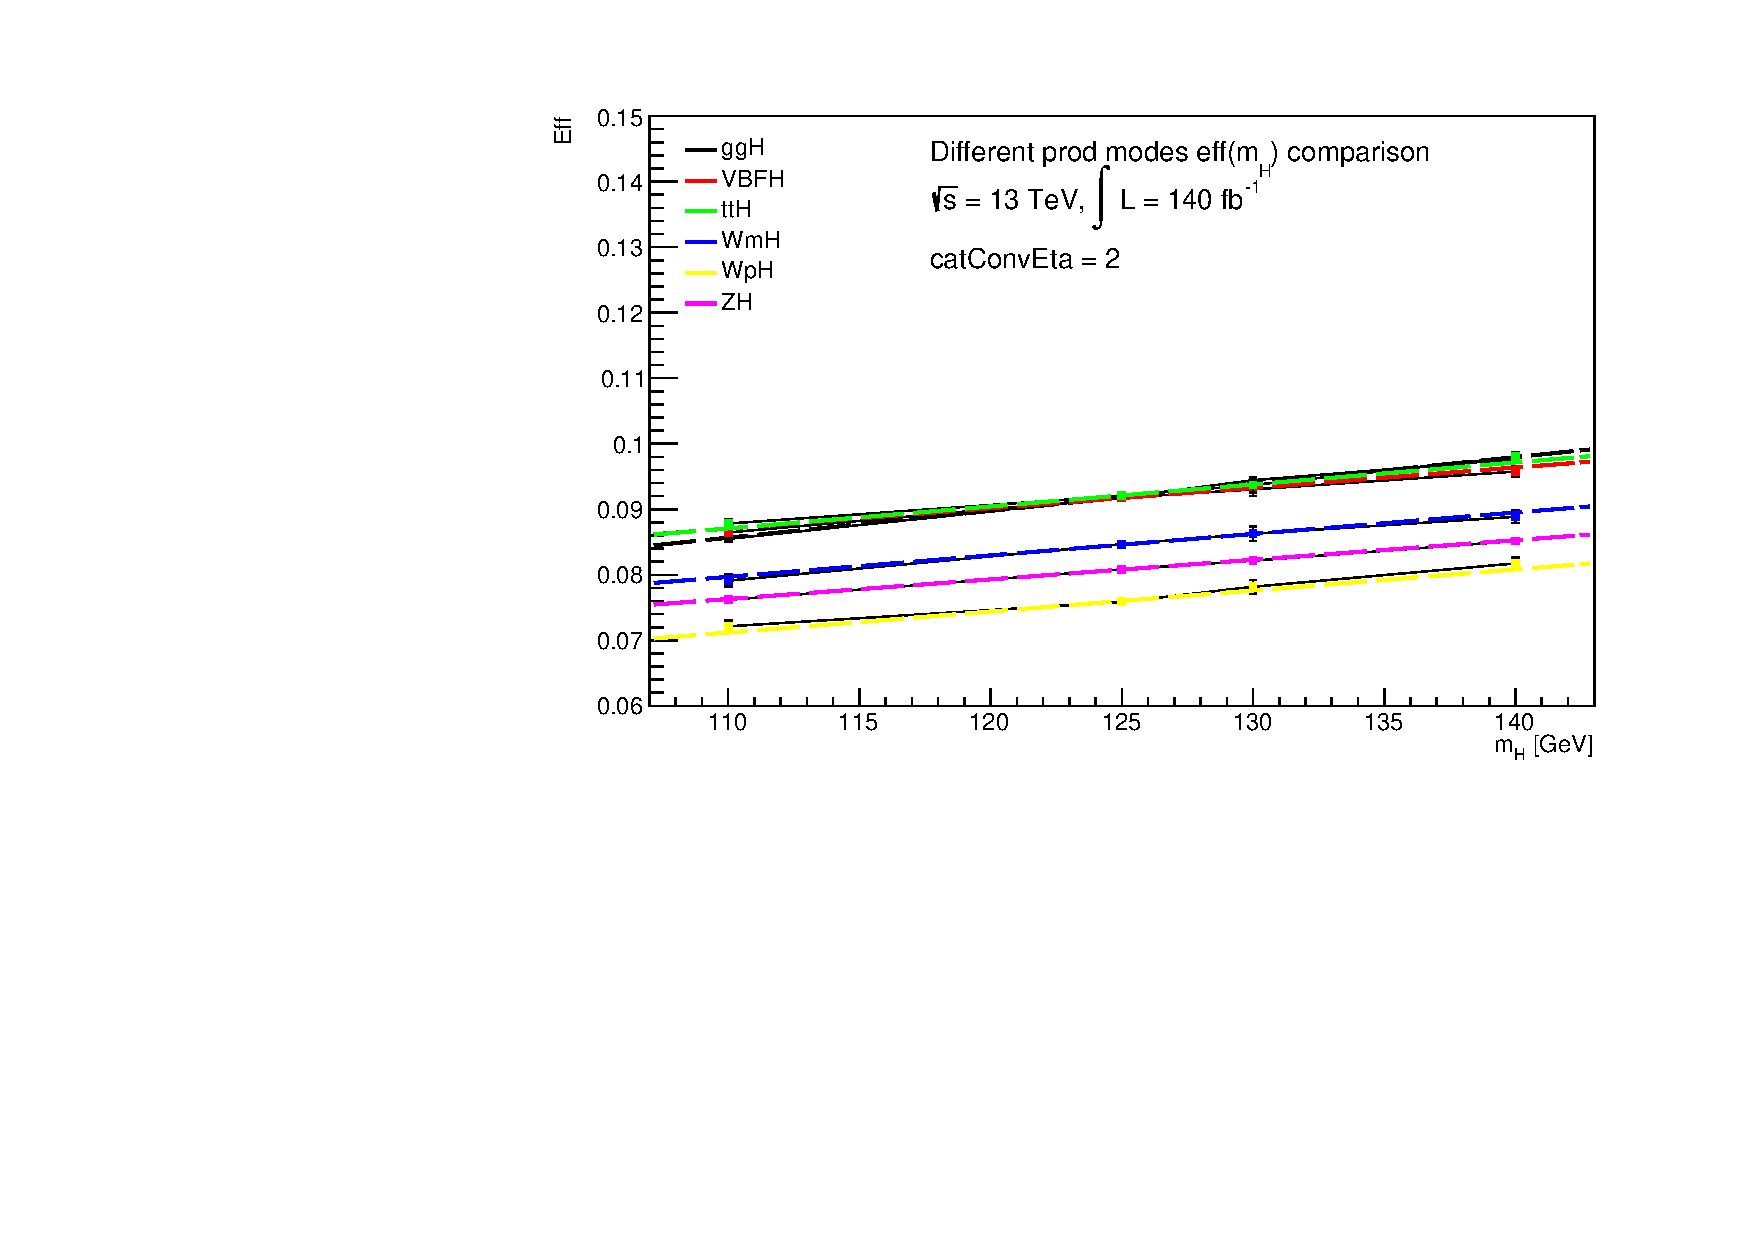
\includegraphics[width=.325\textwidth]{Pres_Images/Signal/eff_all_prod_cat_2.pdf}
			%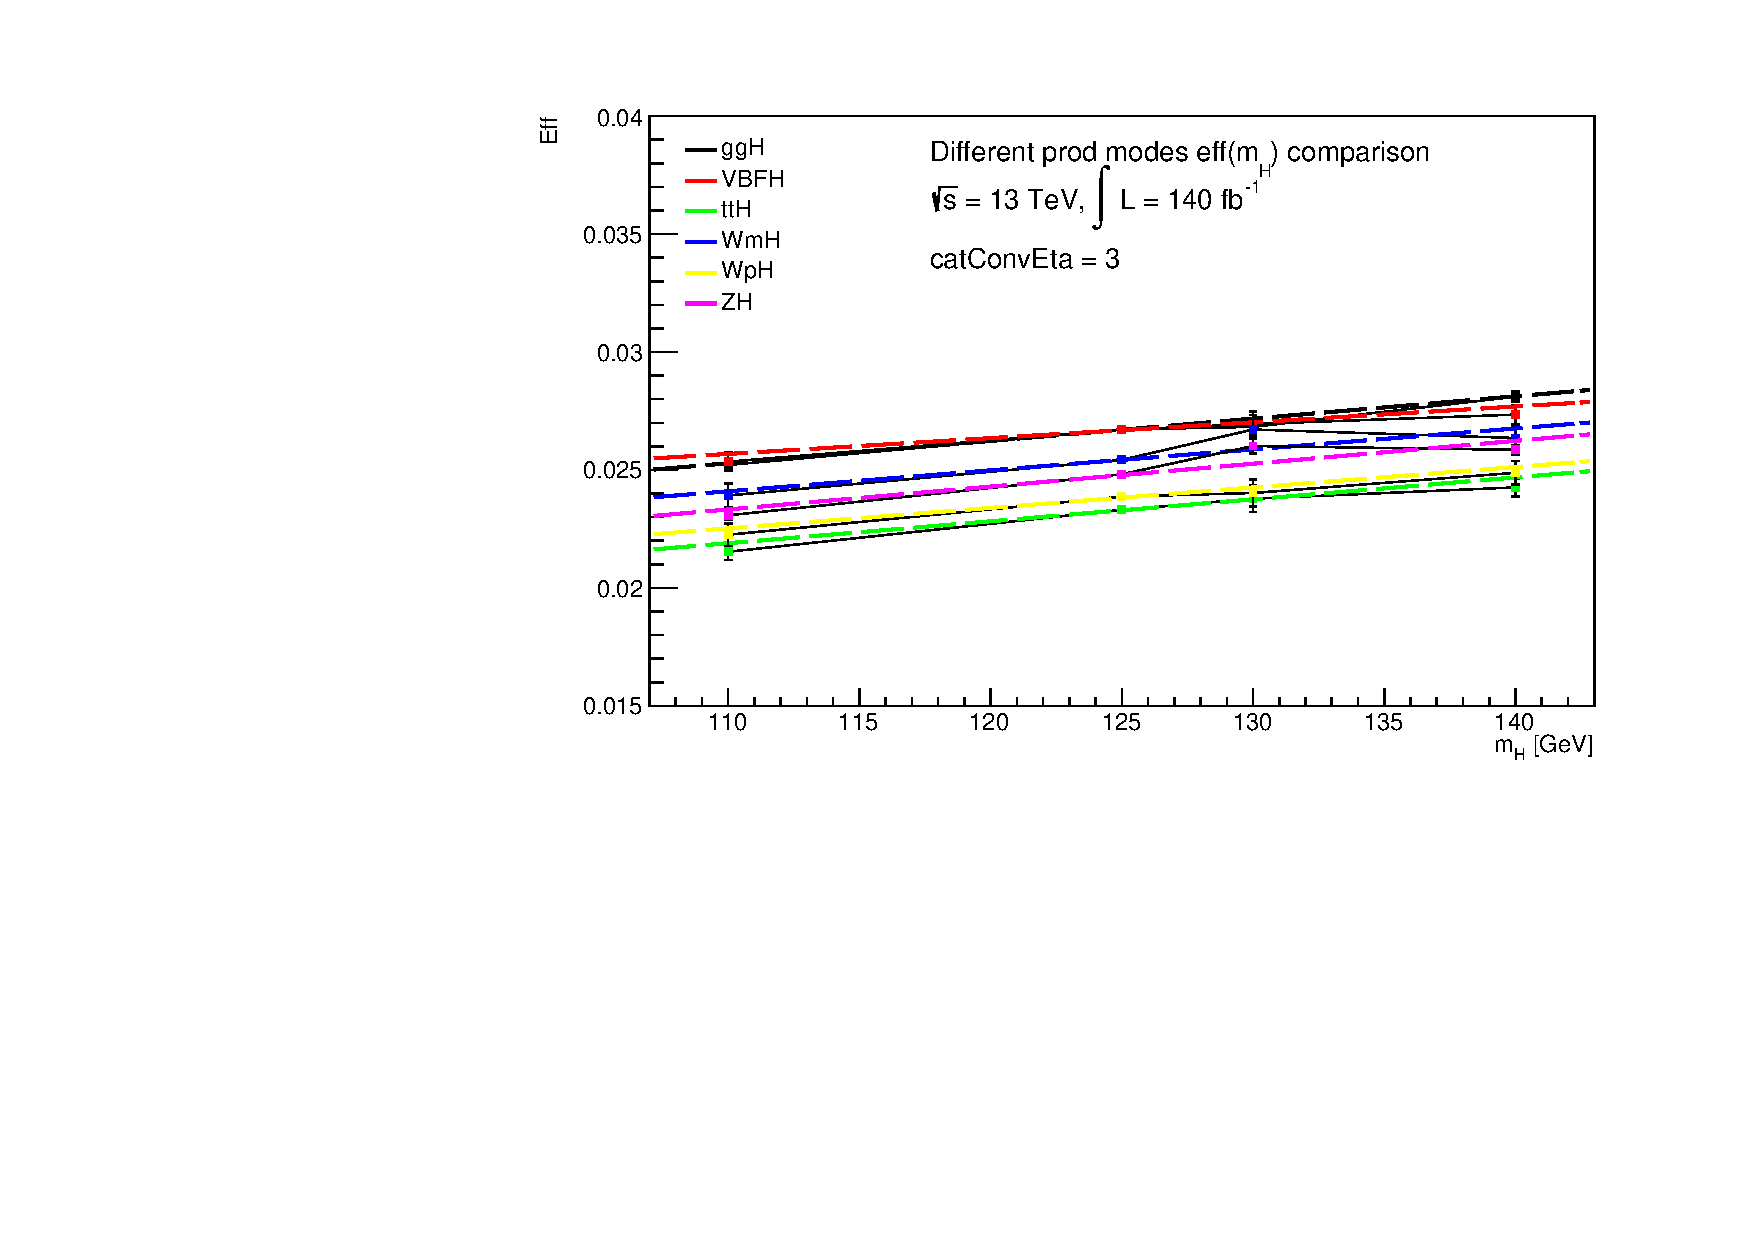
\includegraphics[width=.325\textwidth]{Pres_Images/Signal/eff_all_prod_cat_3.pdf}
			%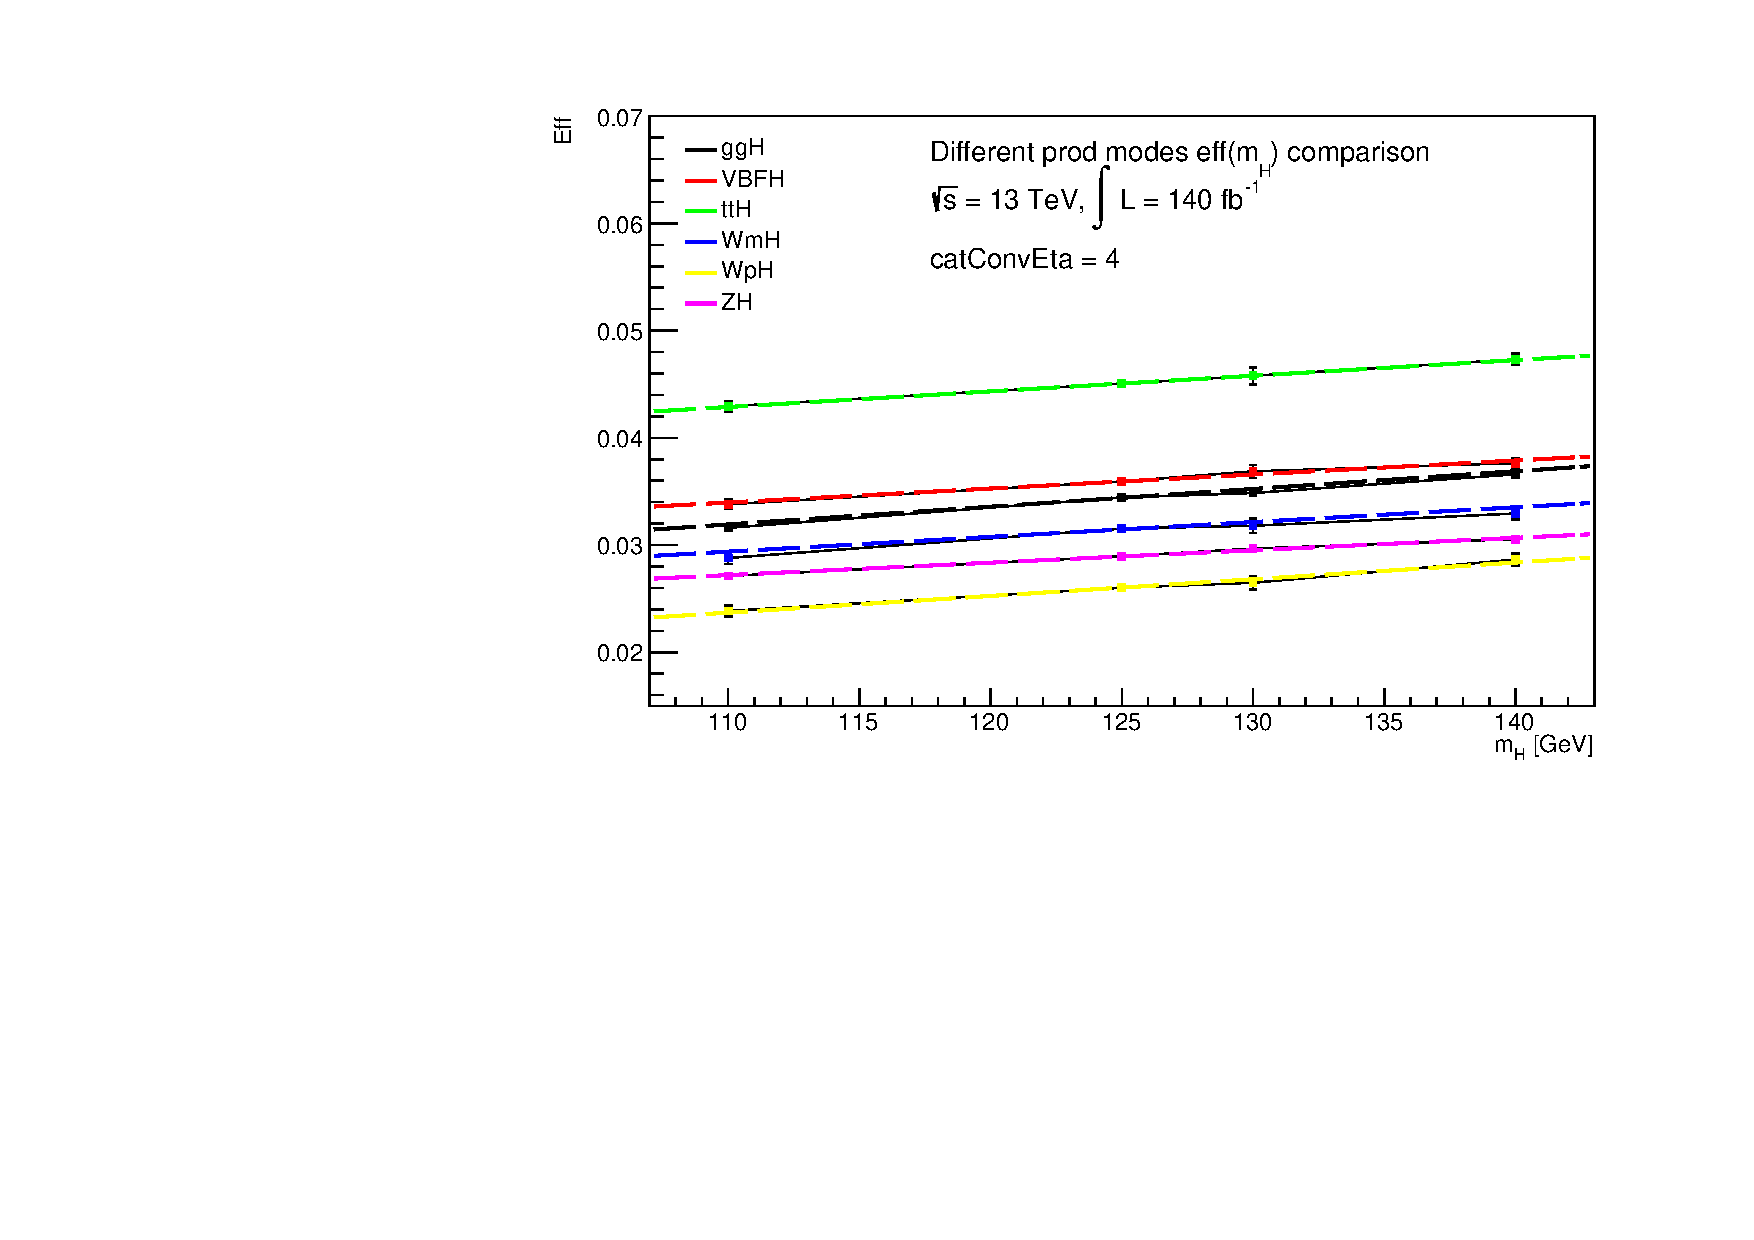
\includegraphics[width=.325\textwidth]{Pres_Images/Signal/eff_all_prod_cat_4.pdf}
			%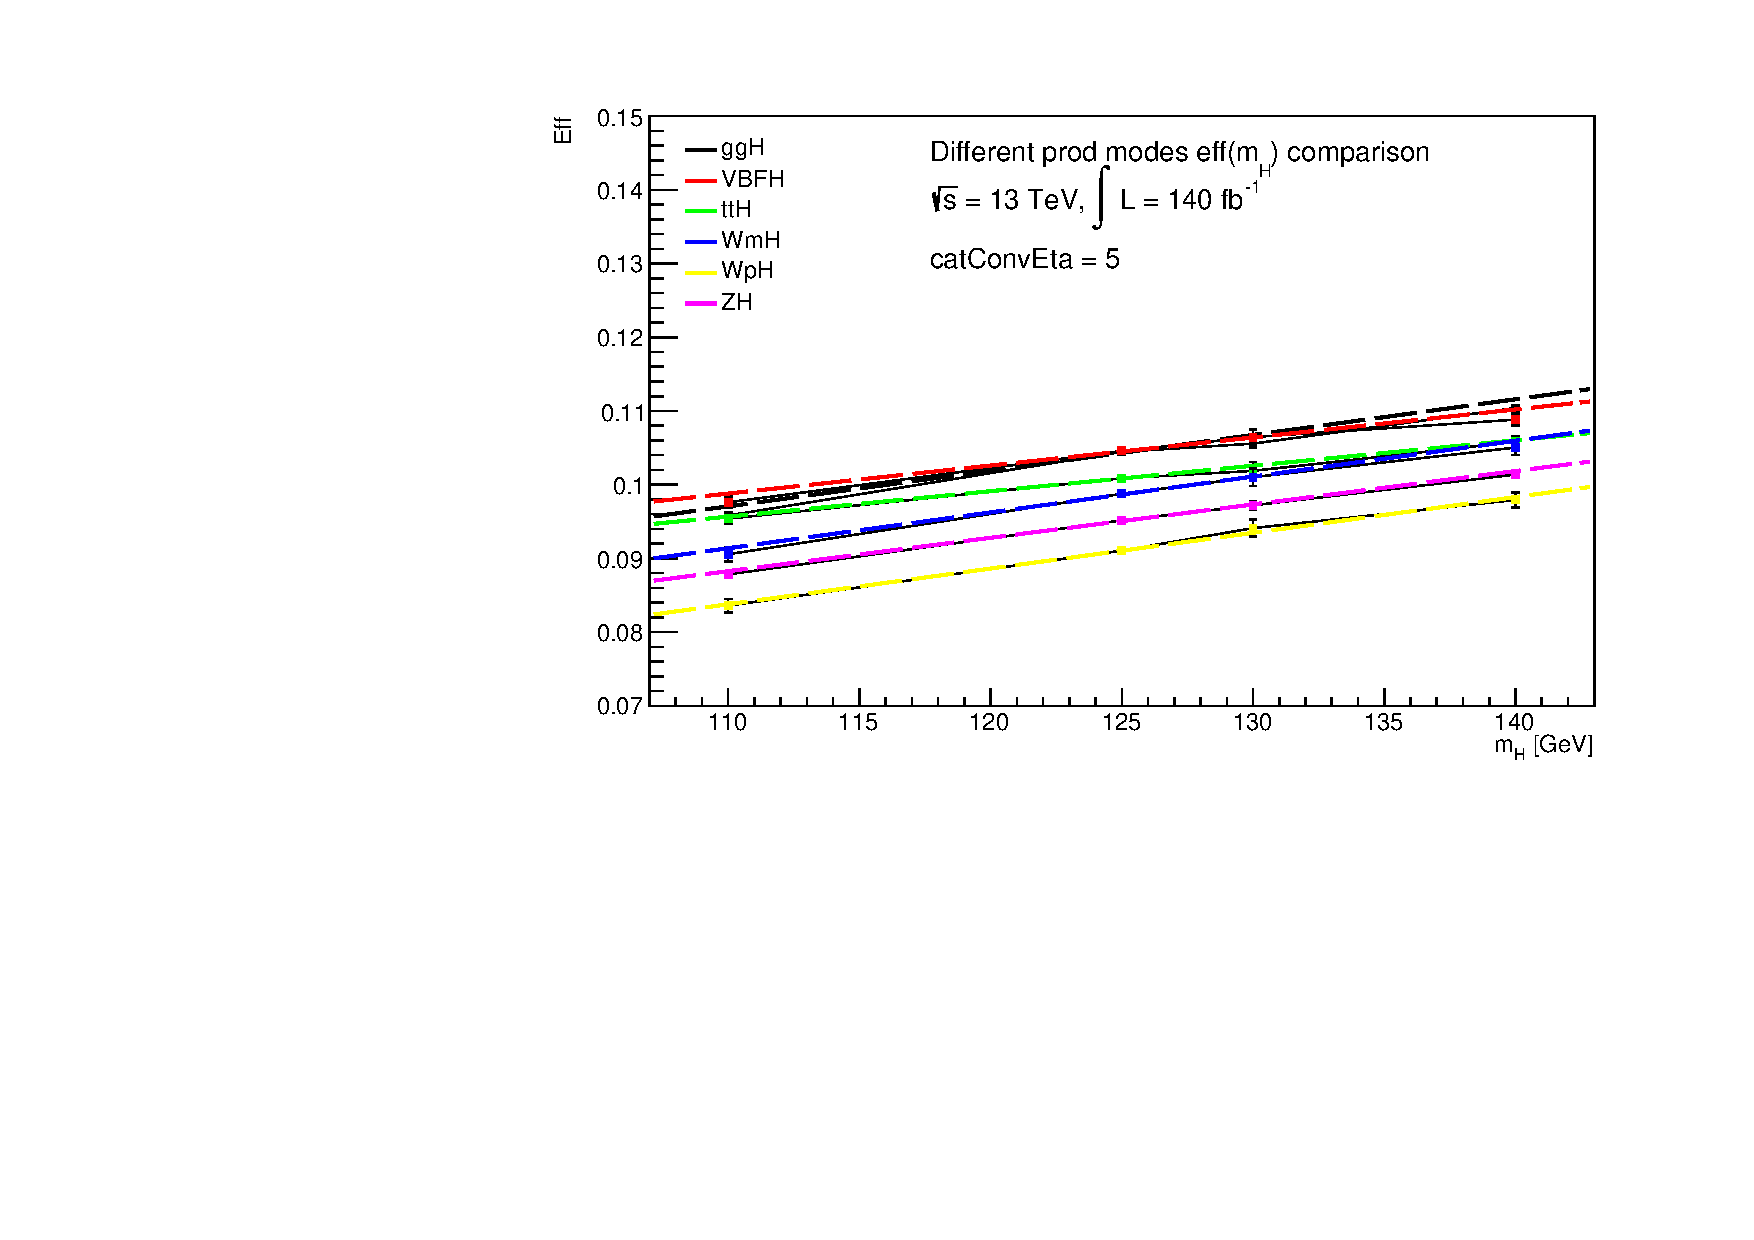
\includegraphics[width=.325\textwidth]{Pres_Images/Signal/eff_all_prod_cat_5.pdf}
			%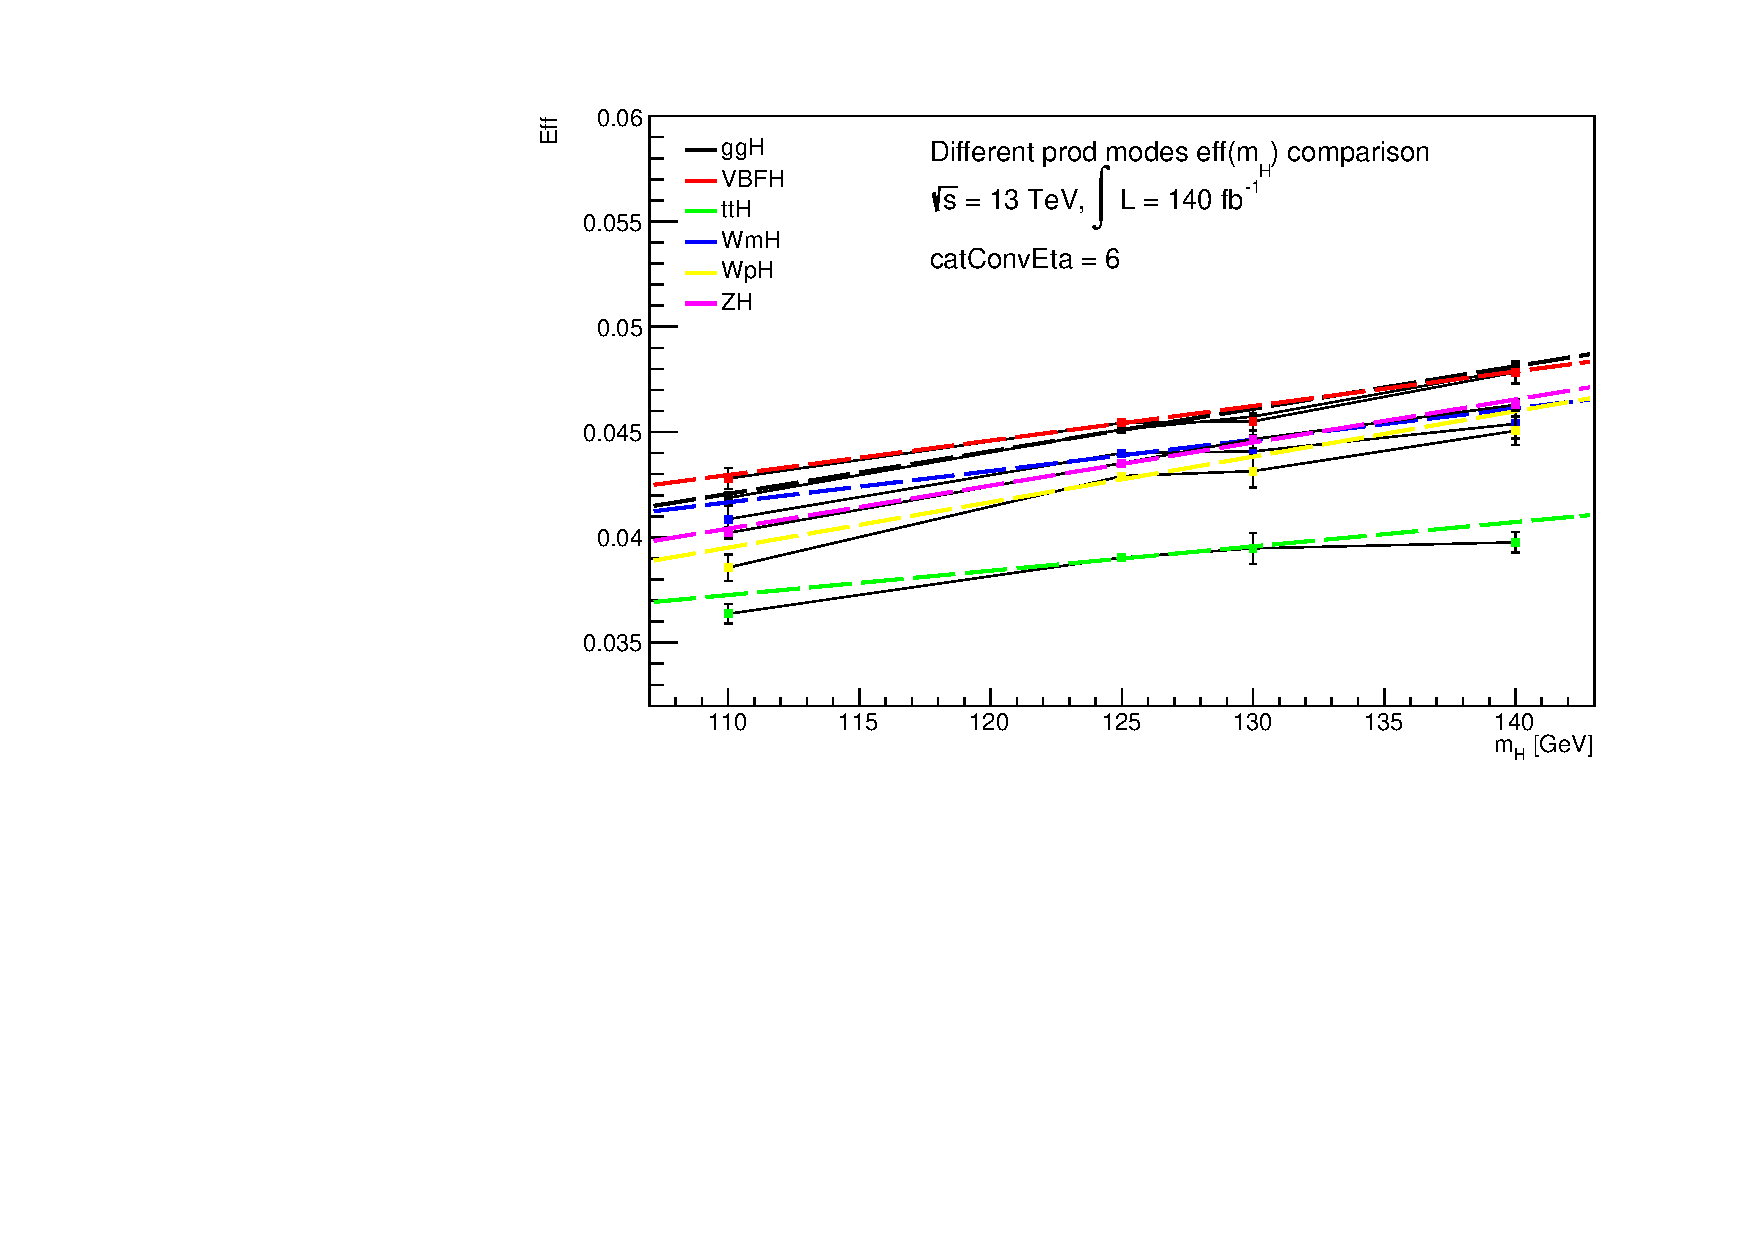
\includegraphics[width=.325\textwidth]{Pres_Images/Signal/eff_all_prod_cat_6.pdf}
		\end{center}
		\vfill
		\begin{textblock}{}(0.31,0.4)
			
\includegraphics[width=.2\textwidth]{Pres_Images/HGam/white.jpeg}
		\end{textblock}
		\begin{textblock}{}(0.36,0.405)
			\footnotesize
			Inclusive
		\end{textblock}
	\end{frame}

	
	\begin{frame}{Prod modes systematic uncertainty (ggF)}
		\vfill
		\begin{center}
			\includegraphics[width=.325\textwidth]{Pres_Images/HGam/cx_all_prod_catConvEta_1.pdf}
			\includegraphics[width=.325\textwidth]{Pres_Images/HGam/cx_all_prod_catConvEta_2.pdf}
			\includegraphics[width=.325\textwidth]{Pres_Images/HGam/cx_all_prod_catConvEta_3.pdf}
			\includegraphics[width=.325\textwidth]{Pres_Images/HGam/cx_all_prod_catConvEta_4.pdf}
			\includegraphics[width=.325\textwidth]{Pres_Images/HGam/cx_all_prod_catConvEta_5.pdf}
			\includegraphics[width=.325\textwidth]{Pres_Images/HGam/cx_all_prod_catConvEta_6.pdf}
			%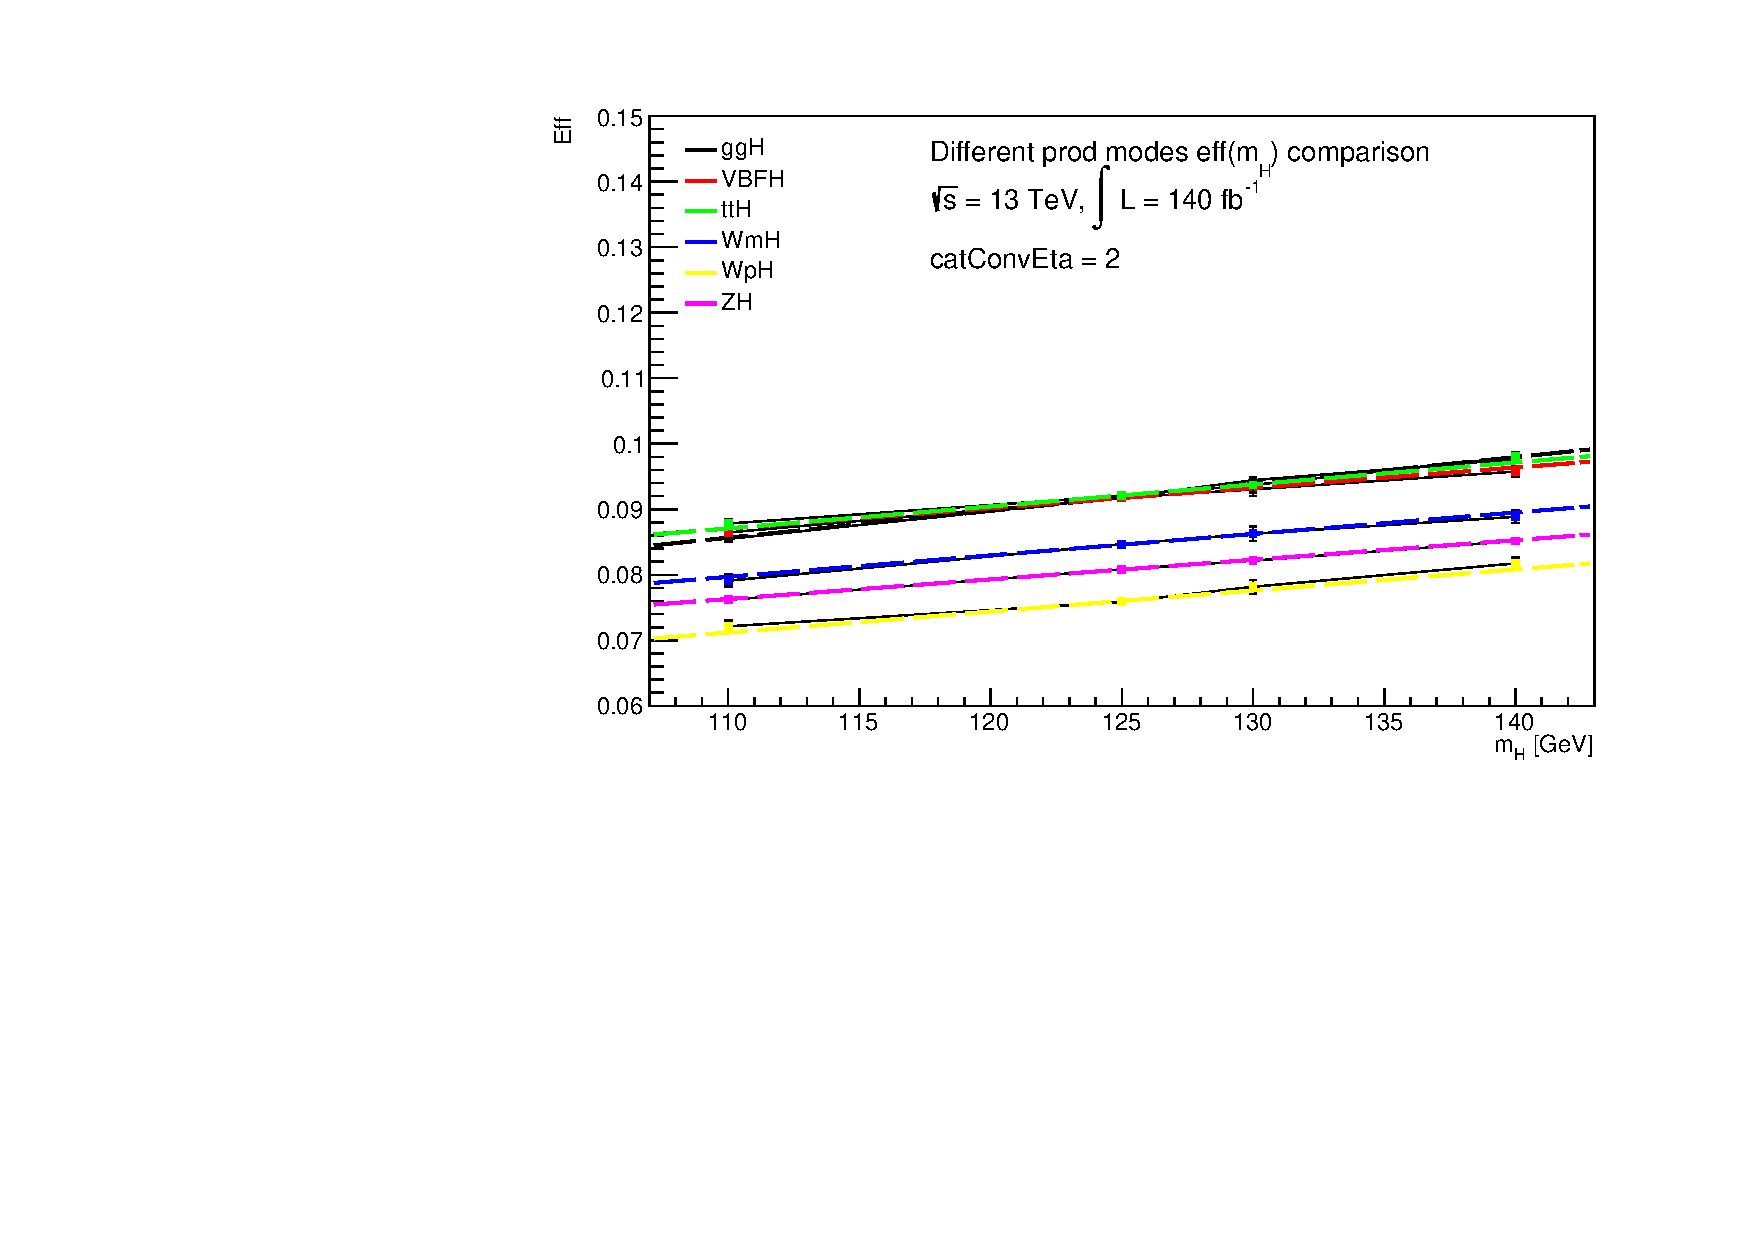
\includegraphics[width=.325\textwidth]{Pres_Images/Signal/eff_all_prod_cat_2.pdf}
			%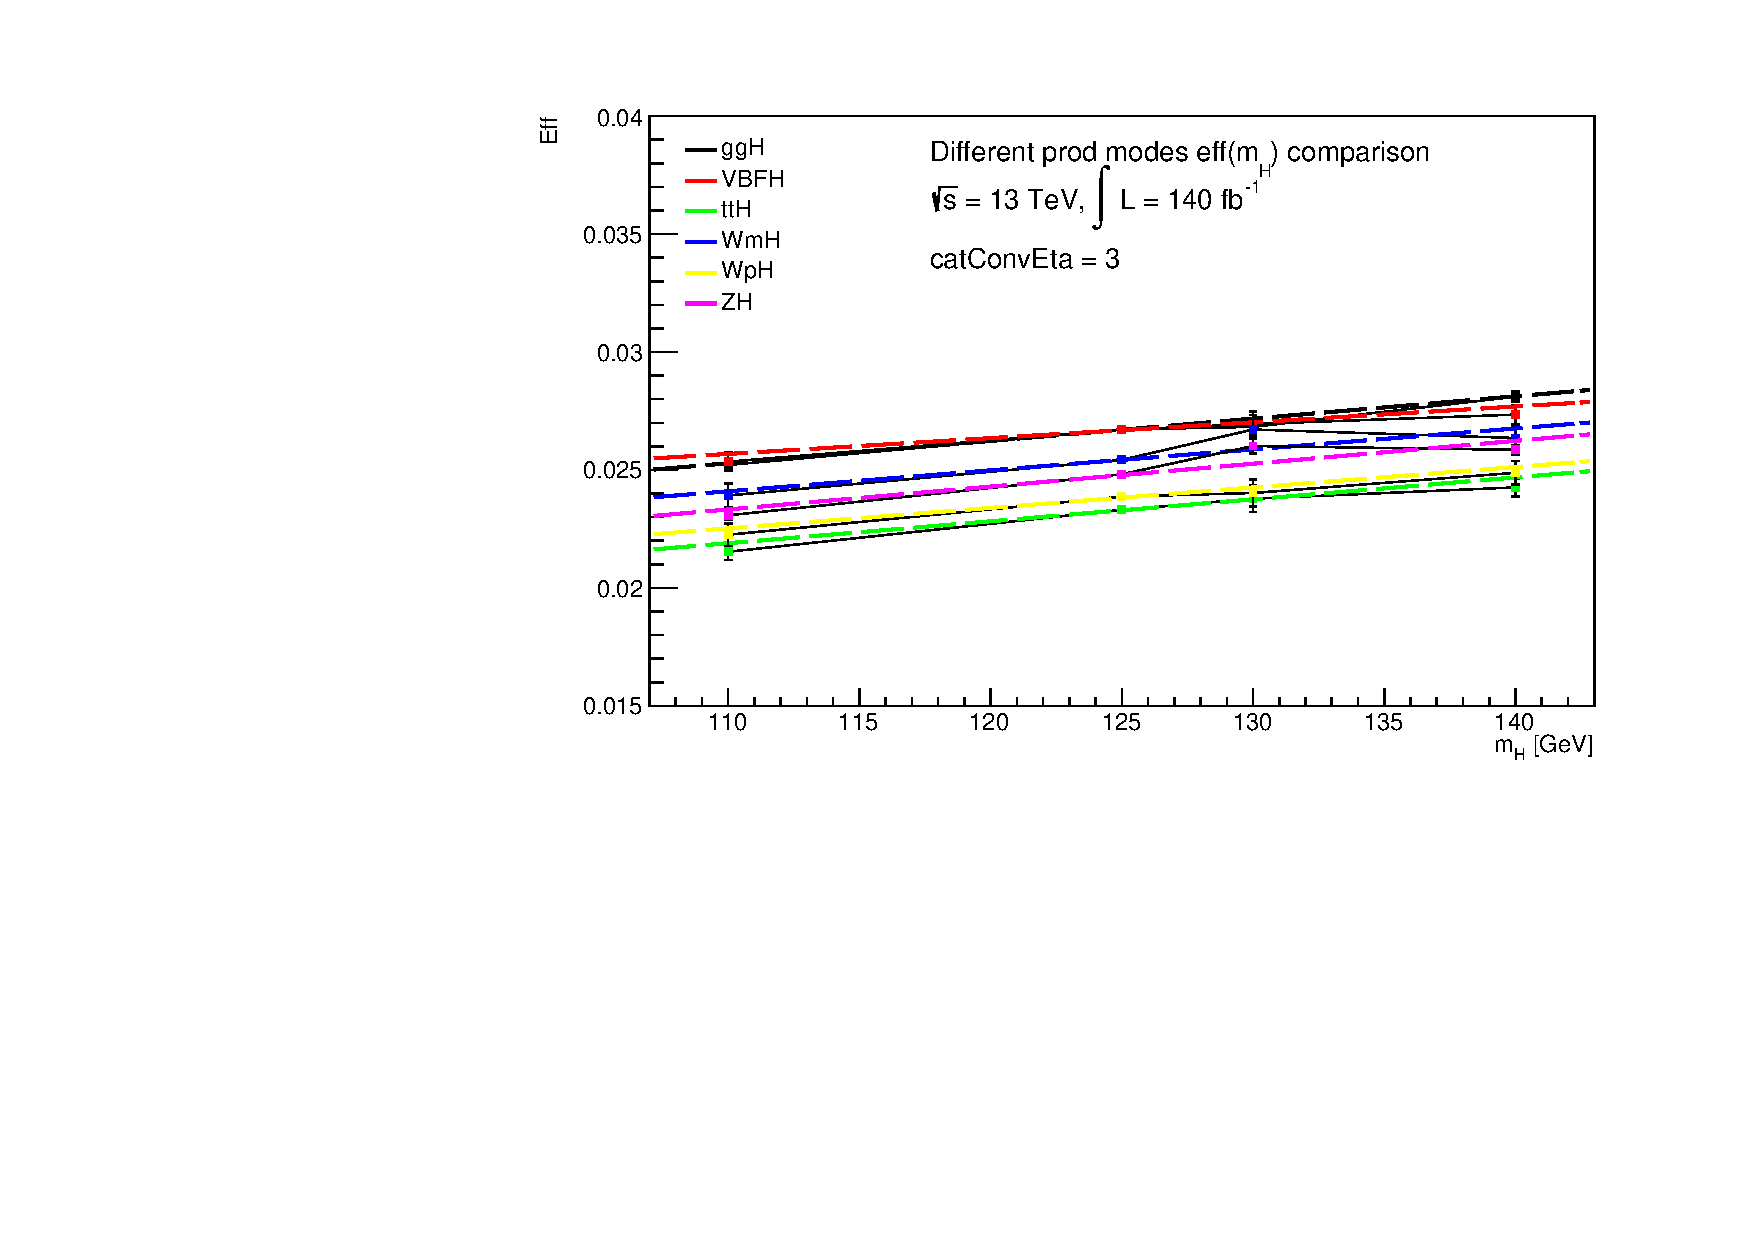
\includegraphics[width=.325\textwidth]{Pres_Images/Signal/eff_all_prod_cat_3.pdf}
			%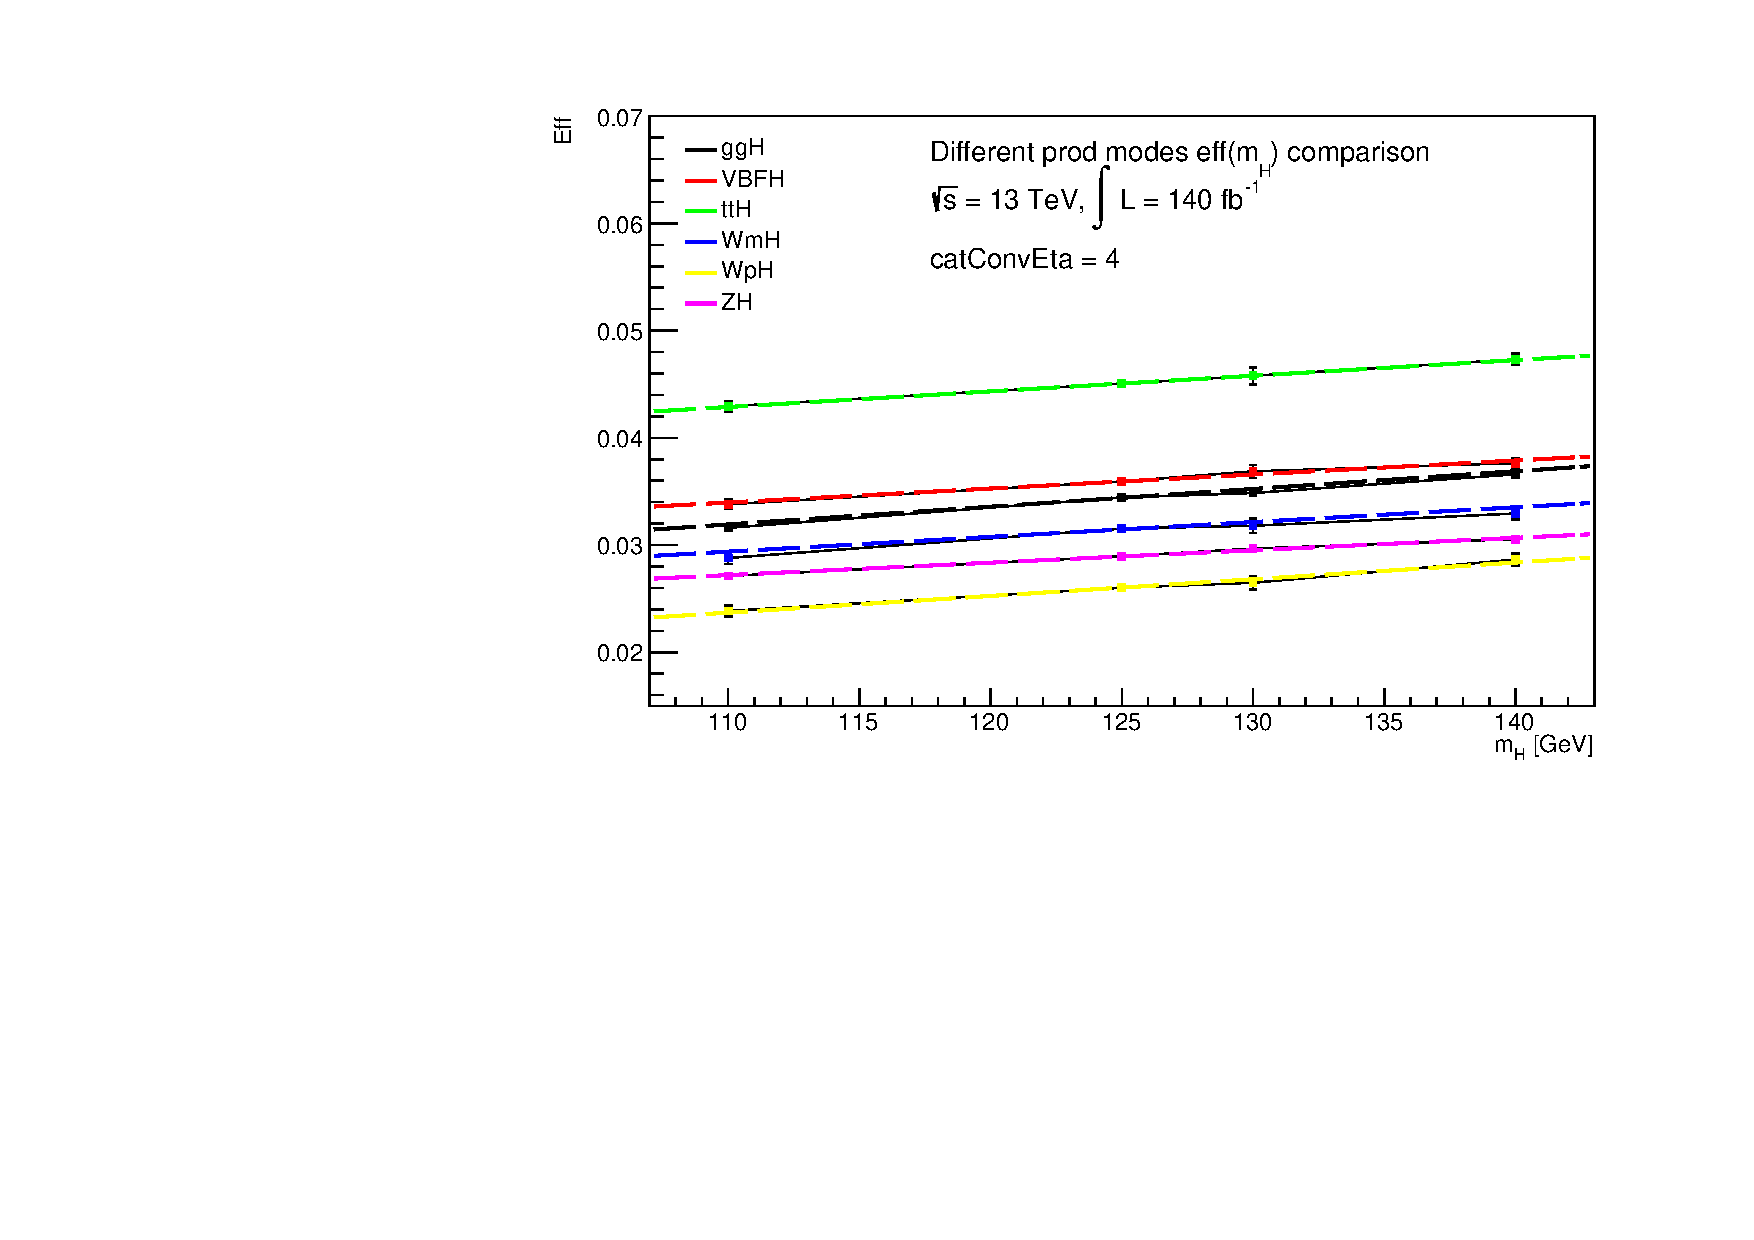
\includegraphics[width=.325\textwidth]{Pres_Images/Signal/eff_all_prod_cat_4.pdf}
			%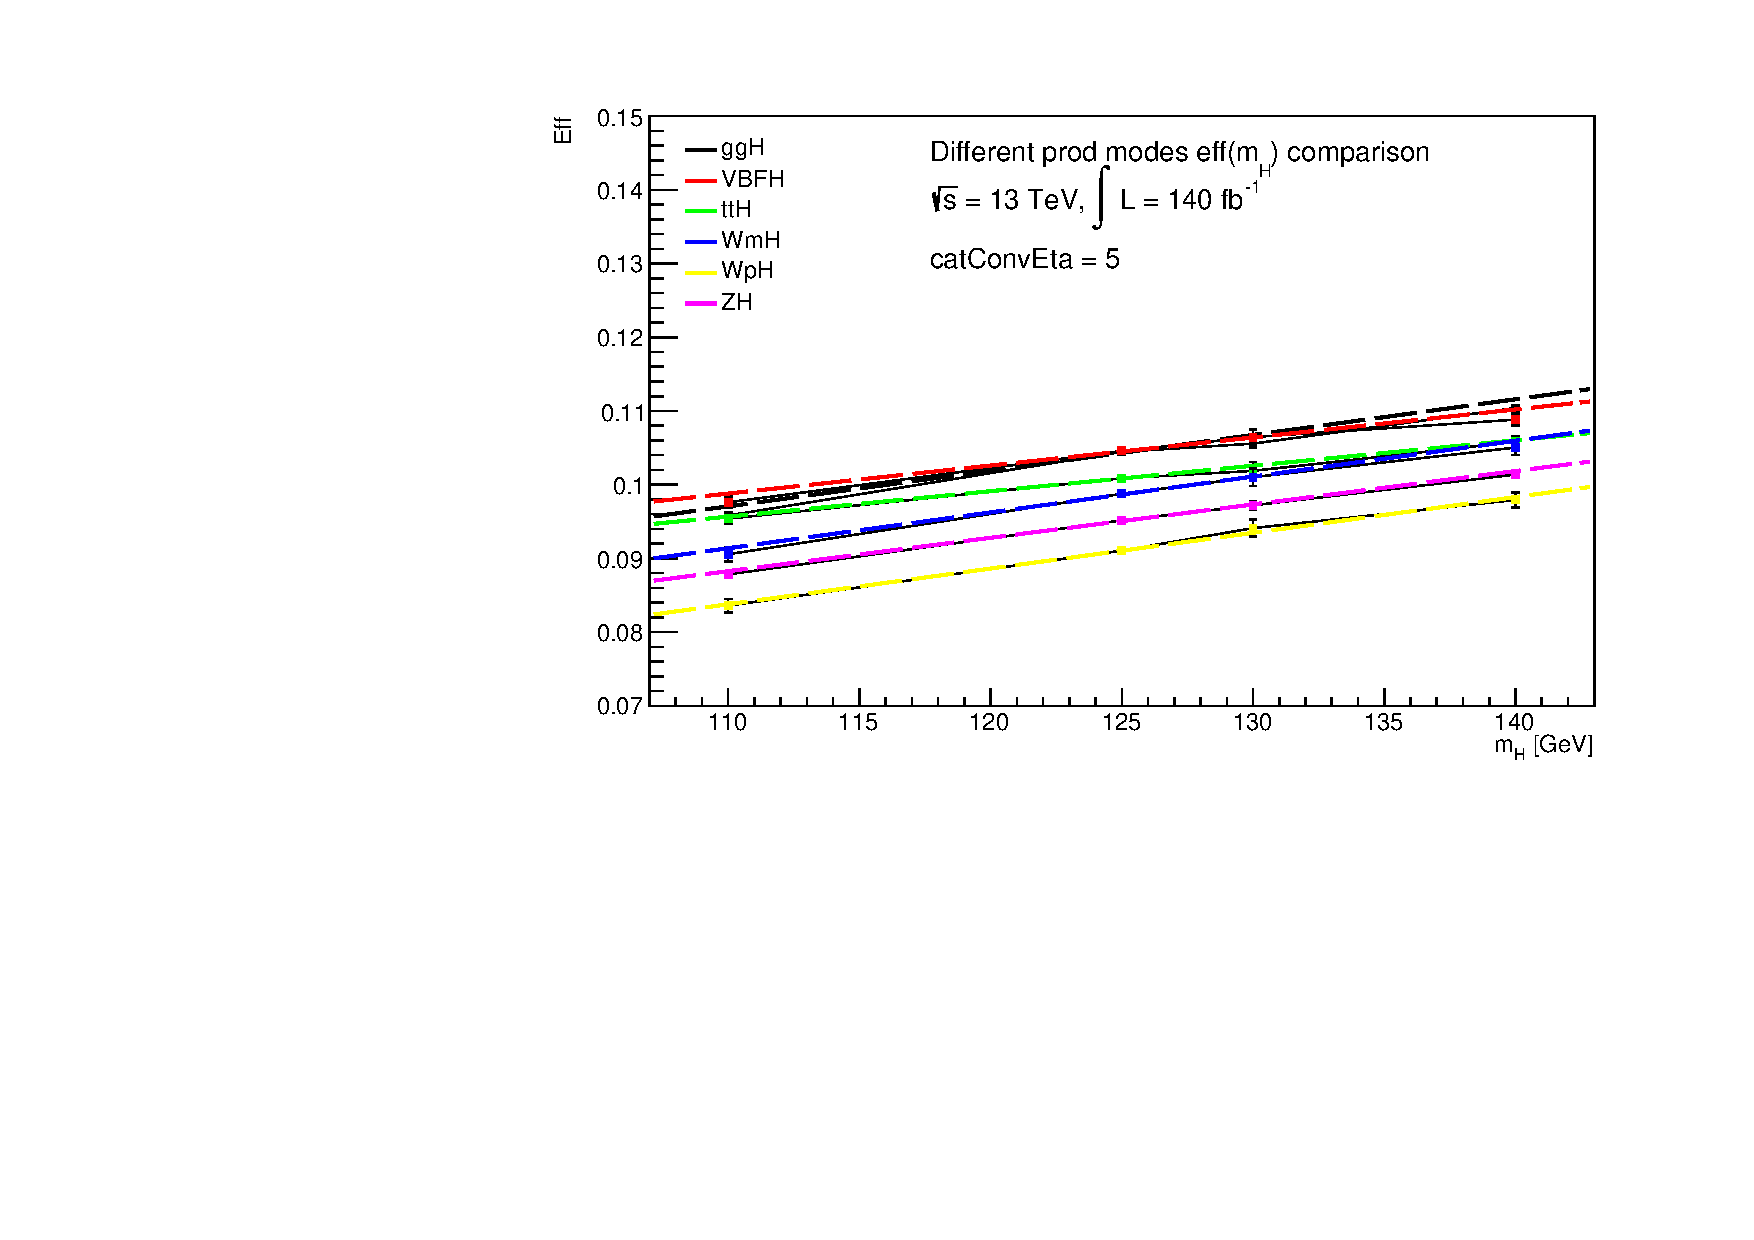
\includegraphics[width=.325\textwidth]{Pres_Images/Signal/eff_all_prod_cat_5.pdf}
			%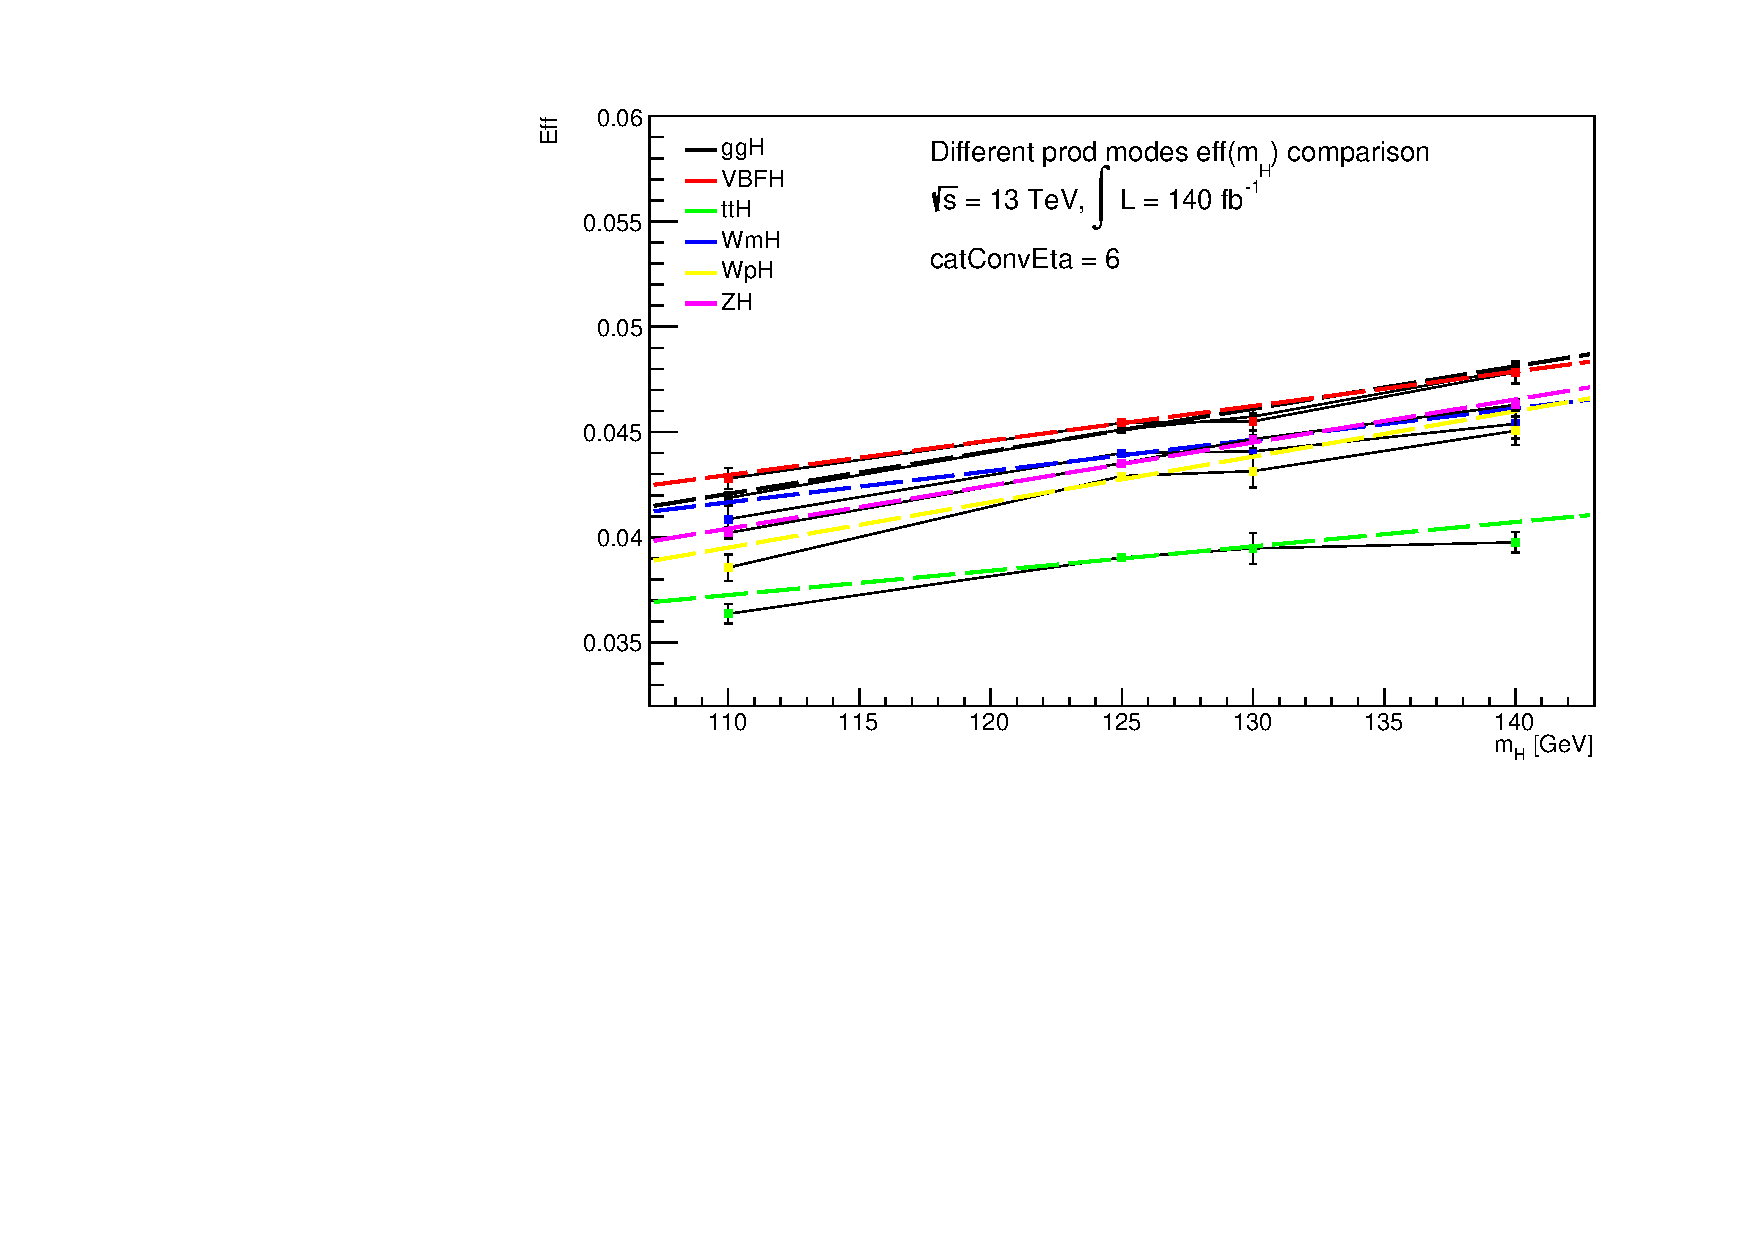
\includegraphics[width=.325\textwidth]{Pres_Images/Signal/eff_all_prod_cat_6.pdf}
		\end{center}
	\end{frame}
	
	\begin{frame}{Prod modes systematic uncertainty (ggF)}
		\vfill
		The other production mode systematic uncertainty for each category is the maximum of  $$\dfrac{|C^{fit}_{X\ prod}-C^{fit}_{X\ ggF}|}{C^{fit}_{X\ ggF}}$$ by varying prod modes and resonance mass (110,125,130,140 GeV)
		
		\begin{itemize}
			\item Inclusive		 $\to \sigma=$ 0.0439428
			\item \texttt{catConvEta} = 1 $\to \sigma=$ 0.260816
			\item \texttt{catConvEta} = 2 $\to \sigma=$ 0.069153
			\item \texttt{catConvEta} = 3 $\to \sigma=$ 0.176629
			\item \texttt{catConvEta} = 4 $\to \sigma=$ 0.274333
			\item \texttt{catConvEta} = 5 $\to \sigma=$ 0.108577
			\item \texttt{catConvEta} = 6 $\to \sigma=$ 0.207507
		\end{itemize}
		\vfill
	\end{frame}

	\begin{frame}{HSM systematic uncertainties}
		\vfill
		The Higgs Standard Model background (HSM) systematic uncertainties are:
		\begin{itemize}
			\item yield and shape systematic uncertainties $\to$ estimated as the signal but using the merged distribution and without \texttt{isFiducialLowMyy} selections ($C_X \to$ eff)
			\item no production modes systematic uncertainty
			\item the SM Higgs mass uncertainty (0.19\%) is also included.
		\end{itemize}
		\vfill
	\end{frame}

	\begin{frame}{Asimov Data}
		\vfill
		In order to test the model three Asimov dataset have been created:
		\begin{center}
			\begin{table}[tbp]
				\centering
				\begin{tabular}{lccccc}
					\toprule[1.pt]
											& Non-res bkg	& HSM bkg		& sig			& $\mu$	& $m_H$		\\
					\midrule
					AsimovData\_1\_mH125	& \checkmark	& \checkmark	& \checkmark	& 1		& 125.09 GeV	\\
					AsimovData\_1\_mH140	& \checkmark	& \checkmark	& \checkmark	& 1		& 140 GeV		\\
					AsimovData\_0			& \checkmark	& \checkmark	& X				& 0		& //		\\
					\bottomrule[1.pt]
				\end{tabular}
			\end{table}
		
		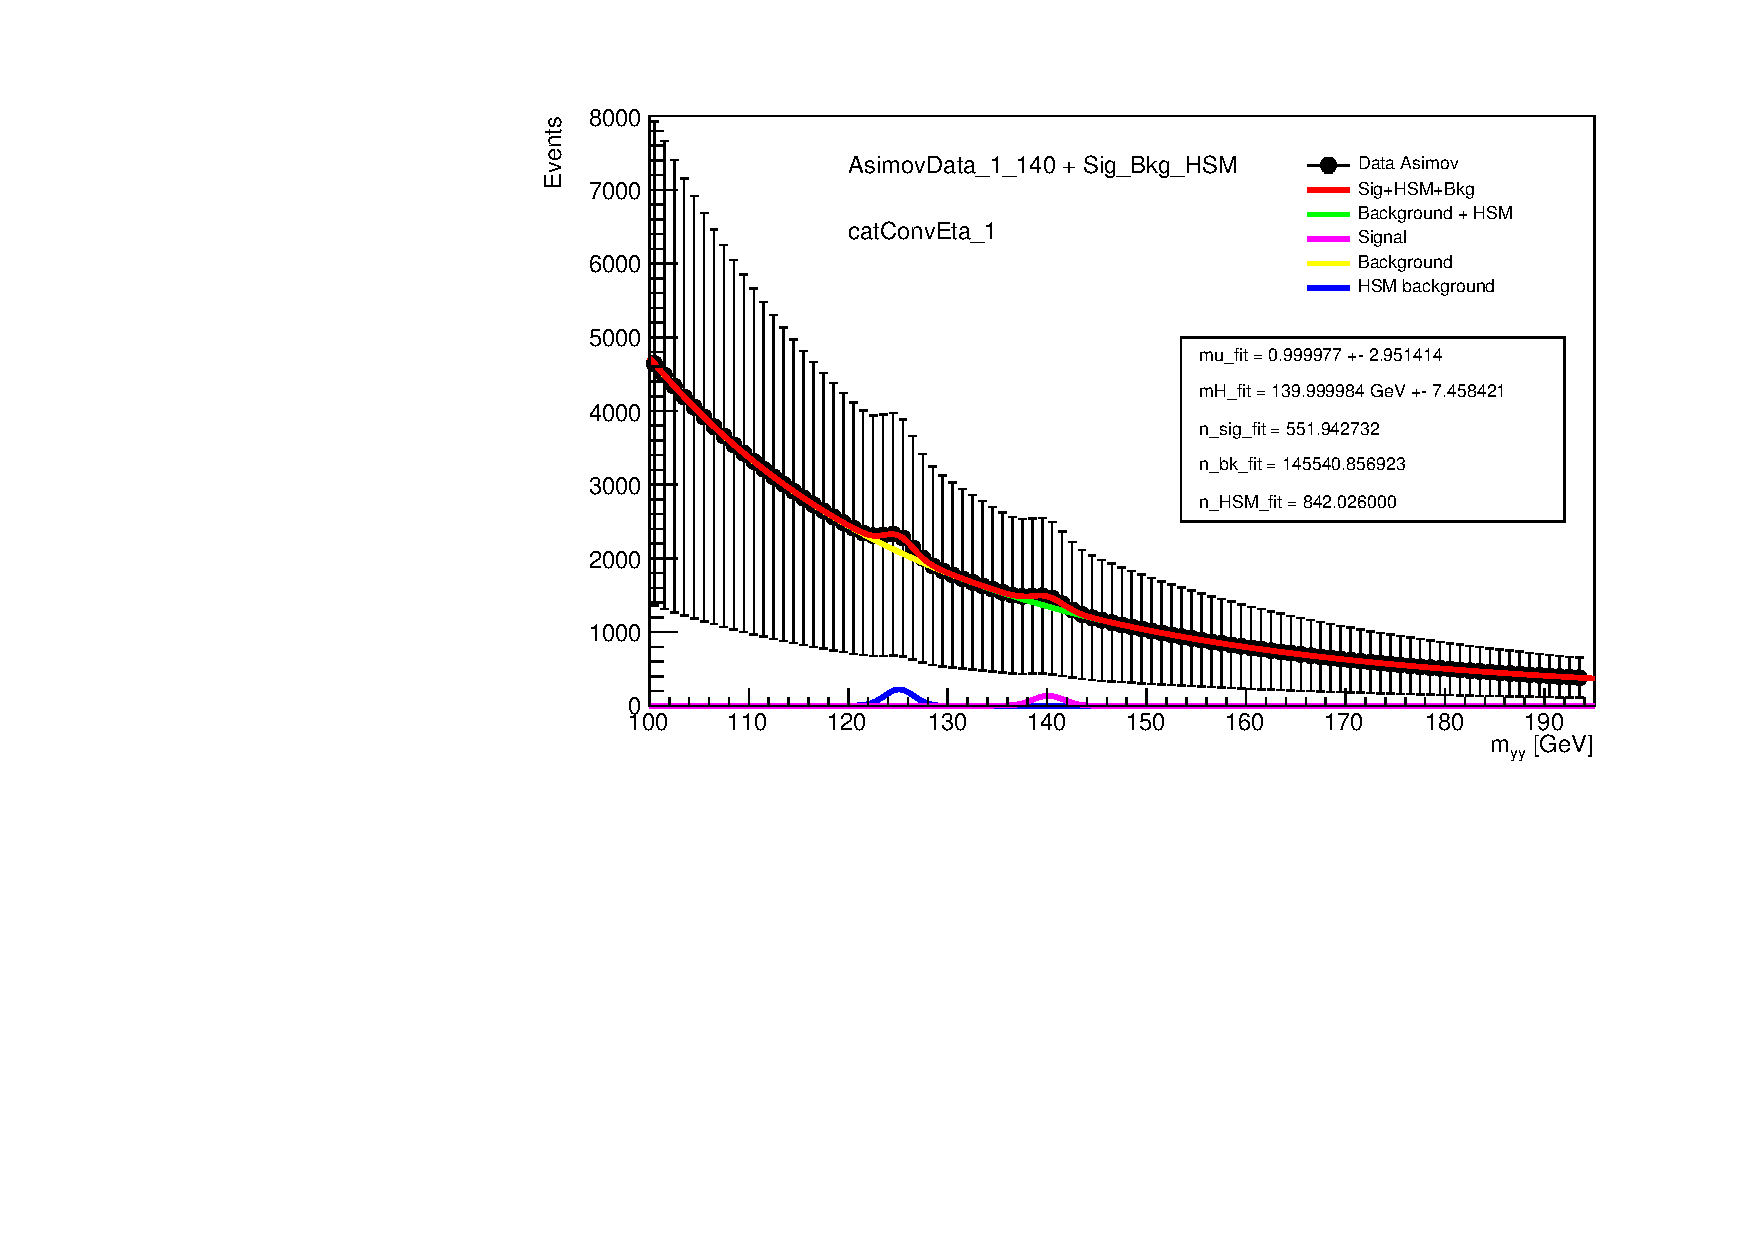
\includegraphics[width=.7\textwidth]{Pres_Images/HGam/HSM_AsimovData_1_140_catConvEta_1.pdf}
		\end{center}
		%\begin{textblock}{}(0.625,0.5)
		%	\small
		%	\begin{itemize}
		%		\item $\mu = 1$;
		%		\item $m_H = 125.09$ GeV;
		%		\item $\mu^{fit} = 0.994 \pm 0.097$;
		%		\item $m^{fit}_H = 125.109 \pm 0.229$ GeV;
		%	\end{itemize}
		%\end{textblock}
		\vfill
	\end{frame}
	
	%%%%%%%%% Results %%%%%%%%%
	\section{Expected Results}
	\SectionPage
	
	\begin{frame}{Limits}
		\vfill
		\begin{center}
			\includegraphics[width=1.\textwidth]{Pres_Images/HGam/plot_AsimovData_0_ggHyy_MC_catConvEta_syst_HSM_fid.pdf}\\
		\end{center}
		\vfill
	\end{frame}
	
	%\begin{frame}{Systematic analysis impact}
	%	\vfill
	%	\begin{center}
	%		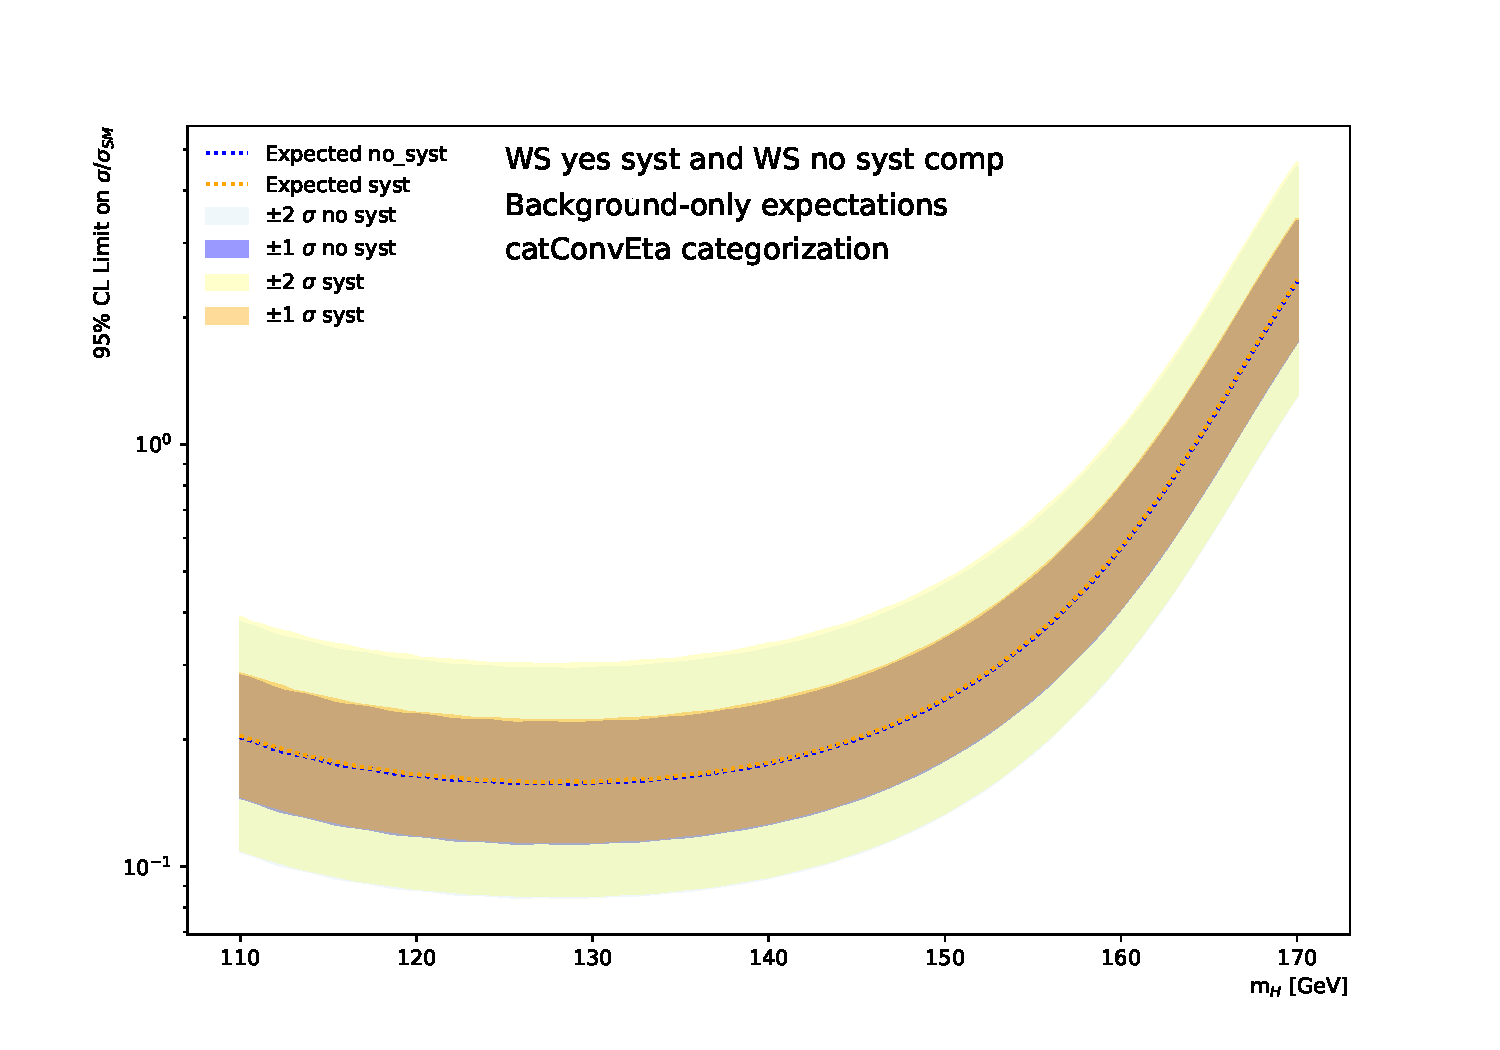
\includegraphics[width=1.\textwidth]{Pres_Images/HGam/plot_syst.pdf}\\
	%	\end{center}
	%	\vfill
	%\end{frame}
	
	\begin{frame}{p0 Scan}
		\centering
		\includegraphics[width=.9\textwidth]{Pres_Images/HGam/p0_catConvEta_syst_HSM_fid.pdf}
	\end{frame}
	
	\begin{frame}{Conclusions}
		\vfill
		\begin{itemize}
			\item Almost all analysis building blocks ready:
			\begin{itemize}
				\item the signal model as a function of the $m_H$ works;
				\item baseline categorisation to avoid prod-mode dependence provides a small improvement;
				\item the backgrounds (non-res + HSM) are included;
				\item using fiducial events showed a reduction in model dependence.
				\item the expected $p_0$ and limits look ok;
			\end{itemize}
			\item Future improvements:
			\begin{itemize}
				\item update to h027 or h028;
				%\item the XS from Yellow Report 4 and the BR from Yellow Report 3;
				\item update the fiducial selection in order to match better the reco one
				\item evaluate the feasibility to improve the categorisation ( prod mode systematics vs performance )
				\item theoretical systematic uncertainties;
				\item spurious signal test to choose the background function;
				\item look at the data;
			\end{itemize}
		\end{itemize}
		\vfill
	\end{frame}
	
	%%%%%%%%% Backup %%%%%%%%%
	\section{Backup}
	\SectionPage
	
	\begin{frame}{Signal MC samples}
		\vfill
		Signal h026 \textit{ggF} MC samples obtained by merging and weighting the three flavours (mc16a, mc16d, mc16e) using different $m_H$ resonance masses (110, 125, 130, 140 GeV).
		
		\vspace{.5cm}
		\textbf{Folder}:\\ 
		{\small
			/eos/atlas/atlascerngroupdisk/phys-higgs/HSG1/MxAOD/h026/mc16*/Nominal/
		}
		
		\vspace{.5cm}
		\textbf{Files}: 
		\begin{itemize}
			\item {\scriptsize mc16a.PowhegPy8\_NNLOPS\_ggH125.MxAODDetailed.e5607\_s3126\_r9364\_p4180\_h026.root;
			}
			\item {\scriptsize mc16d.PowhegPy8\_NNLOPS\_ggH125.MxAODDetailed.e5607\_s3126\_r10201\_p4180\_h026.root;}
			\item {\scriptsize mc16e.PowhegPy8\_NNLOPS\_ggH125.MxAODDetailed.e5607\_s3126\_r10724\_p4180\_h026.root;}
			\item {\scriptsize mc16a.PowhegPy8\_NNLOPS\_ggH1*0.MxAODDetailed.e7787\_s3126\_r9364\_p4207\_h026.root;}
			\item {\scriptsize mc16d.PowhegPy8\_NNLOPS\_ggH1*0.MxAODDetailed.e7787\_s3126\_r10201\_p4207\_h026.root;}
			\item {\scriptsize mc16e.PowhegPy8\_NNLOPS\_ggH1*0.MxAODDetailed.e7787\_s3126\_r10724\_p4207\_h026.root;}
		\end{itemize}
	\end{frame}
	
	\begin{frame}{Background MC samples}
		\vfill
		Background h026 MC samples obtained by merging and weighting the three flavours (mc16a, mc16d, mc16e).
		
		\vspace{.5cm}
		\textbf{Folder}:\\ 
		{\small
			/eos/atlas/atlascerngroupdisk/phys-higgs/HSG1/MxAOD/h026/mc16*/Nominal/
		}
		
		\vspace{.5cm}
		\textbf{Slices}: [50,90], [90,175], [175,2000] GeV.
		
		\vspace{.5cm}
		\textbf{Files}:
		\begin{itemize}
			\item {\scriptsize mc16a.Sherpa2\_diphoton\_myy\_*\_*\_AF2.MxAODDetailed.e6452\_a875\_r9364\_p4204\_h026.root;}
			\item {\scriptsize mc16d.Sherpa2\_diphoton\_myy\_*\_*\_AF2.MxAODDetailed.e6452\_a875\_r10201\_p4204\_h026.root;}
			\item {\scriptsize mc16e.Sherpa2\_diphoton\_myy\_*\_*\_AF2.MxAODDetailed.e6452\_a875\_r10724\_p4204\_h026.root;}
		\end{itemize}
		\vfill
	\end{frame}
	
	\begin{frame}{Prod modes MC samples}
		\vfill
		Other production modes h026 MC samples obtained by merging and weighting the three flavours (mc16a, mc16d, mc16e) with $m_H$ = 110, 125, 130 and 140 GeV.
		
		\vspace{.5cm}
		\textbf{Prod modes}:
		\begin{table}[tbp]
			\centering
			\begin{tabular}{lc}
				\toprule[1.5pt]
				prod mode	& Generator	\\
				\midrule
				VBFH 	& PowhegPy8EG\_NNPDF30\_VBFH<$m_{H}^{mass}$>	\\
				ttH		& PowhegPy8\_ttH<$m_{H}^{mass}$>	\\
				WmH		& PowhegPy8\_WmH<$m_{H}^{mass}$>J	\\
				WpH		& PowhegPy8\_WpH<$m_{H}^{mass}$>J	\\
				ZH 		& PowhegPy8\_ZH<$m_{H}^{mass}$>J	\\
				\bottomrule[1.5pt]
			\end{tabular}
			\caption{Production modes and their MC generators used in the analysis}
		\end{table} 
		\vfill
	\end{frame}

	\begin{frame}{Global DSCB $\sigma$}
		\vfill
		\centering
		\begin{table}[tbp]
			\centering
			\begin{tabular}{lcccc}
				\toprule[1.5pt]
				cat	& 110 GeV	& 125 GeV	& 130 GeV	& 140 GeV	\\
				\midrule
				inclusive & 1.68147 & 1.79136 & 1.828 & 1.90126 \\ 
				1 & 1.38117 & 1.47621 & 1.50789 & 1.57125 \\ 
				2 & 1.60006 & 1.7092 & 1.74558 & 1.81833 \\
				3 & 1.88956 & 2.06138 & 2.11865 & 2.23319 \\ 
				4 & 1.51839 & 1.61354 & 1.64526 & 1.7087 \\ 
				5 & 1.86199 & 1.97005 & 2.00607 & 2.07811 \\ 
				6 & 2.20815 & 2.40964 & 2.4768 & 2.61112 \\ 
				\bottomrule[1.5pt]
			\end{tabular}
			\caption{DSCB global fit $\sigma$}
		\end{table}
		\vfill
	\end{frame}
	
	\begin{frame}{Sig/$\sqrt{Bkg}$ comp}
		\vfill
		\begin{table}[tbp]
			\centering
			\begin{tabular}{lcccc}
				\toprule[1.5pt]
				cat & 110 GeV	& 125 GeV	& 130 GeV	& 140 GeV	\\
				\midrule
				inclusive & 9.01245 & 11.9472 & 11.8646 & 9.27702 	\\ 
				1 & 4.58345 & 6.10029 & 6.08811 & 4.81662 	\\
				2 & 4.57152 & 6.00591 & 6.05181 & 4.71381 	\\
				3 & 2.26846 & 2.90856 & 2.85756 & 2.2402 	\\
				4 & 3.41611 & 4.58159 & 4.53164 & 3.61815 	\\
				5 & 4.35575 & 5.78824 & 5.72445 & 4.51255 	\\
				6 & 2.66065 & 3.45109 & 3.4146 & 2.68388 	\\
				Sum & 9.20729 & 12.1716 & 12.1169 & 9.54441	\\
				\bottomrule[1.5pt]
			\end{tabular}
			\caption{Number of signal and $\sqrt{bkg}$ events ratio in [peak-3$\sigma$,peak+3$\sigma$] GeV interval}
		\end{table}
		\vfill
	\end{frame}
	
	\begin{frame}{Alternative categorisation}
		A stronger categorisation has been tested, using the 2012 Higgs discovery categories (\texttt{catMass\_Run1}) based on the photon conversion, $|\eta_{S2}|$ and $p_{Tt_{\gamma\gamma}}$. Due to the different production modes $p_{Tt_{\gamma\gamma}}$ distribution, Run1 mass categorization would produce values of $\sigma_{prod mods}$ up to $\sim$600\%.
		\begin{table}[tbp]
			\centering
			\small
			\begin{tabular}{lcccc}
				\toprule[1.5pt]
				& 110 GeV	& 125 GeV	& 130 GeV	& 140 GeV	\\
				\midrule
				no & 0.163719 & 0.158653 & 0.157113 & 0.154228	\\
				1 & 0.473474 & 0.501648 & 0.510308 & 0.526655	\\
				2 & 6.10882 & 5.75791 & 5.66206 & 5.49417		\\
				3 & 0.389534 & 0.454923 & 0.475167 & 0.513567	\\
				4 & 4.19079 & 4.09942 & 4.07578 & 4.03563		\\
				5 & 0.134046 & 0.127847 & 0.125924 & 0.122273	\\
				6 & 0.483679 & 0.49864 & 0.503204 & 0.511778	\\
				7 & 5.89377 & 5.83035 & 5.81268 & 5.78134		\\
				8 & 0.415306 & 0.477397 & 0.496536 & 0.532731	\\
				9 & 4.08364 & 3.94033 & 3.90303 & 3.83948		\\
				10 & 0.114249 & 0.135306 & 0.14171 & 0.153712	\\
				
				\bottomrule[1.5pt]
			\end{tabular}
			\caption{abs(eff$^{fit}_{prod}$ - eff$^{fit}_{ggH}$)/ eff$^{fit}_{ggH}$}
		\end{table}
	\end{frame}

	\begin{frame}{Yield systematic uncertainty (HSM)}
		\vfill
		\centering
		\includegraphics[width=.325\textwidth]{Pres_Images/HGam/Syst/var_cat_1_HSM.pdf}
		\includegraphics[width=.325\textwidth]{Pres_Images/HGam/Syst/var_cat_2_HSM.pdf}
		\includegraphics[width=.325\textwidth]{Pres_Images/HGam/Syst/var_cat_3_HSM.pdf}
		\includegraphics[width=.325\textwidth]{Pres_Images/HGam/Syst/var_cat_4_HSM.pdf}
		\includegraphics[width=.325\textwidth]{Pres_Images/HGam/Syst/var_cat_5_HSM.pdf}
		\includegraphics[width=.325\textwidth]{Pres_Images/HGam/Syst/var_cat_6_HSM.pdf}
		\vfill
	\end{frame}
	
	\begin{frame}{$\pm1\sigma$ var Yield uncertainty}
		\vfill
		\centering
		\begin{table}[tbp]
			\resizebox{11cm}{!}{
				\begin{tabular}{lcccccccc}
					\toprule[1.5pt]
					Signal
					& \multicolumn{2}{c}{no}	
					& \multicolumn{2}{c}{1}
					& \multicolumn{2}{c}{2}	
					& \multicolumn{2}{c}{3} \\
					\midrule
					& \textbf{+1$\sigma$} & \textbf{-1$\sigma$}
					& \textbf{+1$\sigma$} & \textbf{-1$\sigma$}
					& \textbf{+1$\sigma$} & \textbf{-1$\sigma$}
					& \textbf{+1$\sigma$} & \textbf{-1$\sigma$} \\
					
					\cmidrule(lr){2-3} \cmidrule(lr){4-5} \cmidrule(lr){6-7} \cmidrule(lr){8-9}
					ATLAS\_EG\_RESOLUTION\_ALL & -3.40462e-05 & 3.3878e-05 & -6.11058e-06 & -7.58219e-07 & -9.1139e-05 & 8.79852e-05 & 6.57836e-06 & -4.91537e-05  \\
					ATLAS\_EG\_SCALE\_AF2 & 0 & 0 & 0 & 0 & 0 & 0 & 0 & 0 \\
					ATLAS\_EG\_SCALE\_ALL & 0.000678601 & -0.000679522 & -0.000232135 & 0.000188235 & 0.00483447 & -0.0046946 & -0.000428294 & 0.000482657 \\
					ATLAS\_PH\_EFF\_ID\_Uncertainty & 0.0178653 & -0.0177085 & 0.015046 & -0.0149364 & 0.0123724 & -0.0122983 & 0.0163719 & -0.0162403 \\
					ATLAS\_PH\_EFF\_ISO\_Uncertainty & 0.0164459 & -0.0163114 & 0.0132218 & -0.0131345 & 0.0106729 & -0.0106168 & 0.0146318 & -0.0145239 \\
					ATLAS\_PH\_EFF\_TRIGGER\_Uncertainty & 0.00959862 & -0.00954776 & 0.00958805 & -0.00954001 & 0.0101478 & -0.0100931 & 0.00871426 & -0.00867415 \\
					ATLAS\_PRW\_DATASF\_ & -0.0160675 & 0.0134036 & -0.0203614 & 0.0176278 & -0.0144369 & 0.0118348 & -0.0177415 & 0.0146681 \\
					
					\bottomrule[1.5pt]
				\end{tabular}
			}	
		\end{table}
		\begin{table}[tbp]
			\resizebox{11cm}{!}{
				\begin{tabular}{lcccccc}
					\toprule[1.5pt]
					Signal
					& \multicolumn{2}{c}{4}	
					& \multicolumn{2}{c}{5}
					& \multicolumn{2}{c}{6} \\
					\midrule
					
					& \textbf{+1$\sigma$} & \textbf{-1$\sigma$}
					& \textbf{+1$\sigma$} & \textbf{-1$\sigma$}
					& \textbf{+1$\sigma$} & \textbf{-1$\sigma$} \\
					
					\cmidrule(lr){2-3} \cmidrule(lr){4-5} \cmidrule(lr){6-7} 
					ATLAS\_EG\_RESOLUTION\_ALL & -0.000263193 & 0.000263654 & -0.00014322 & 0.000170178 & 1.5645e-05 & -4.38881e-05 \\
					ATLAS\_EG\_SCALE\_AF2  & 0 & 0 & 0 & 0 & 0 &  0 \\
					ATLAS\_EG\_SCALE\_ALL  & 0.010503 & -0.0107856 & 0.0014803 & -0.00142847 & 1.11065e-05 & -1.46545e-05 \\
					ATLAS\_PH\_EFF\_ID\_Uncertainty & 0.013768 & -0.0136748 & 0.0177965 & -0.017642 & 0.0201687 & -0.0199793 \\
					ATLAS\_PH\_EFF\_ISO\_Uncertainty  & 0.0131856 & -0.0130982 & 0.0160314 & -0.0159049 & 0.0169114 & -0.0167773 \\
					ATLAS\_PH\_EFF\_TRIGGER\_Uncertainty & 0.00916871 & -0.00912181 & 0.0109943 & -0.0109264 & 0.00950289 & -0.00945582 \\
					ATLAS\_PRW\_DATASF & -0.0108232 & 0.00886235 & -0.0172345 & 0.0144609 & -0.00446197 & 0.00349614 \\
					\bottomrule[1.5pt]
				\end{tabular}
			}
			\caption{$\pm1\sigma$ var yield unc for each category}
		\end{table}
		\vfill
	\end{frame}
	
	\begin{frame}{Asimov $\mu$=0}
		\vfill
		\centering
		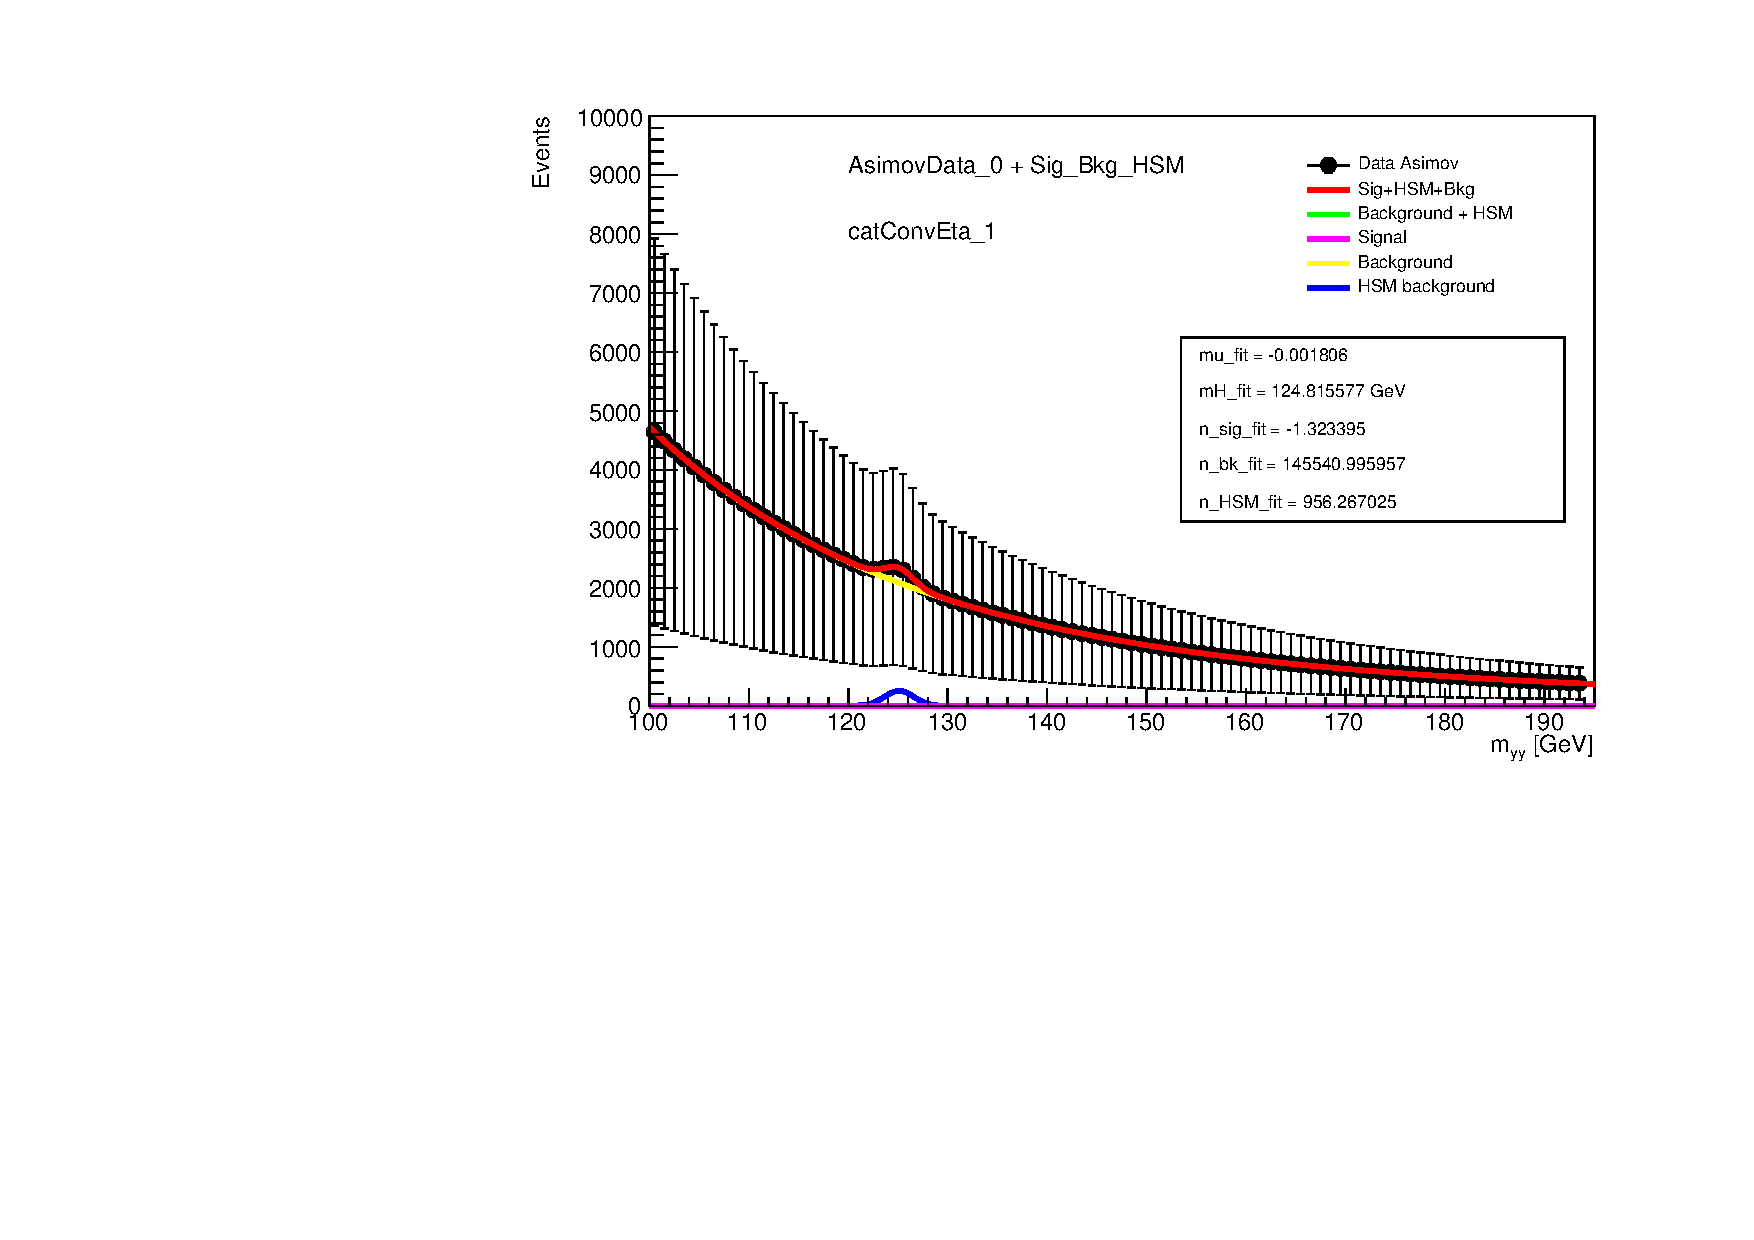
\includegraphics[width=1.\textwidth]{Pres_Images/HGam/HSM_AsimovData_0_catConvEta_1.pdf}
		\vfill
	\end{frame}

	\begin{frame}{Asimov $\mu$=1, m$_H$=125 GeV}
		\vfill
		\centering
		\includegraphics[width=1.\textwidth]{Pres_Images/HGam/HSM_AsimovData_1_125_catConvEta_1.pdf}
		\vfill
	\end{frame}
	
	\begin{frame}{Fiducial: 125 GeV}
		\vfill
		\centering
		\begin{table}[tbp]
			\centering
			\resizebox{11cm}{!}{
				\begin{tabular}{lcccccccc}
					\toprule[1.5pt]
					Cat [125 GeV]	&  n\_all	& n\_cut13	& n\_fidHigh	& cut/fidHigh	& fidHigh/all	& n\_fidLow	& cut/fidLow	& fidLow/all \\
					\midrule
					no & 16807.8 & 5470.83 & 6622.02 & 0.826157 & 0.433171 & 7341.79 & 0.745164 & 0.48034	\\
					1 & 16807.8 & 842.033 & 6622.02 & 0.127156 & 0.433171 & 7341.79 & 0.11469 & 0.48034		\\
					2 & 16807.8 & 1405.32 & 6622.02 & 0.212219 & 0.433171 & 7341.79 & 0.191414 & 0.48034	\\
					3 & 16807.8 & 408.892 & 6622.02 & 0.0617472 & 0.433171 & 7341.79 & 0.0556937 & 0.48034	\\
					4 & 16807.8 & 527.038 & 6622.02 & 0.0795886 & 0.433171 & 7341.79 & 0.071786 & 0.48034	\\
					5 & 16807.8 & 1598.8 & 6622.02 & 0.241436 & 0.433171 & 7341.79 & 0.217767 & 0.48034		\\
					6 & 16807.8 & 690.55 & 6622.02 & 0.104281 & 0.433171 & 7341.79 & 0.0940575 & 0.48034	\\
					
					\bottomrule[1.5pt]
				\end{tabular}
			}
			\caption{\centering Number of events and efficiencies for \texttt{cutFlow>13}, \texttt{isFiducialHighMyy} and \texttt{isFiducialLowMyy} cuts. $m_X=125$ GeV with \texttt{catConvEta} categorisation}
		\end{table}
		\vfill
	\end{frame}

	\begin{frame}{Production mods inc}
		\vfill
		\centering
		\begin{table}[tbp]
			\centering
			\resizebox{11cm}{!}{
				\begin{tabular}{lcccccccc}
					\toprule[1.5pt]
					Cat
					& \multicolumn{2}{c}{110 GeV}	
					& \multicolumn{2}{c}{125 GeV}
					& \multicolumn{2}{c}{130 GeV}	
					& \multicolumn{2}{c}{140 GeV} \\
					
					\midrule
					
					& \textbf{All} & \textbf{Fid\_High}
					& \textbf{All} & \textbf{Fid\_High}
					& \textbf{All} & \textbf{Fid\_High}
					& \textbf{All} & \textbf{Fid\_High} \\
					
					\cmidrule(lr){2-3} \cmidrule(lr){4-5} \cmidrule(lr){6-7} \cmidrule(lr){8-9}
					no & 0.163719 & 0.0106515 & 0.158653 & 0.0275281 & 0.157113 & 0.03305   & 0.154228 & 0.0439428 	\\
					1  & 0.329207 & 0.260816  & 0.28836  & 0.217073  & 0.275966 & 0.202788  & 0.252775 & 0.174647 	\\
					2  & 0.168929 & 0.0348676 & 0.172123 & 0.0522419 & 0.173095 & 0.0579295 & 0.174916 & 0.069153	\\
					3  & 0.134046 & 0.175762  & 0.127847 & 0.176196  & 0.125924 & 0.17634   & 0.122273 & 0.176629	\\
					4  & 0.343184 & 0.274333  & 0.309866 & 0.237343  & 0.299803 & 0.225312  & 0.281032 & 0.201683	\\
					5  & 0.136881 & 0.0645004 & 0.12726  & 0.086883  & 0.124344 & 0.0941893 & 0.118891 & 0.108577	\\
					6  & 0.114249 & 0.158083  & 0.135306 & 0.183131  & 0.14171  & 0.19133s  & 0.153712 & 0.207507	\\
					\bottomrule[1.5pt]
				\end{tabular}
			}
			\caption{\centering abs(eff$_{prod}$ - eff$_{ggH}$)/ eff$_{ggH}$ vs abs(cx$_{prod}$ - cx$_{ggH}$)/ cx$_{ggH}$ other production modes systematic uncertainties}
		\end{table}
		\vfill
	\end{frame}
		
	
\end{document}